\documentclass[12pt]{article}
\usepackage{graphicx} % For including graphics
\usepackage{hyperref} % For URLs and hyperlinks
\usepackage{amsmath} % For math symbols
\usepackage{enumitem} % For customized lists
\usepackage{geometry} % For page margins
\usepackage{xcolor} % For colored text
\usepackage{titlesec} % For title formatting
\usepackage{fancyhdr} % For headers
\usepackage{setspace} % For spacing
\usepackage{graphicx}
\usepackage{gensymb} % For addding degree symbol
\usepackage{multirow}
\usepackage{adjustbox} % For scaling the table
\usepackage{array} % For defining column widths and centering
\usepackage{geometry} % For margin adjustments
\usepackage{booktabs} % For better looking tables
\usepackage{caption}
\usepackage{subcaption}
\usepackage{float}
\usepackage{rotating}      % For sideways tables
\usepackage{tabularx}      % For automatically adjusting column widths
\usepackage{enumitem}      % For controlling list spacing
\usepackage{placeins}  % For \FloatBarrier
\usepackage{caption}

% Page setup
\geometry{a4paper, margin=0.75in} % Adjust margins to allow more space
\setlength{\parindent}{0pt} % Remove indentation
\captionsetup{font=scriptsize}  % Change 'small' to any size: footnotesize, scriptsize, etc.

\setlength{\parskip}{1em} % Adjust spacing between paragraphs



\renewcommand{\arraystretch}{1.2} % Adjusts the row height

% Title formatting with indentation for sections
% \titleformat{\section}{\bfseries\large\hspace*{1cm}}{\thesection.}{1em}{}
% \titleformat{\subsection}{\bfseries\hspace*{1cm}}{\thesubsection.}{1em}{}
% \titleformat{\subsubsection}{\bfseries\hspace*{2cm}}{\thesubsubsection.}{1em}{}

% Adjust paragraph indentation
\newenvironment{indentedsection}{
    \setlength{\parindent}{1cm} % Indent paragraphs
    \setlength{\leftskip}{1cm} % Indent entire section content
}{}

% Header setup
\pagestyle{fancy}
\fancyhf{}
\fancyhead[L]{Group No: C1}
\fancyhead[C]{ME 407 -- Fall 2024}
\fancyhead[R]{\thepage}

% Horizontal line
\renewcommand{\headrulewidth}{0.4pt}


% Begin Document
\begin{document}

% Main title and keyword section
\begin{center}
    \vspace{1em} % Add some space
    \textbf{\LARGE CONCEPTUAL DESIGN}\\
    \vspace{1em} % Add some space
\end{center}

% Start of sections
\section{Introduction}

This report presents and details the conceptual design part for the project of a Table Tennis Ball Pitcher Machine. By guide of the functional decomposition chart, project requirements and design criteria, and using the function alternatives developed in the morphological chart, different concepts are generated. These concepts are then evaluated in order by the evaluation criteria, and the best concept is chosen to meet the requirements and carry out all functions in the most efficient and effective way.

\section{Concept Development and Presentation}

Concept development and presentation are about turning ideas into clear plans and sharing them effectively. Concept development involves brainstorming, researching, and improving ideas to make them practical. Presentation is about explaining these ideas clearly using stories, visuals, and persuasive communication. Together, they help bring creative ideas to life and make them useful and understandable.

The list form and chart form of the functional decomposition we created during the concept development phase are given below (Fig. \ref{fig:fd}).

\begin{itemize}
    \item Launching the Balls to Desired Places
    \begin{itemize}
        \item Throwing the balls with a desired spin:
        \begin{itemize}
            \item Giving spin to the ball
            \item Controlling the spin
        \end{itemize}
        \item Throwing the balls with a desired speed:
        \begin{itemize}
            \item Giving speed to the ball
            \item Controlling the speed
        \end{itemize}
        \item Throwing the balls with a desired yaw angle:
        \begin{itemize}
            \item Giving yaw angle to the launching mechanism
            \item Controlling the yaw angle
        \end{itemize}
        \item Throwing the balls with a desired pitch angle:
        \begin{itemize}
            \item Giving pitch angle to the launching mechanism
            \item Controlling the pitch angle
        \end{itemize}
    \end{itemize}

    \item Accepting User Inputs
    \begin{itemize}
        \item Accepting frequency information from the user
        \item Accepting trajectory information from the user
        \item Accepting numerical information from the user
        \item Allowing user to position the device
    \end{itemize}

    \item Managing the Supply of the Balls
    \begin{itemize}
        \item Preventing balls from escaping
        \item Storing the balls
        \item Feeding the balls from storage:
        \begin{itemize}
            \item Transferring the balls from storage
            \item Controlling the ball feed from storage
        \end{itemize}
        \item Feeding to launching:
        \begin{itemize}
            \item Transferring the balls to launch
            \item Controlling the ball feed for launching
        \end{itemize}
        \item Managing the frequency of the ball supply:
        \begin{itemize}
            \item Giving the balls the desired frequency
            \item Controlling the ball frequency
        \end{itemize}
    \end{itemize}
\end{itemize}

\begin{figure}[H]
    \centering
    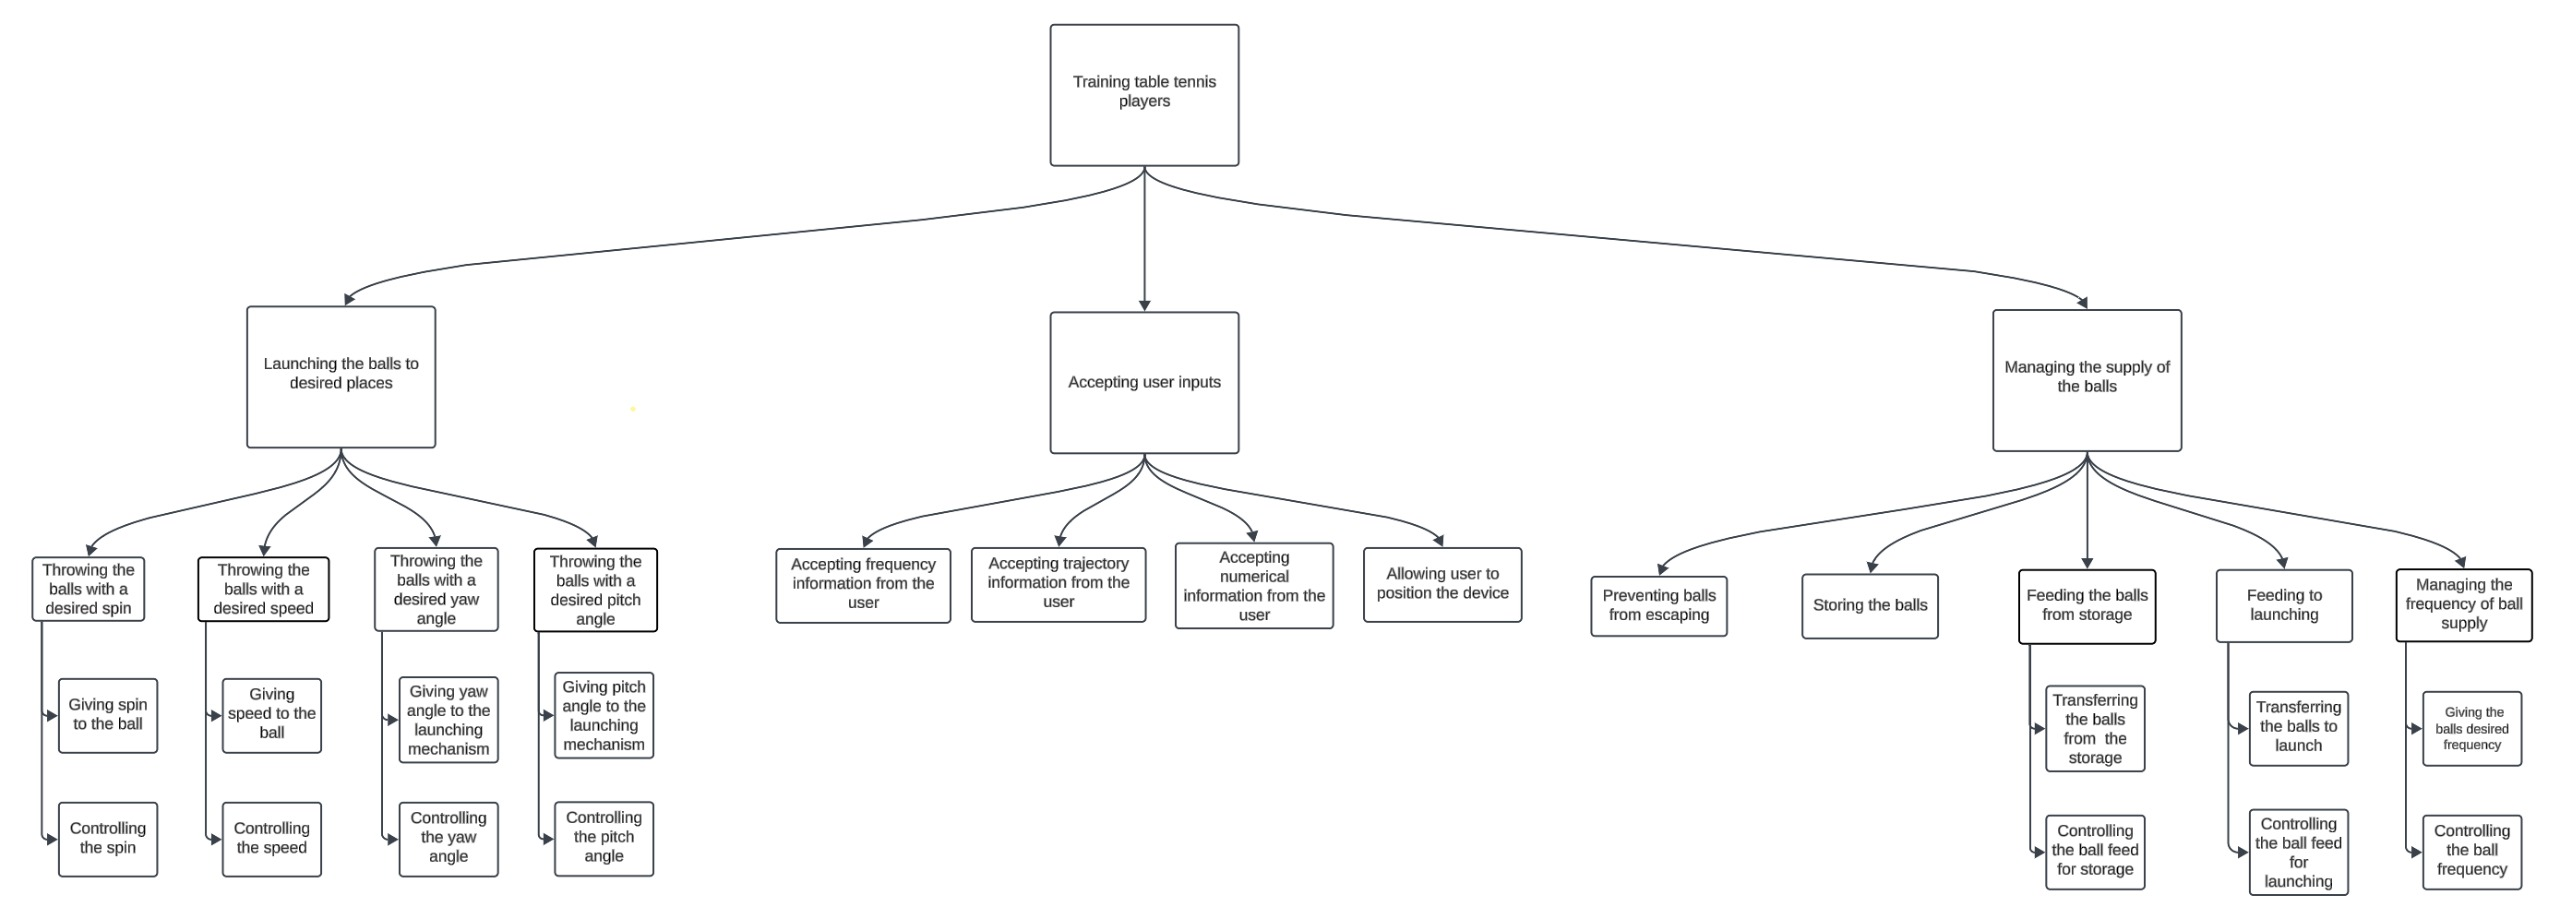
\includegraphics[width=0.9\linewidth]{fd.jpeg}
    \caption{Functional Decomposition}
    \label{fig:fd}
\end{figure}

The morphological chart containing the solutions of the functions included in functional decomposition is located in the Appendix \ref{app:morpho}.

The detailed explanation of each concepts are given below:

    
    \textbf{Concept 1:}
    
    The balls are to be stored by using a groove mechanism (as shown in Figure ~\ref{fig:groove_mechanism}) while providing recyclability of the balls with a net (Figure ~\ref{fig:net} ). Then the balls are transferred from the storage by a vertical spiral mechanism (Figure ~\ref{fig:spiral}) dictated with a stepper motor. A rotating pusher (Figure ~\ref{fig:rotating_pusher}) at the end of the vertical spiral mechanism is used to direct the balls coming from the spiral to the launching mechanism with desired frequency. The 3 wheel mechanism (Figure ~\ref{fig:3wheel}), which is controlled by DC motors is benefitted to give and control the spin options and speed of the balls. The yaw angle value is controlled by using gears (Figure ~\ref{fig:gear1}), which rotates the head. The pitch angle is controlled by a four bar mechanism (Figure ~\ref{fig:fourbar}). Both controlling mechanisms are connected with servo motors to rotate the head in the desired directions. The trajectory and frequency information are accepted from the user with an integrated controller (Figure ~\ref{fig:integrated}). Accepting numerical information from the user is provided by using a potentiometer with buttons (Figure ~\ref{fig:pot}). Finally, the user is allowed to fix the device to the table by using clamps (Figure ~\ref{fig:clamp}).

    \textbf{Concept 2:}
    
    The balls are to be stored by using a box (Figure ~\ref{fig:box}), while providing recyclability of the balls with a net (Figure ~\ref{fig:net}). Then the balls are transferred from the storage to the launcher by a translating box (Figure ~\ref{fig:translating_box}) with a stepper motor. The balls are transferred to launch by the effect of gravity (represented at Figure ~\ref{fig:gravity}), while the desired frequency is provided by a rotating hole (Figure ~\ref{fig:rotating_hole}). The orientation of the hole determines the frequency. The 4 wheel mechanism (Figure ~\ref{fig:4wheel}), which is controlled by BLDC motors is benefitted to give and control the spin options and speed of the balls. The yaw angle values are controlled by using four bar mechanisms (Figure ~\ref{fig:fourbar_yaw}), and pitch angle values are controlled by a rope controlled head pulley (Figure ~\ref{fig:rope})  to rotate the head in the desired directions. Both mechanisms are dictated by servomotors. The trajectory and frequency information are accepted from the user with an integrated controller (Figure ~\ref{fig:integrated}). Accepting numerical information from the user is provided by using a potentiometer with buttons (~\ref{fig:pot}). Finally, the user is allowed to fix the device to the table by using clamps (Figure ~\ref{fig:clamp}).

    \textbf{Concept 3:}

    The balls are to be stored by using a box (Figure ~\ref{fig:box}) while providing recyclability of the balls with a net (Figure ~\ref{fig:net}). Then the balls are transferred from the storage to the launcher by a vertical spiral mechanism (shown at Figure ~\ref{fig:spiral}) dictated with a stepper motor. A rotating pusher (Figure ~\ref{fig:rotating_pusher}) at the end of the vertical spiral mechanism is used to direct the balls coming from the spiral to the launching mechanism and give the desired launch frequency. The 2 wheel mechanism (Figure ~\ref{fig:2wheel}), which is controlled by DC motors is benefitted to give and control the spin options and speed of the balls. The control of yaw and pitch angle is provided by bevel gear mechanisms (Figures ~\ref{fig:bevel} and ~\ref{fig:bevel_yaw}). Both controlling mechanisms are connected with servo motors to rotate the head in the desired directions. The trajectory and frequency information are accepted from the user with a wired remote (Figure ~\ref{fig:wired}). Accepting numerical information from the user is provided by using a potentiometer with buttons (Figure ~\ref{fig:pot}). Finally, the user is allowed to fix the device to the table by using a clamp mechanism (Figure ~\ref{fig:clamp}).

    \textbf{Concept 4:}

    The balls are to be stored by using a groove mechanism (Figure ~\ref{fig:groove_mechanism}) while providing recyclability of the balls with a net (Figure ~\ref{fig:net}). Then the balls are transferred from the storage to the launcher by a maltese wheel mechanism (Figure ~\ref{fig:maltese}) dictated with a stepper motor. Also, this maltese wheel is used to direct the balls to the launching mechanism by the pushing effect of the consecutive balls and helps give the desired frequency. The 3 wheel mechanism (Figure ~\ref{fig:3wheel}), which is controlled by BLDC motors is benefitted to give and control the spin options and speed of the balls. The control of yaw and pitch angle values are done by gear mechanisms (Figures ~\ref{fig:gear} and ~\ref{fig:gear2}), which are connected with servo motors. The gears control the pitch and yaw angle values by rotating the head and base, respectively. The trajectory and frequency information are accepted from the user with an integrated controller (Figure ~\ref{fig:integrated}). Accepting numerical information from the user is provided by using a potentiometer with buttons (Figure ~\ref{fig:pot}). Finally, the user is allowed to fix the device to the table by using clamps (Figure ~\ref{fig:clamp}).

    \textbf{Concept 5:}

    The balls are to be stored by using a tunnel mechanism (Figure ~\ref{fig:tunnel_mechanism}) while providing recyclability of the balls with a net (Figure ~\ref{fig:net}). This tunnel is placed between a maltese wheel (Figure ~\ref{fig:maltese}) on bottom and a slider crank (Figure ~\ref{fig:slider_crank}) at top, the maltese wheel enables the ball entrance to the tunnel from the net, whereas the slider crank transfers balls to the launching with desired frequency. These maltese wheels are activated with stepper motors. The 2 tension belt with spinning head mechanism (Figure ~\ref{fig:2tension}), which is controlled by BLDC motors is benefitted to give and control the spin options and speed of the balls. The control of pitch angle is provided by a worm gear mechanism (Figure ~\ref{fig:worm}) and the yaw angle is controlled by a gear mechanism (Figure ~\ref{fig:gear2}), rotating the head from the base. Both controlling mechanisms are connected with servo motors to rotate the head in the desired directions. The trajectory and frequency information are accepted from the user with an integrated controller (Figure ~\ref{fig:integrated}). Accepting numerical information from the user is provided by using an encoder (Figure ~\ref{fig:encoder}) . Finally, the user is allowed to fix the device to the table by using clamps (Figure ~\ref{fig:clamp}).

    \textbf{Concept 6:}

    The balls are to be stored by using a groove mechanism (Figure ~\ref{fig:groove_mechanism}) while providing recyclability of the balls with a net (Figure ~\ref{fig:net}). A maltese wheel (Figure ~\ref{fig:maltese}) is benefitted to raise the balls to a selected elevation and the transferring process from the storage is initiated. Then the balls are transferred to the launcher by the effect of gravity (represented at Figure ~\ref{fig:gravity}) . The desired frequency is given by the movement of a lid mechanism (Figure ~\ref{fig:lid_mechanism}). The 3 wheel mechanism (Figure ~\ref{fig:3wheel}) , which is controlled by DC motors is benefitted to give and control the spin options and speed of the balls. The control of yaw and the pitch angle is controlled by four bar mechanisms (Figures ~\ref{fig:fourbar_yaw} and ~\ref{fig:fourbar}). Both controlling mechanisms are connected with servo motors to rotate the head in the desired directions. The trajectory and frequency information are accepted from the user with an integrated controller (Figure ~\ref{fig:integrated}). Accepting numerical information from the user is provided by using a potentiometer with buttons (Figure ~\ref{fig:pot}). Finally, the user is allowed to fix the device to the table by using clamps (Figure ~\ref{fig:clamp}).

    \textbf{Concept 7:}

    The balls are to be stored by using a groove mechanism (Figure ~\ref{fig:groove_mechanism}) while providing recyclability of the balls with a net (Figure ~\ref{fig:net}). Then the balls are transferred from the storage to the launcher by a belt mechanism (Figure ~\ref{fig:belt}) dictated with a stepper motor. A maltese wheel (Figure ~\ref{fig:maltese_wheel} ) mechanism is used to direct the balls coming from the vertical belt to the launching mechanism, also the desired frequency is given. The 2 wheel mechanism (Figure ~\ref{fig:2wheel}), which is controlled by BLDC motors is benefitted to give and control the spin options and speed of the balls. The pitch angle value is controlled by using bevel gear (Figure ~\ref{fig:bevel}), and yaw angle value is controlled by a worm gear (Figure ~\ref{fig:worm_yaw}). Both controlling mechanisms are connected with servo motors to rotate the head in the desired directions. The trajectory and frequency information are accepted from the user with an integrated controller (Figure ~\ref{fig:integrated}). Accepting numerical information from the user is provided by using a potentiometer with buttons (Figure ~\ref{fig:pot}). Finally, the user is allowed to fix the device to the table by using clamps (Figure ~\ref{fig:clamp} ).



    \textbf{Concept 8:}

    The balls are to be stored by using a groove mechanism (Figure ~\ref{fig:groove_mechanism}) while providing recyclability of the balls with a net (Figure ~\ref{fig:net}). Then the balls are transferred from the storage to a vertical tube by a maltese wheel (Figure ~\ref{fig:maltese}) dictated with a stepper motor. The end of the tube is at a higher elevation from the launch. The balls are released from the tip to the launching mechanism. The gravitational force (represented at Figure ~\ref{fig:gravity}) provides the transfer to launch. The required frequency is set by a hinge mechanism (Figure ~\ref{fig:hinge_mechanism}), the movement of the hinge mechanism determines the frequency. The 4 wheel mechanism (Figure ~\ref{fig:4wheel}), which is controlled by BLDC motors is benefited to give and control the spin options and speed of the balls. The pitch angle value is controlled by using a four bar mechanism (Figure ~\ref{fig:fourbar}), and yaw angle value is controlled by a gear, which rotates the head (Figure ~\ref{fig:gear2}) . Both controlling mechanisms are connected with servo motors to rotate the head in the desired directions. The trajectory and frequency information are accepted from the user with an integrated controller (Figure ~\ref{fig:integrated}). Accepting numerical information from the user is provided by using an encoder (Figure ~\ref{fig:encoder}). Finally, the user is allowed to fix the device to the table by using clamps (Figure ~\ref{fig:clamp}).



    \subsection{Calculations}


    \textbf{Launcher wheels required angular speed:}

    Maximum required speed of the ball is 30 m/s, so maximum contact speed should also be $30 m/s$. Assuming there is no slip between ball and launcher wheel, and no spin is given:

    \begin{align}
        V &= \omega \cdot r \implies 30 \, \text{m/s} = \omega \cdot 0.03 \, \text{m} \\
        \omega &= 1000 \, \text{rad/s} = 9550 \, \text{rpm}
    \end{align}
    
    Where $\omega$ is angular speed and V is linear speed of the outer surface of the ball. In this case, slip is assumed as $\%20$.
    
    \begin{align}
        \omega' &= \omega \cdot 1.2 = 11460 \, \text{rpm}
    \end{align}

    Speed requirements considering spin: 
    
    \begin{minipage}{0.48\textwidth}
        \centering
        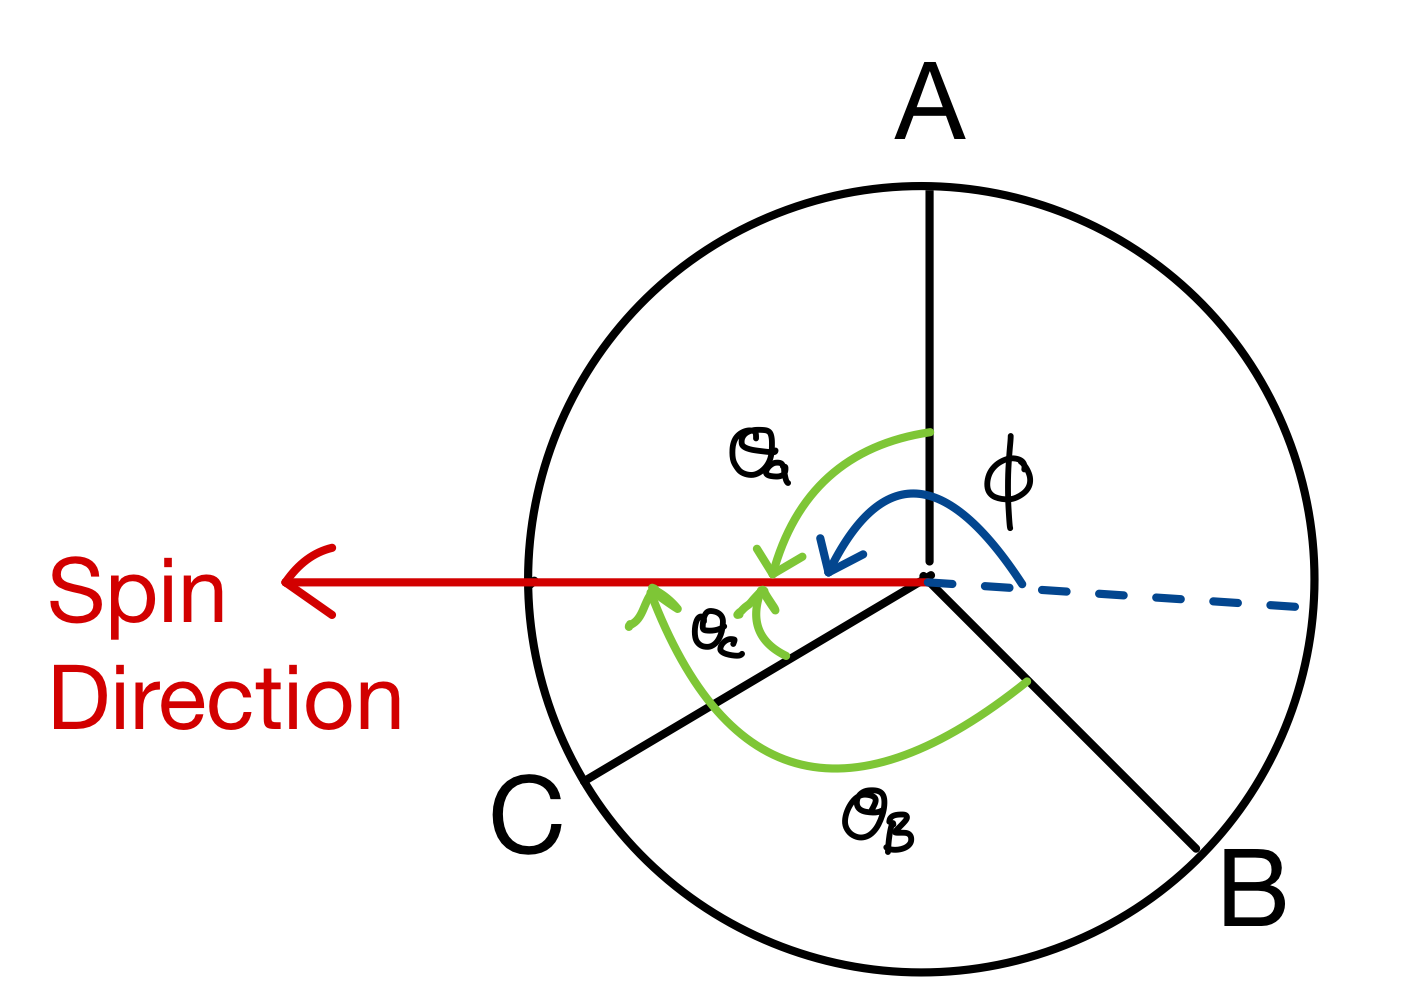
\includegraphics[width=60mm]{calculation_graph.png}
        \captionof{figure}{Free body diagram of the ball}
        \label{fig:wholesales}
    \end{minipage}
    \begin{minipage}{0.48\textwidth}
    Speed direction is into the page 
    \begin{align}
        V_a &= V + \omega \cdot r \cdot \sin(\theta_a) \\
        V_b &= V - \omega \cdot r \cdot \sin(\theta_b) \\
        V_c &= V - \omega \cdot r \cdot \sin(\theta_c)
    \end{align}
    
    where,
    \begin{align}
        \theta_a &= \phi - 90^\circ \\
        \theta_b &= 330^\circ - \phi \\
        \theta_c &= 210^\circ - \phi
    \end{align}
    
    \end{minipage}

    \textbf{Torque requirement of the launcher wheels:}

    This torque requirement is determined by impulse calculations. Ball mass is $m=2.7$ grams.

    \begin{align}
        J &= F \cdot t = \Delta p = m \cdot V \\
        &= 2.7 \cdot 10^{-3} \, \text{kg} \cdot 30 \, \text{m/s} \\
        &= 0.075 \, \text{N·s}
    \end{align}
    
    Where $F$ is impulse, $t$ is contact time, and $F$ is required force to be applied.

    If the contact time is assumed as $0.1$ seconds, the required torque of motors should be,

    \begin{align}
        \frac{J}{3t} \cdot r &= \frac{0.075}{3 \cdot 0.1} \cdot 0.030 \\
                              &= 0.0075 \, \text{N·m}
    \end{align}
    
    
    \textbf{Required torque for giving the pitch angle:}

    The total mass of the head mechanism will be around 250 gram and center of the mass will be approximately 15 cm away from the joint. Hence the required torque to be applied from the joint could be calculated by,

    \begin{align}
        T &= F \cdot d = M \cdot g \cdot d \\
          &= 0.25 \cdot 9.81 \cdot 0.15 \\
          &= 0.368 \, \text{N·m}
    \end{align}
    
    where d is distance of mass center from the joint; M is total mass of the head.
    

\section{Evaluation of Concepts}

The evaluation of criteria was conducted using the Analytic Hierarchy Process (AHP) method. Initially, Saaty's Fundamental scale for pairwise comparison is utilized. This method employs a pairwise comparison approach, which means that each criterion is compared to every other criterion on Saaty's 1-9 scale of relative importance. This scale goes from 1 (equal importance) to 9 (absolute importance), with intermediate values (2, 4, 6, 8) denoting nuanced assessments. Then these values were normalized, and weighted averages were calculated to ensure a consistent and unbiased evaluation framework.

In addition to assessing each concept, the evaluation criteria were also applied to analyze the functions and corresponding solutions presented in the morphological chart. For each function, a decision matrix was constructed, and the solution with the highest score in each matrix was identified as the optimal choice for that specific function. This systematic approach ensured that both the overall concepts and individual functions were evaluated objectively.


Our design criteria are as follows:


\begin{enumerate}
    \item \textbf{Serving Frequency:} Can throw 80 balls per minute and more. Also, adjustable within 25-80 balls per minute.
    \item \textbf{Feeding the Ball}: Allows for uninterrupted training with desired frequency.
    \item \textbf{Serving Speed:} Adjustable between 4 m/s and 25 m/s. Can throw balls at 25 m/s and more.
    \item \textbf{Preventing Balls from Escaping:} The design can collect balls that came up to 1 meter height on its side.
    \item \textbf{Selectable Serving Modes:} Supports various training modes.
    \item \textbf{Giving Yaw and Pitch Angle:} Angles need to be adjustable within specified ranges accurately.
    \item \textbf{Portability:} Less than the maximum weight which is 15 kg, easy to set up.
    \item \textbf{Capacity:} Minimum storage of 100 balls.
    \item \textbf{Ball Durability:} Balls should withstand at least 1000 throws.
    \item \textbf{Power Consumption:} Energy efficiency is prioritized.
    \item \textbf{Spin Options:} Ability to generate 36 spins for varied training.
    \item \textbf{User Interface:} It should be easy to use and should not contain complicated buttons.
    \item \textbf{Cost:} The design should be cost efficient, the cost of manufacturing must be less than 300 dolars.
    \item \textbf{No Spin (Bonus):} Throwing should be possible without spin.
    \item \textbf{Different Scenarios (Bonus):} Allow different types of throws, for example starting with a serve.
\end{enumerate}


Based on the design criteria, the evaluation criteria are derived as follows:
\begin{enumerate}
    \item \textbf{Maximum Attainable Serving Frequency:} The highest number of balls the machine can serve per second. Measures the machine's overall capability to serve balls at its highest possible rate, regardless of how the balls are fed. This criterion is derived from the "Serving Frequency" design criterion, as achieving a high maximum frequency ensures the machine can meet a wide range of performance requirements with flexibility for lower frequencies.

    \item \textbf{Serving Frequency Adjustment Accuracy:} The precision of frequency adjustment, measured as deviation from the target frequency. This criterion is also derived from "Serving Frequency," focusing on how accurately the machine can meet specific serving rates, crucial for scenarios that require controlled and consistent ball delivery.

    \item \textbf{Maximum Feeding Speed:} The rate at which the machine loads and serves balls from the reservoir, ensuring continuous and efficient operation without interruptions. Focuses specifically on the efficiency of the feeding mechanism to supply balls into the serving system at a consistent rate. This criterion is derived from the "Feeding the Balls" design criterion, as the ability to achieve a high feeding speed ensures the machine can handle demanding use cases while maintaining a smooth and consistent supply of balls to the serving mechanism.

    \item \textbf{Maximum Attainable Pitch and Yaw Angle:} The highest vertical and horizontal angle the machine can achieve, determining its capability to simulate lobs or high-arc serves and allowing it to target various positions across the table for diverse shot placement. This criterion is derived from the "Giving Yaw and Pitch Angle" design criterion, as evaluating the maximum angles ensures the machine can cover a wide range of shot trajectories and placements, providing versatility and precision in gameplay scenarios.


    \item \textbf{Ball Prevention Efficiency:} The proportion of prevented balls from escaping successfully and transferred to the reservoir. This criterion is derived from the "Preventing Balls from Escaping" design criterion, as it quantifies the effectiveness of the mechanism in retaining balls, ensuring minimal loss during operation and maintaining a consistent supply for serving.

    \item \textbf{Serving Accuracy:} Average deviation of the ball's landing point from the target. This criterion is derived from "Giving Yaw and Pitch Angle," "Serving Speed," and "Feeding the Balls" design criteria, as accurate targeting requires precise control over ball direction, velocity, and feeding consistency. Additionally, it depends on the "Serving Frequency" design criterion to ensure that accuracy is maintained even at the desired serving rates.  


    \item \textbf{Serving Precision:} Consistency of serving, measured as the standard deviation of ball landing points. This criterion is derived from "Giving Yaw and Pitch Angle," "Serving Speed," and "Feeding the Balls" design criteria, as consistent ball placement relies on stable directional control, speed regulation, and feeding. The "Serving Frequency" design criterion also plays a role by ensuring precision is upheld across various serving rates without performance degradation.


    \item \textbf{Maximum Attainable Serving Speed:} The fastest ball velocity the machine can achieve. This criterion is derived from "Feeding the Balls" and "Serving Speed" design criteria, as achieving high serving speeds requires efficient feeding of balls into the serving mechanism and robust control over the velocity imparted to the ball during the serving process.


    \item \textbf{Portability:} Subjective score based on factors such as weight, size, and transportability. This criterion is derived from the "Portability" design criterion, as it assesses how easy it is to move, transport, and store the machine, taking into account the overall design and physical characteristics that influence its mobility.

    \item \textbf{Reservoir Capacity:} Maximum number of balls the reservoir can hold. This criterion is derived from the "Capacity" design criterion, as it measures the machine's ability to store and supply a sufficient number of balls for uninterrupted operation, impacting both performance and convenience during extended use.

    \item \textbf{Ball Durability:} Percentage of wear or deformation observed on balls after a specified number of serves. This criterion is derived from the "Capacity" design criterion, as the ability to store and serve a large number of balls without causing excessive wear or damage directly impacts the longevity and performance of the balls over time.

    \item \textbf{Energy Consumption:} Average power usage during operation. This criterion is derived from the "Power Consumption" design criterion, as it measures the efficiency of the machine in terms of energy usage, reflecting how well the system optimizes power consumption during its operation.

    \item \textbf{Spin Options Variety:} Number of spin types the machine can generate (e.g., topspin, backspin, sidespin). This criterion is derived from the "Spin Options" design criterion, as it evaluates the variety of spin types the machine can produce, which directly affects the range of gameplay scenarios it can simulate.

    \item \textbf{Cost:} Total cost of manufacturing or purchasing the machine. This criterion is derived from the "Cost" design criterion, as it directly reflects the financial aspect of producing or acquiring the machine, factoring in materials, labor, and other associated expenses.

    \item \textbf{Ease of Manufacturing:} A subjective score reflecting the ease or difficulty of manufacturing the machine. This criterion is derived from all the design criteria, as the complexity of the overall design, including components like feeding mechanisms, serving accuracy, spin options, and portability, directly influences how easy or difficult it is to manufacture the machine.

    \item \textbf{Response Time:} The time the system takes to reach its target value after a command, indicating its speed and efficiency. This criterion is derived from "Serving Speed" and "Giving Yaw and Pitch Angle" design criteria, as the ability to quickly adjust the serving speed and angles directly affects how fast the machine can respond to commands and achieve the desired target values.


    \item \textbf{User Friendliness:} Focuses on the clarity of the controls, the simplicity of the process, and how quickly a user can achieve desired outcomes without confusion or excessive effort. This criterion is derived from the "User Interface" design criterion, as the design and layout of the interface directly influence how intuitive and straightforward the machine is for users to operate and achieve their desired settings.


    \item \textbf{Ease of Control:} Evaluates how straightforward and intuitive it is to manage, adjust, or optimize the system during development and operation, ensuring minimal complexity and effort. This criterion is derived from the overall functions of the machine, as it focuses on the designer's perspective, ensuring that the system’s functions are easily adjustable and controllable to achieve desired outcomes with precision and efficiency.

    \item \textbf{Ease of Mounting:} Measures how quickly and effortlessly the user can mount the device onto the setup. This criterion is derived from the "Portability" design criterion, as a portable design inherently involves considerations for simple and convenient mounting, ensuring that the device can be securely and efficiently attached or detached without requiring excessive effort or specialized tools.


    \item \textbf{Maximum Supplied Speed:} Evaluates the maximum speed that the system’s power source can provide to drive key functions such as serving frequency, feeding mechanisms, and serving speed. This criterion is derived from "Serving Frequency," "Feeding the Balls," and "Serving Speed" design criteria, as it focuses on the capability of the system’s core power source (most likely an electric motor but not restricted to one) to ensure optimal operation of these interconnected functions. It is critical for controlling and enabling the precise and efficient movement of these subsystems.

    
\end{enumerate}

The relative importance of the criteria is evaluated and presented in the matrix shown in Figure~\ref{fig:cvc1}. The normalized version of the evaluated criteria table, along with the derived weighting factors, is depicted in Figure~\ref{fig:cvc2}. These criteria and their corresponding weighting factors are important, as they will be used in selecting the best solution for each subfunction. In the following sections of the report, the weighting factors shown in Figure~\ref{fig:cvc2} will be considered.


\begin{figure}[H]
    \centering
    \rotatebox{90}{\includegraphics[width=\textheight]{cvc1.jpg}}
    \caption{Criteria vs Criteria Evaluation}
    \label{fig:cvc1}
\end{figure}

\begin{figure}[H]
    \centering
    \rotatebox{90}{\includegraphics[width=\textheight]{cvc2.jpg}}
    \caption{Criteria vs Criteria Evaluation Normalized}
    \label{fig:cvc2} 
\end{figure}

This section presents the decision matrices to evaluate the 20 subfunctions of the table tennis ball launcher design. Each subfunction was evaluated using several solution options, which were compared to a set of established evaluation criteria. The relative relevance of these criteria was determined by a pairwise comparison utilizing Saaty's Analytical Hierarchy Process (AHP), which generated weighting factors based on the criterion vs. criterion relative importance matrix.

The decision matrices use these weighting factors to identify the best solution for each subfunction. By carefully evaluating and rating each possibility against the criteria, decision matrices give a clear and rational foundation for selecting the best answer for each subfunction.




Five design alternatives were considered for giving spin to the ball. Based on a thorough decision matrix analysis, the three-wheel configuration was identified as the most suitable option as can be seen in Figure~\ref{fig:spin}. This design outperformed the two-wheel system with a rotating head and the four-wheel configuration in terms of efficiency and simplicity. The four-wheel setup posed challenges due to the complexity of synchronizing four independent motors, which could lead to slower response times. Meanwhile, the two-wheel system with a spinning head required additional time to adjust the head's motion to generate the desired spin. Thus, the three-wheel configuration was selected as the optimal solution for imparting spin to the ball.
\begin{figure}[H]
    \centering
    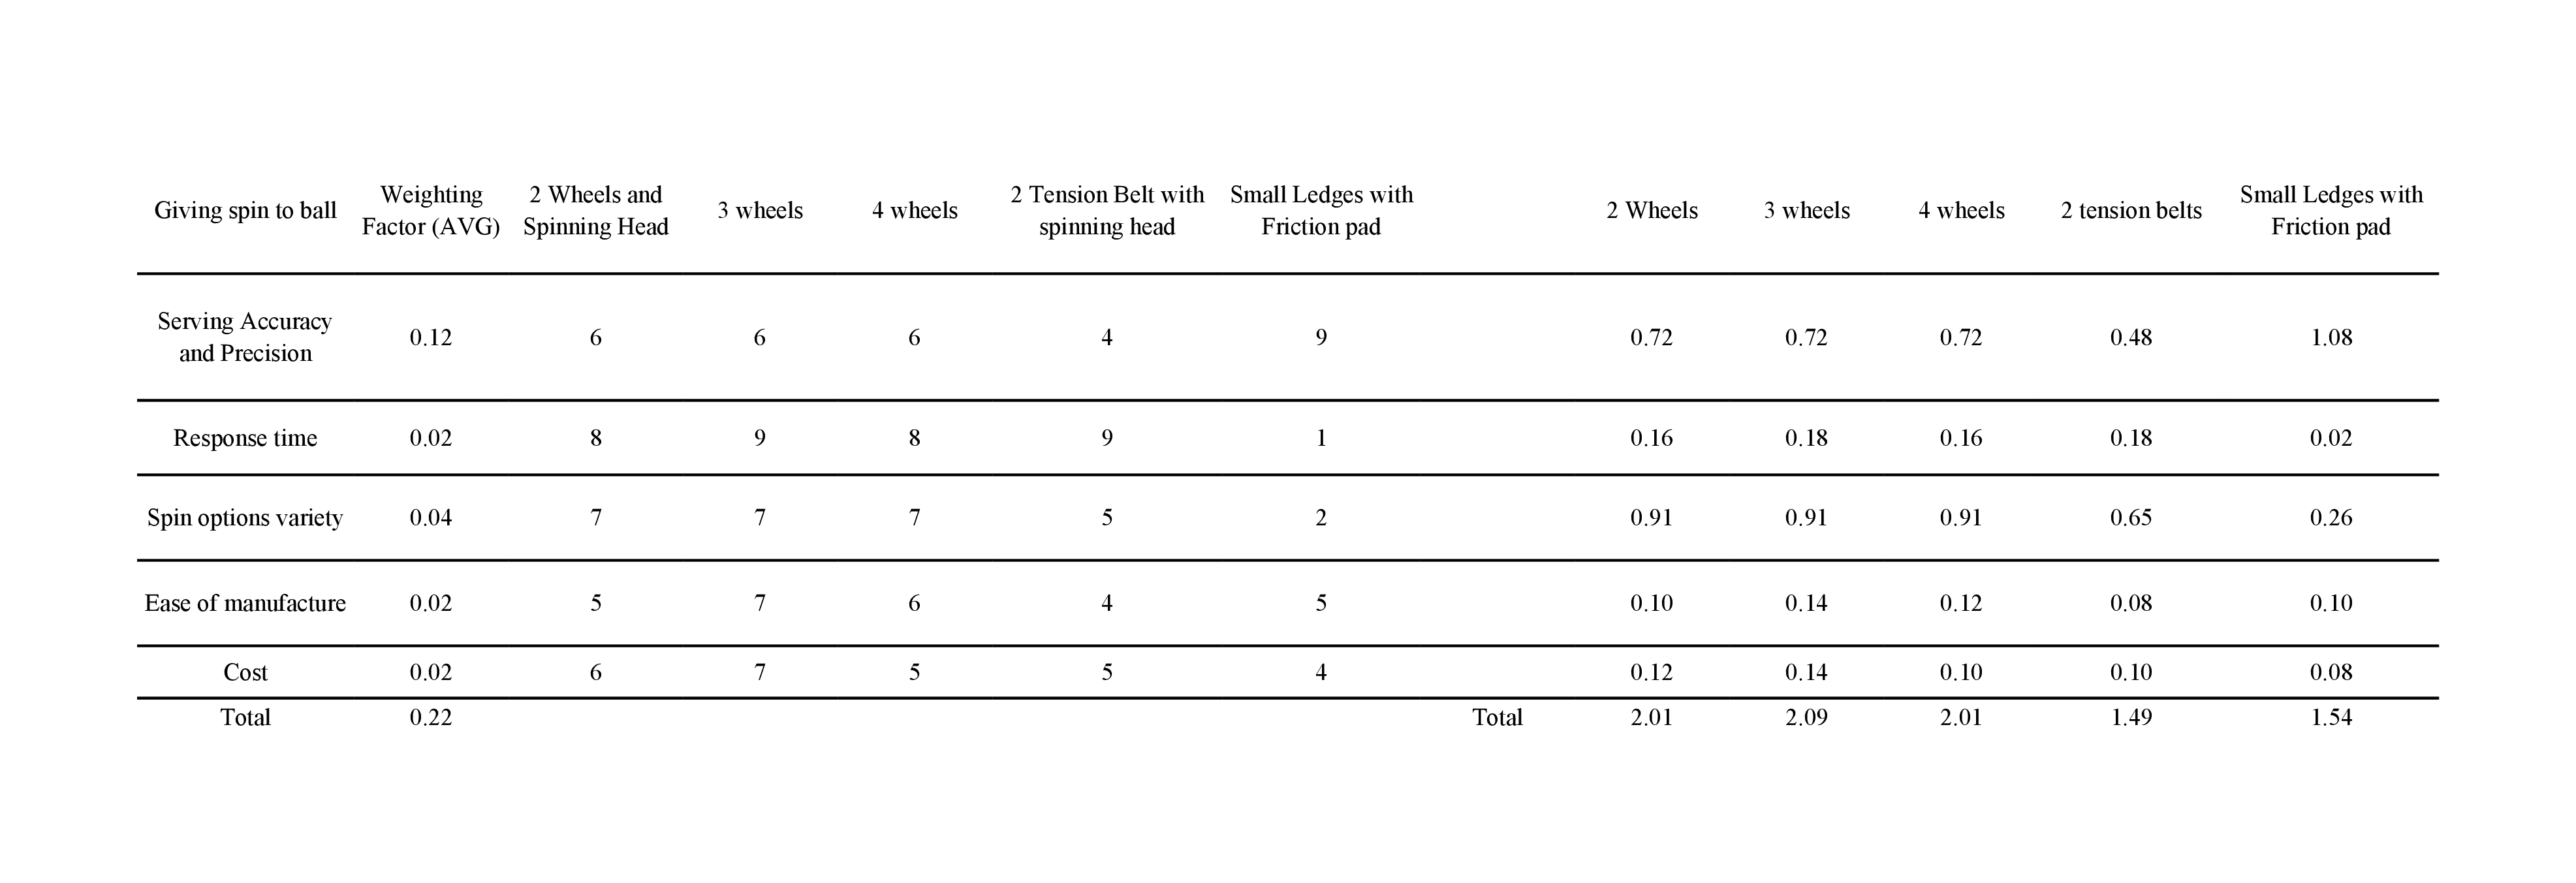
\includegraphics[width=1\textwidth]{Decision matrices/spin.png}
    \caption{Giving spin to the ball}
    \label{fig:spin}
\end{figure}



Three alternatives were considered for controlling spin: DC, BLDC, and stepper motors. Based on the decision matrix evaluation, BLDC motors were selected as the optimal solution. This choice was driven by their better accuracy and precision, as well as their ability to provide a higher maximum supplied speed compared to the other options.
\begin{figure}[H]
    \centering
    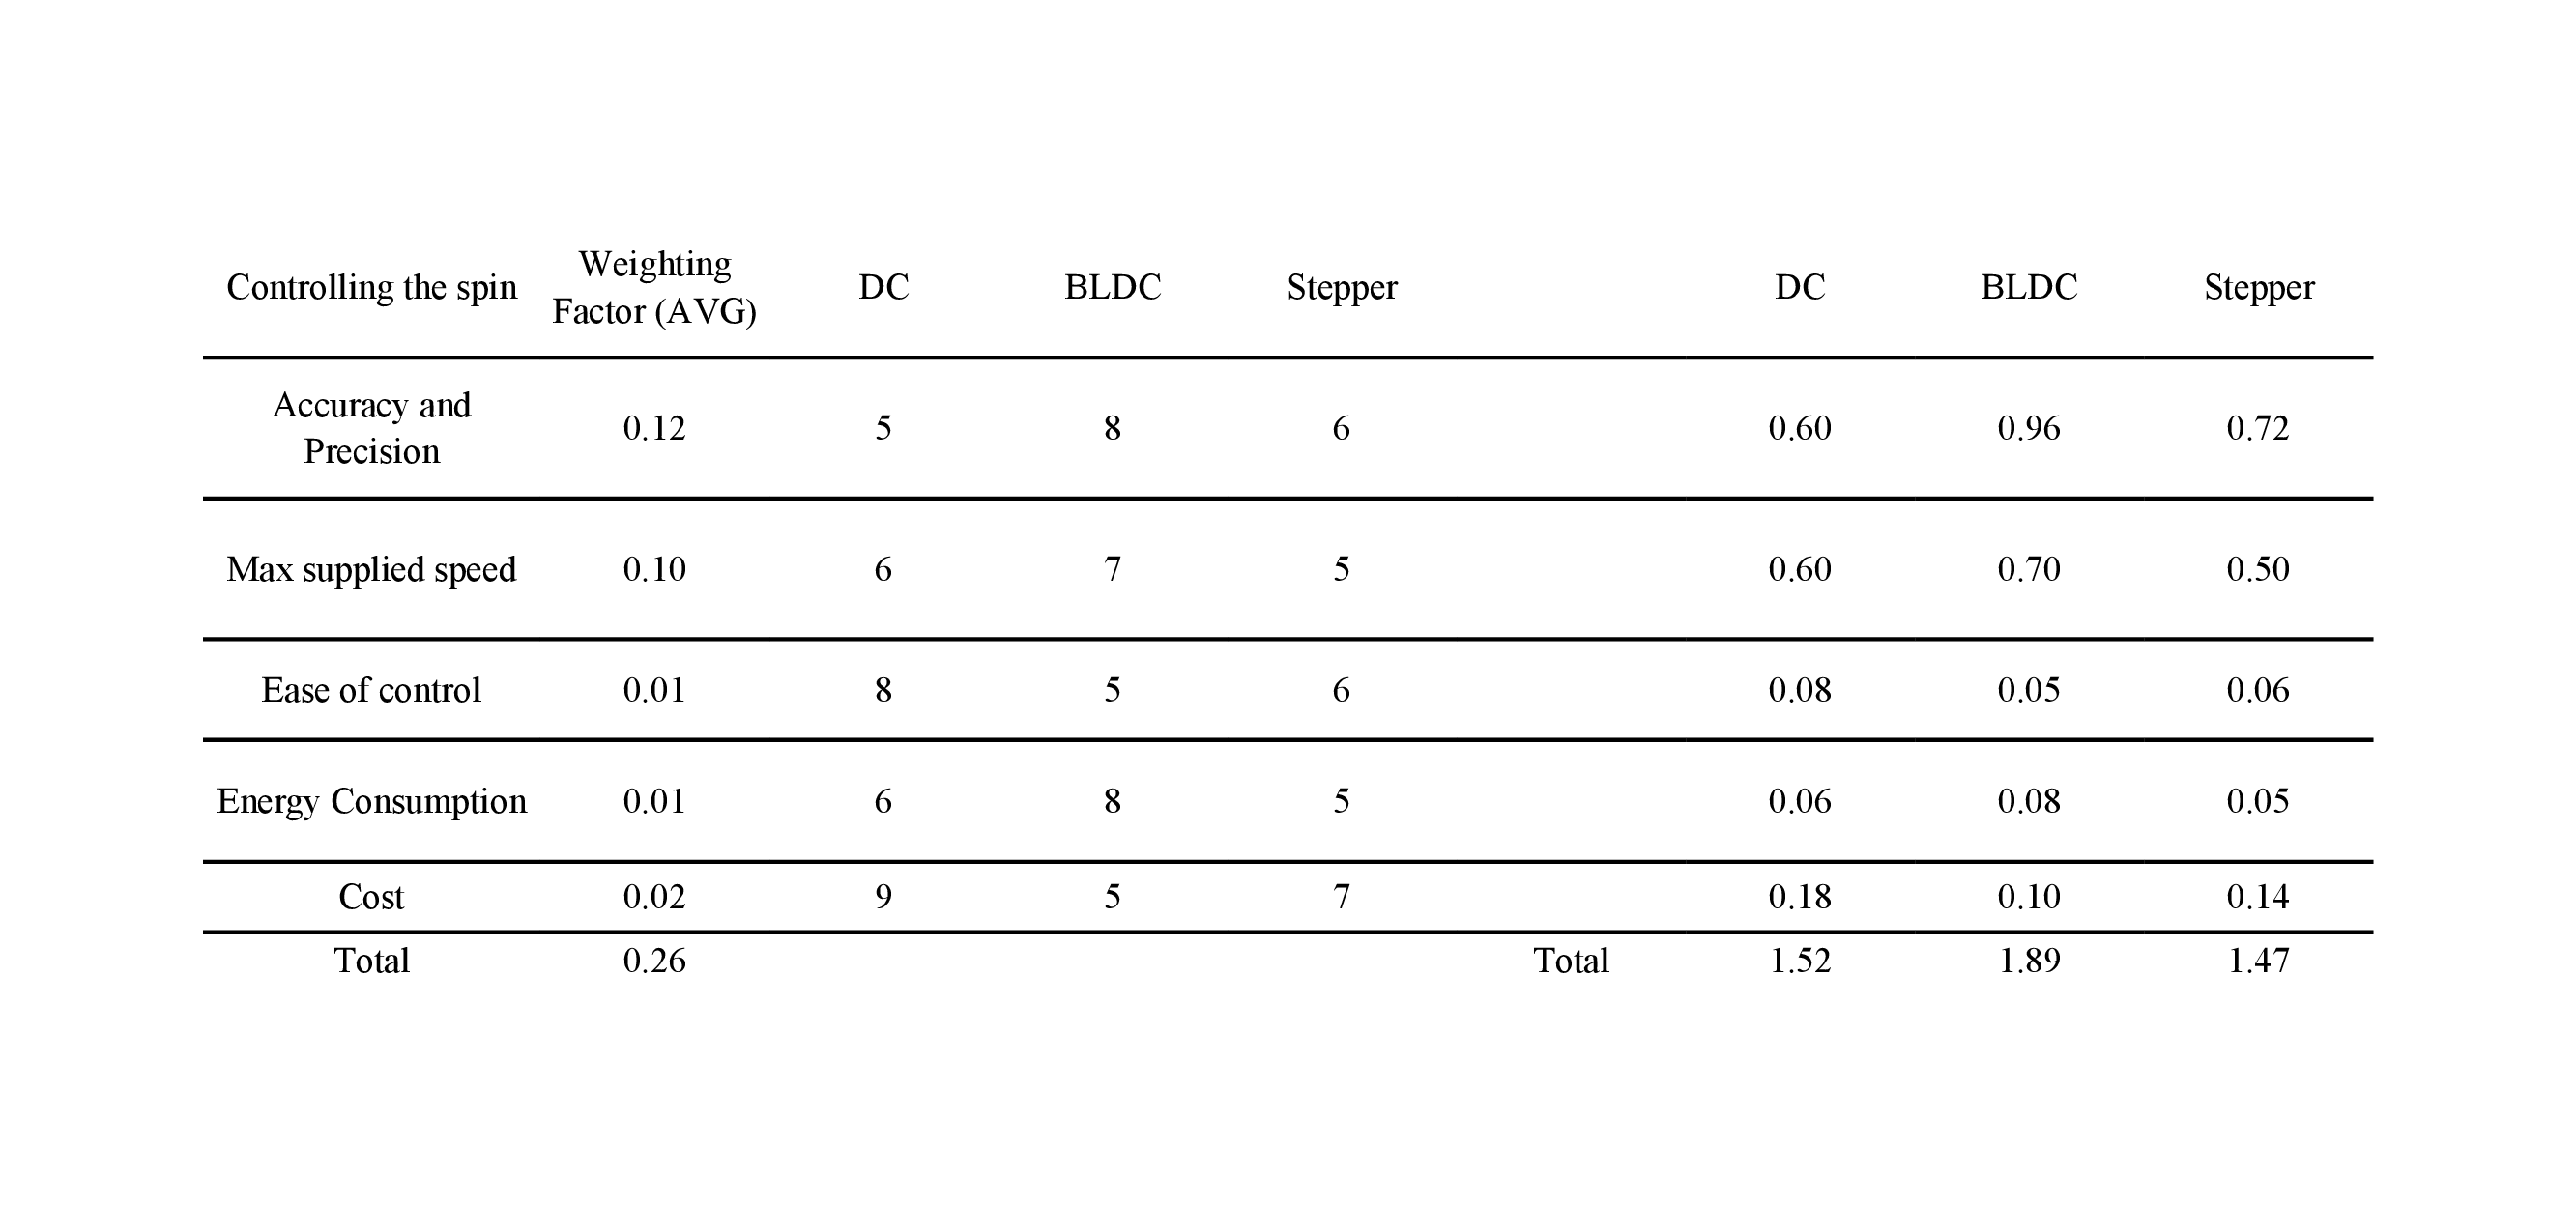
\includegraphics[width=0.8\textwidth]{Decision matrices/controlling spin.png}
    \caption{Controlling the spin}
\end{figure}


Six design alternatives were considered for giving speed to the ball. As with giving spin, the decision matrix evaluation identified the three-wheel configuration as the best alternative. It was also discussed in the context of achieving spin, the three-wheel design demonstrated significant advantages over the two-wheel system with a rotating head and the four-wheel configuration. The four-wheel setup posed challenges due to the complexity of synchronizing four independent motors, potentially increasing response time. Similarly, the two-wheel system with a spinning head required additional time to adjust the head's motion to generate the desired speed. Consequently, the three-wheel configuration was selected as the optimal solution for giving speed to the ball, consistent with its performance in spin application.

\begin{figure}[H]
    \centering
    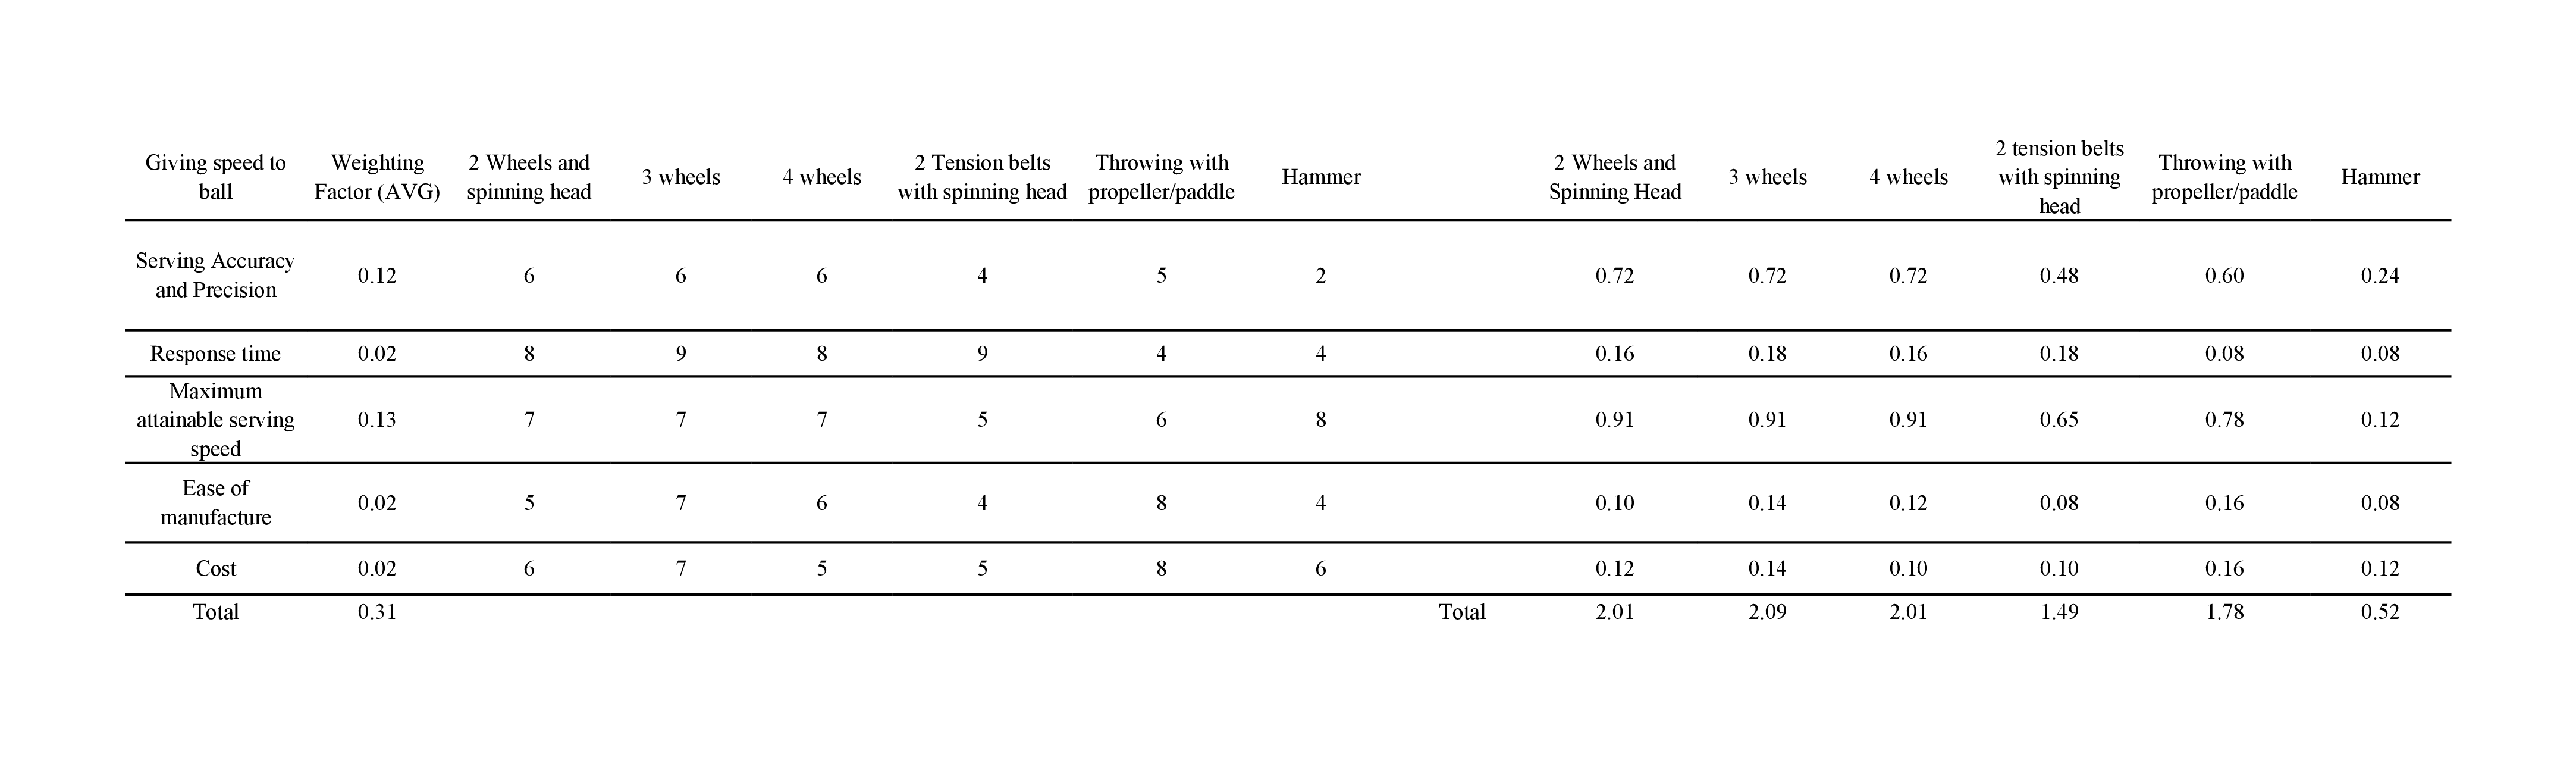
\includegraphics[width=1\textwidth]{Decision matrices/speed.png}
    \caption{Giving speed to the ball}
\end{figure}

Similarly, three alternatives were considered for controlling the speed of the balls. As was the case in controlling spin, BLDC motors were identified as the optimal solution due to their superior accuracy, precision, and ability to deliver higher maximum speeds.
\begin{figure}[H]
    \centering
    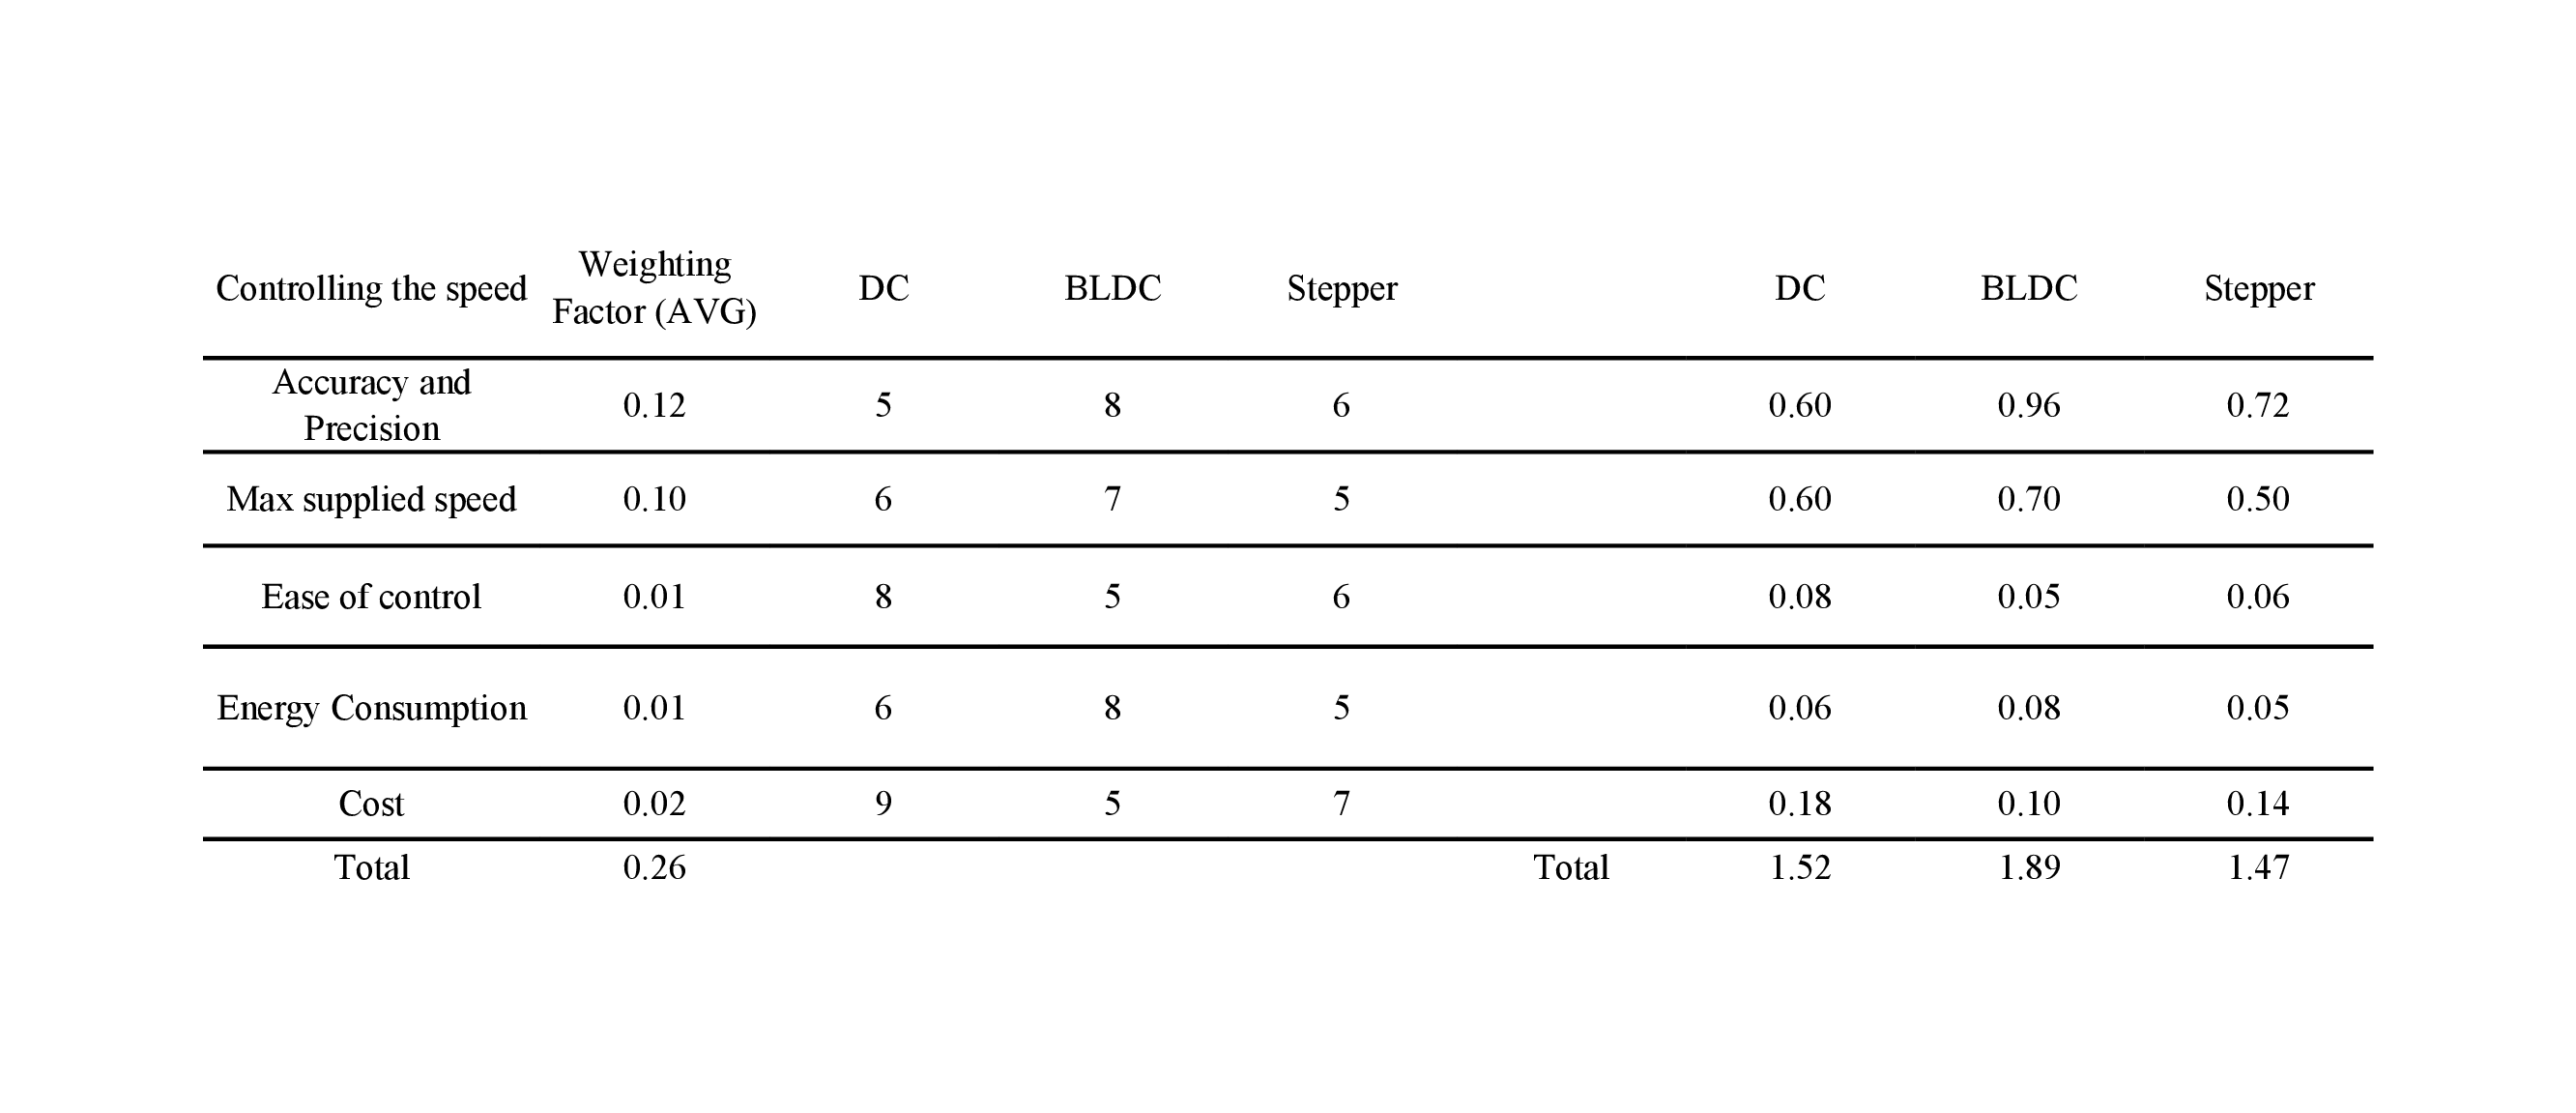
\includegraphics[width=1\textwidth]{Decision matrices/controlling speed.png}
    \caption{Controlling the speed}
\end{figure}

Six different solutions were proposed for providing the yaw angle to the mechanism, as outlined in the morphological chart. Among these, the solution referred to as "Gear 1" was identified as the optimal choice based on the decision matrix evaluation. This solution was selected due to its above-average performance across all criteria, making it the most balanced and effective option overall.

\begin{figure}[H]
    \centering
    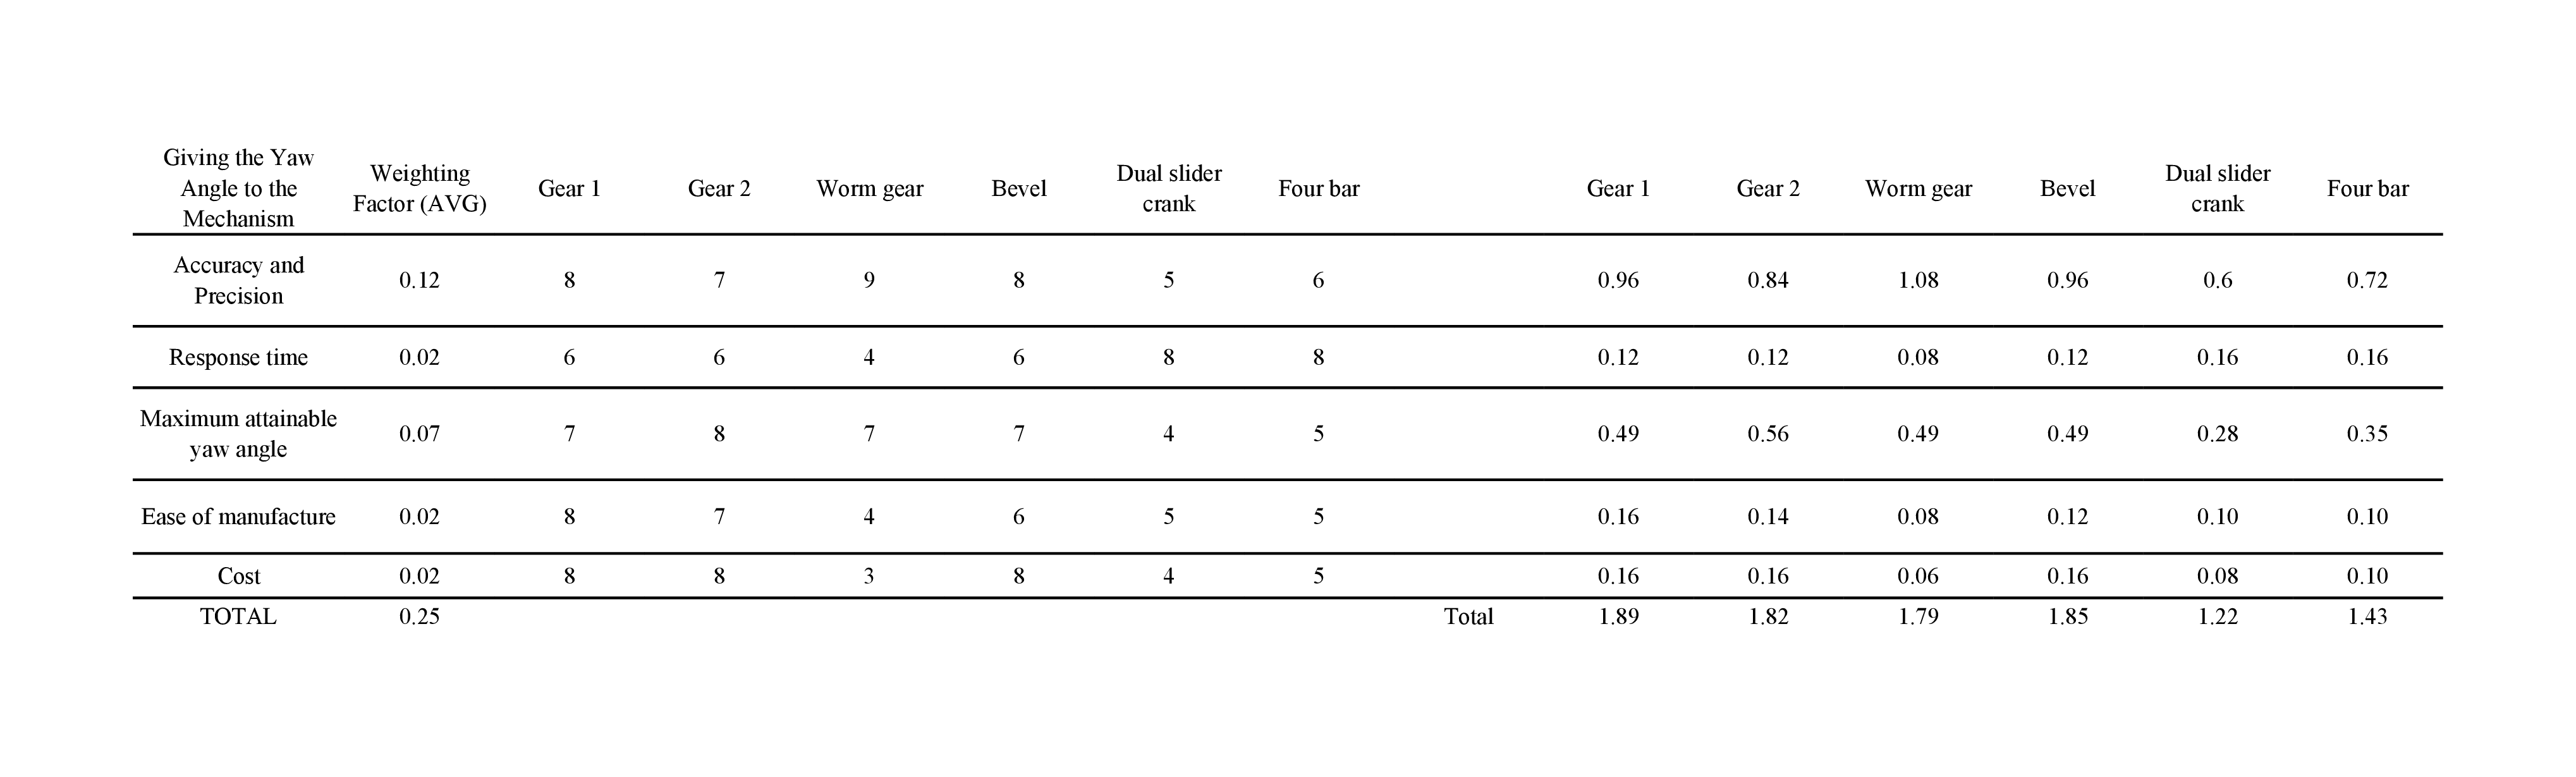
\includegraphics[width=1\textwidth]{Decision matrices/yaw.png}
    \caption{Giving yaw angle to the launching mechanism}
\end{figure}

For controlling the yaw angle, three motor alternatives were considered: servo, stepper, and DC with encoder. Based on the decision matrix evaluation, the servo motor was identified as the optimal solution. Its better accuracy and precision, along with its favorable cost, were key factors that made it the best choice for this application.

\begin{figure}[H]
    \centering
    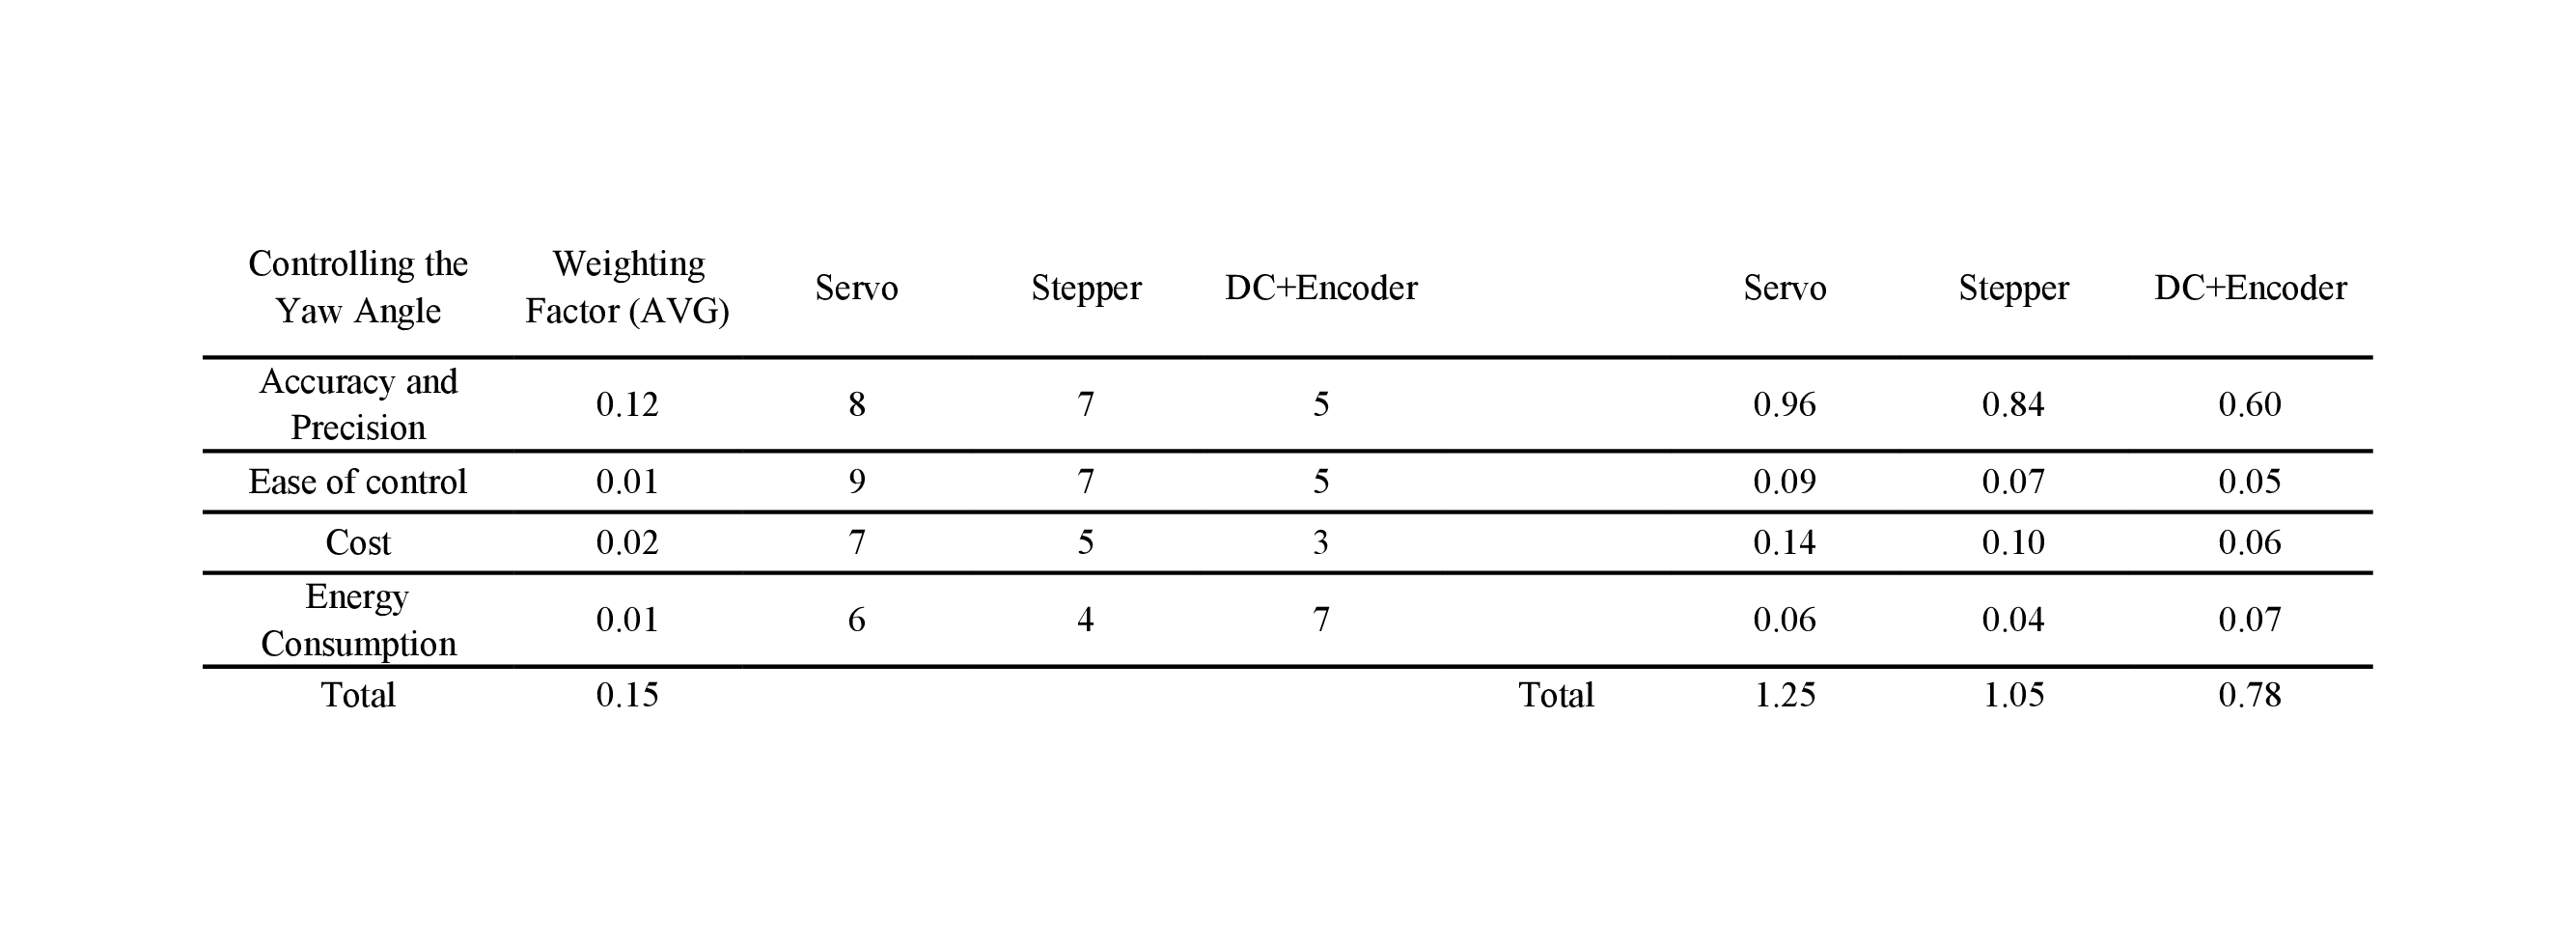
\includegraphics[width=1\textwidth]{Decision matrices/controlling yaw.png}
    \caption{Controlling the yaw angle}
\end{figure}

Six different solutions were proposed to give the pitch angle and, among them, the gear alternative was identified as the optimal solution. This choice was made based on its above-average performance across all criteria, making it the most suitable option to achieve the desired pitch angle.

\begin{figure}[H]
    \centering
    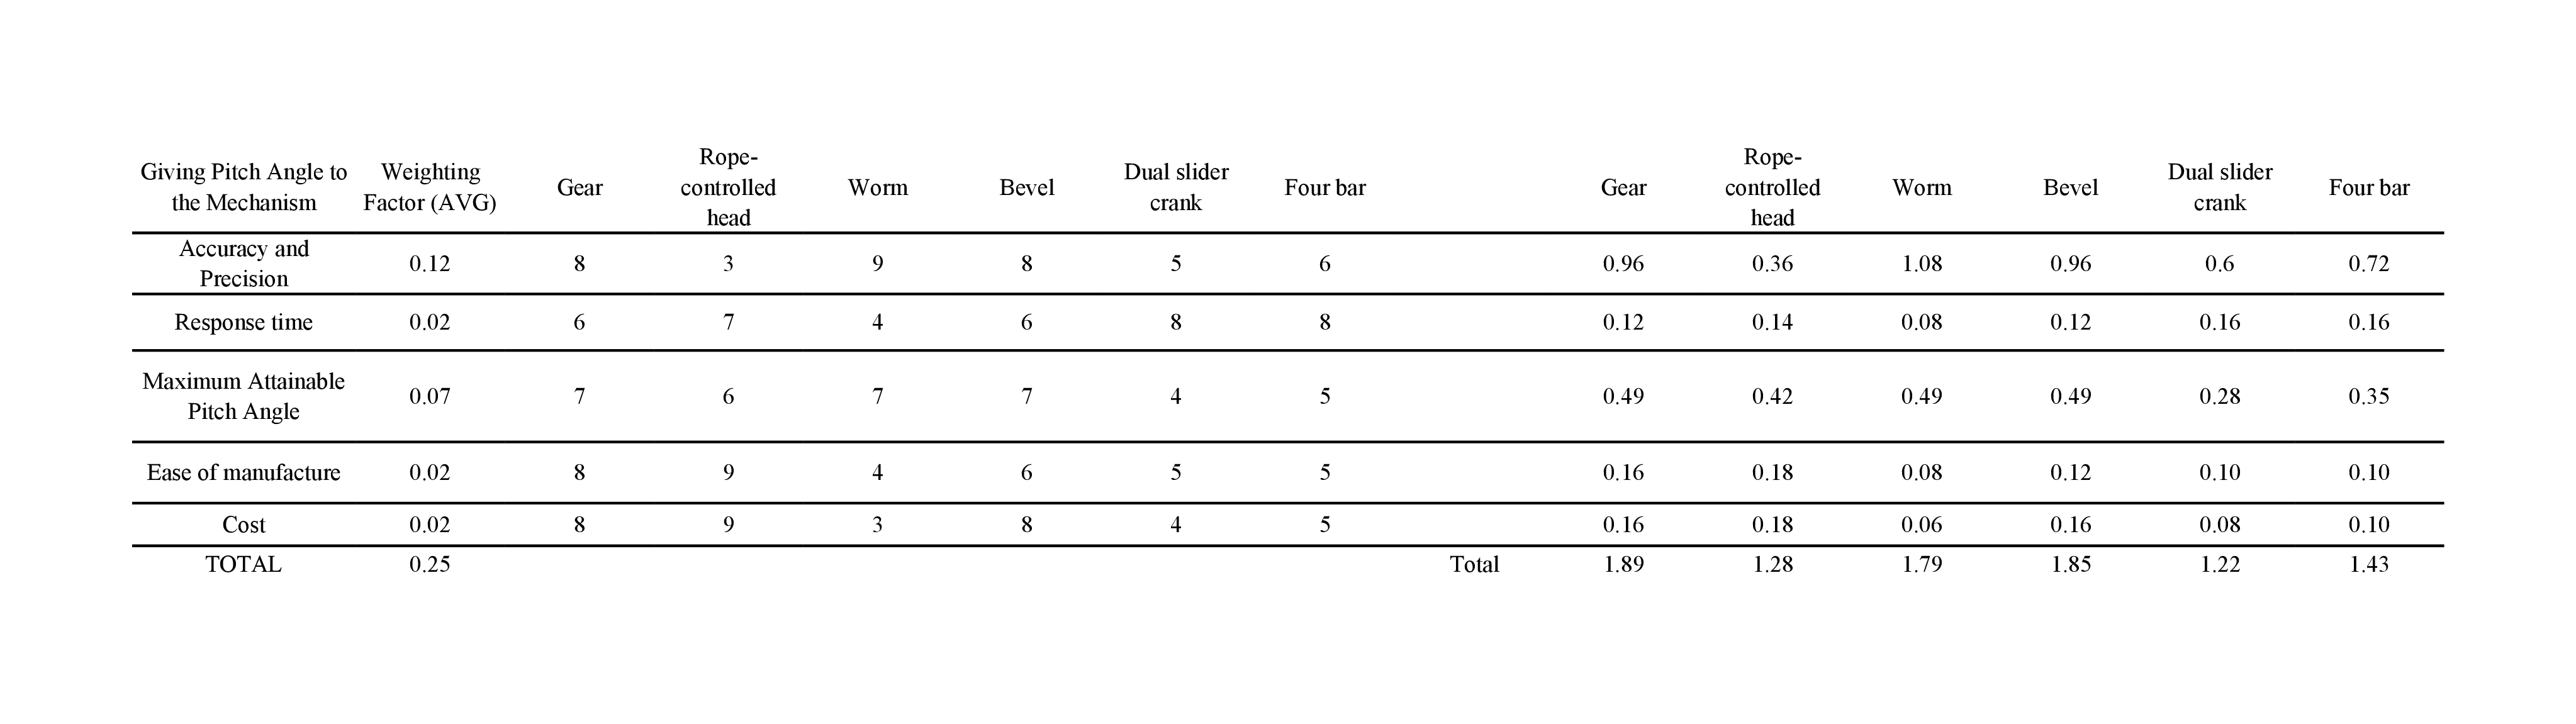
\includegraphics[width=1\textwidth]{Decision matrices/pitch.png}
    \caption{Giving pitch angle to the launching mechanism}
\end{figure}

For controlling the pitch angle, the same three alternatives as controlling the yaw angle were considered. Based on the evaluation of the decision matrix, the servomotor was identified as the optimal solution, similar to the selection to control the yaw angle.

\begin{figure}[H]
    \centering
    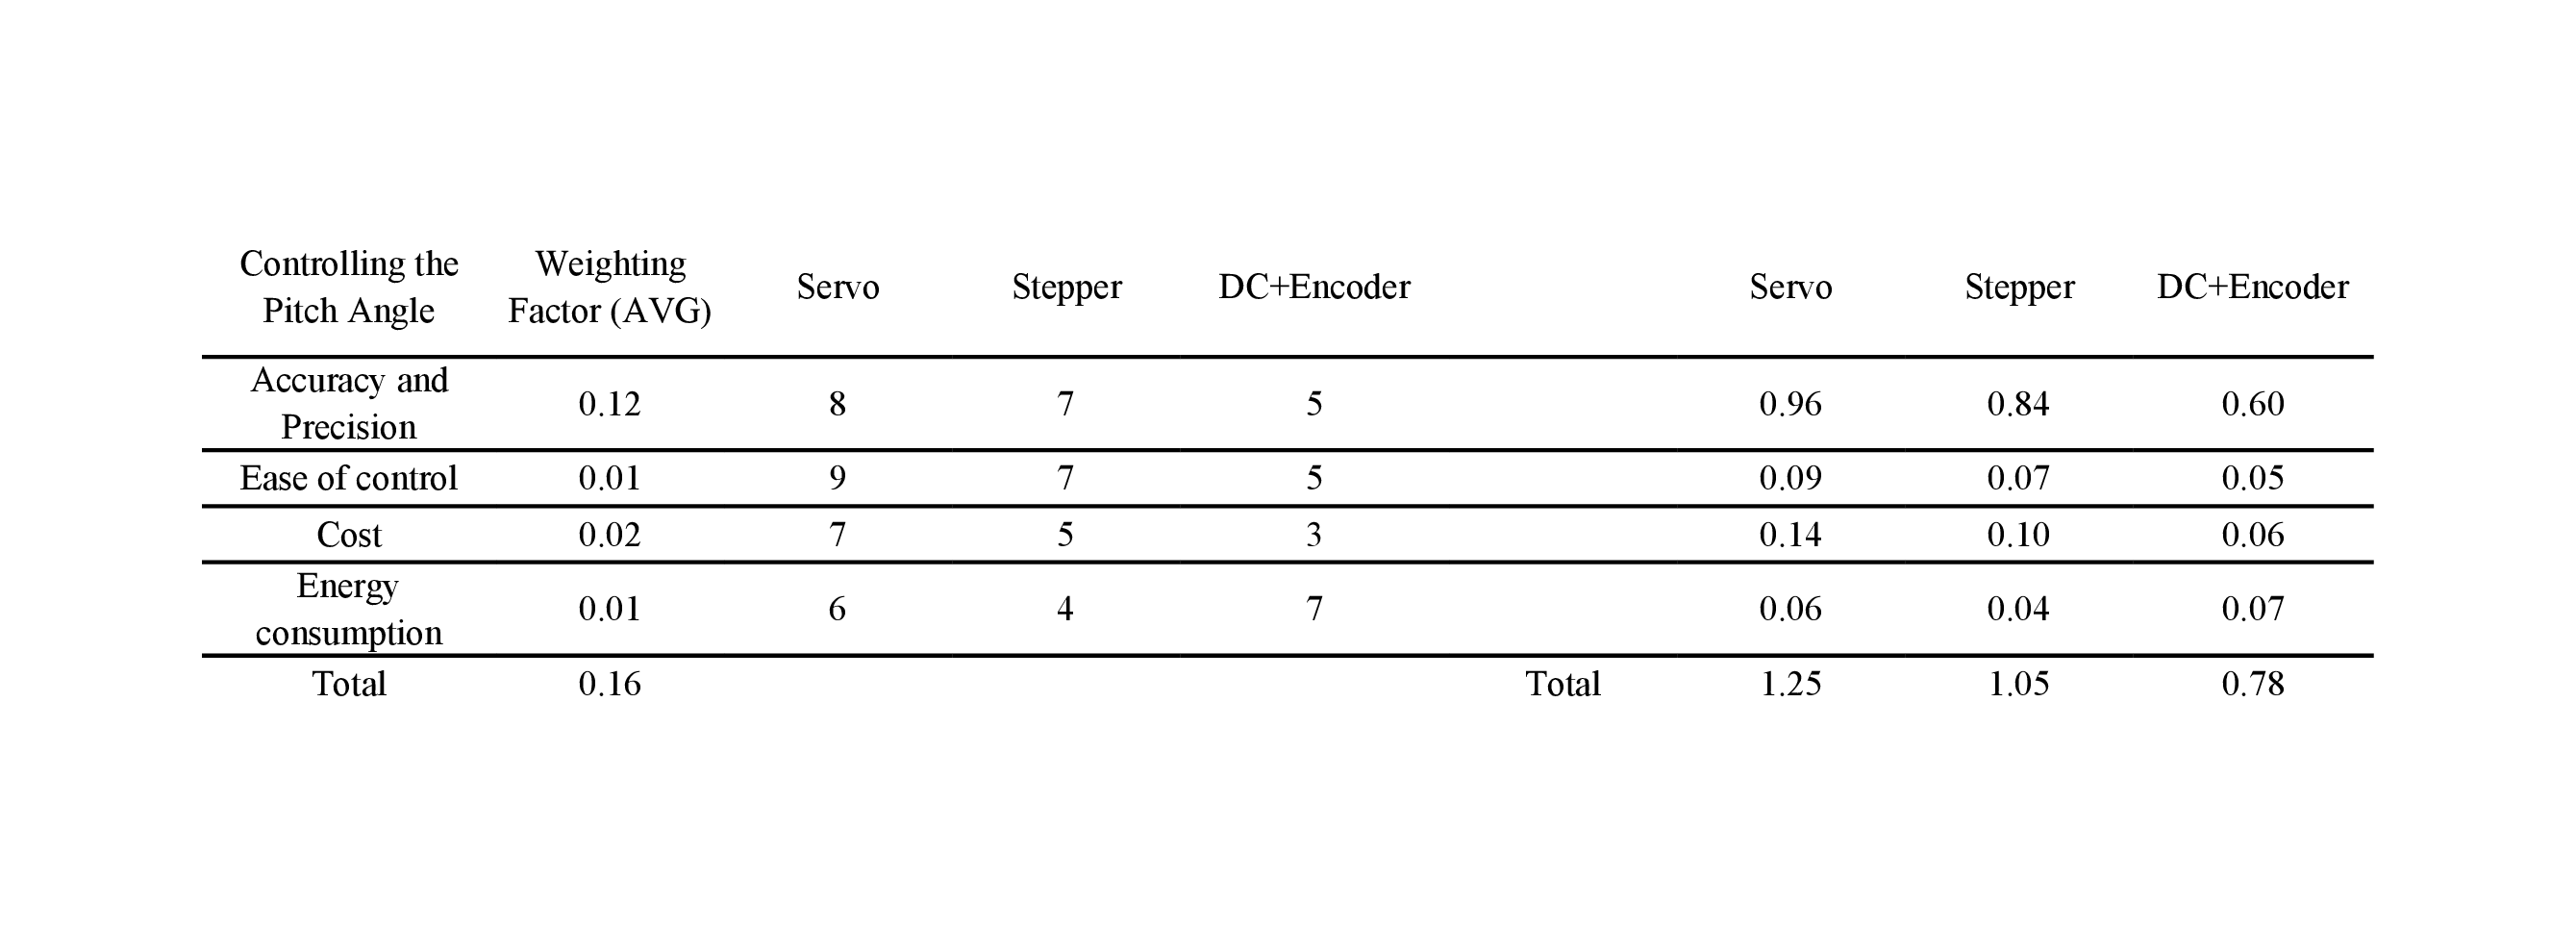
\includegraphics[width=1\textwidth]{Decision matrices/controlling pitch.png}
    \caption{Controlling the pitch angle}
\end{figure}

For accepting frequency information from the user, four alternatives were considered: integrated controller, IR remote, mobile, and wired remote. Based on the decision matrix evaluation, the integrated controller was identified as the optimal solution. Its advantages in terms of cost and ease of manufacture made it the best choice for this application.

\begin{figure}[H]
    \centering
    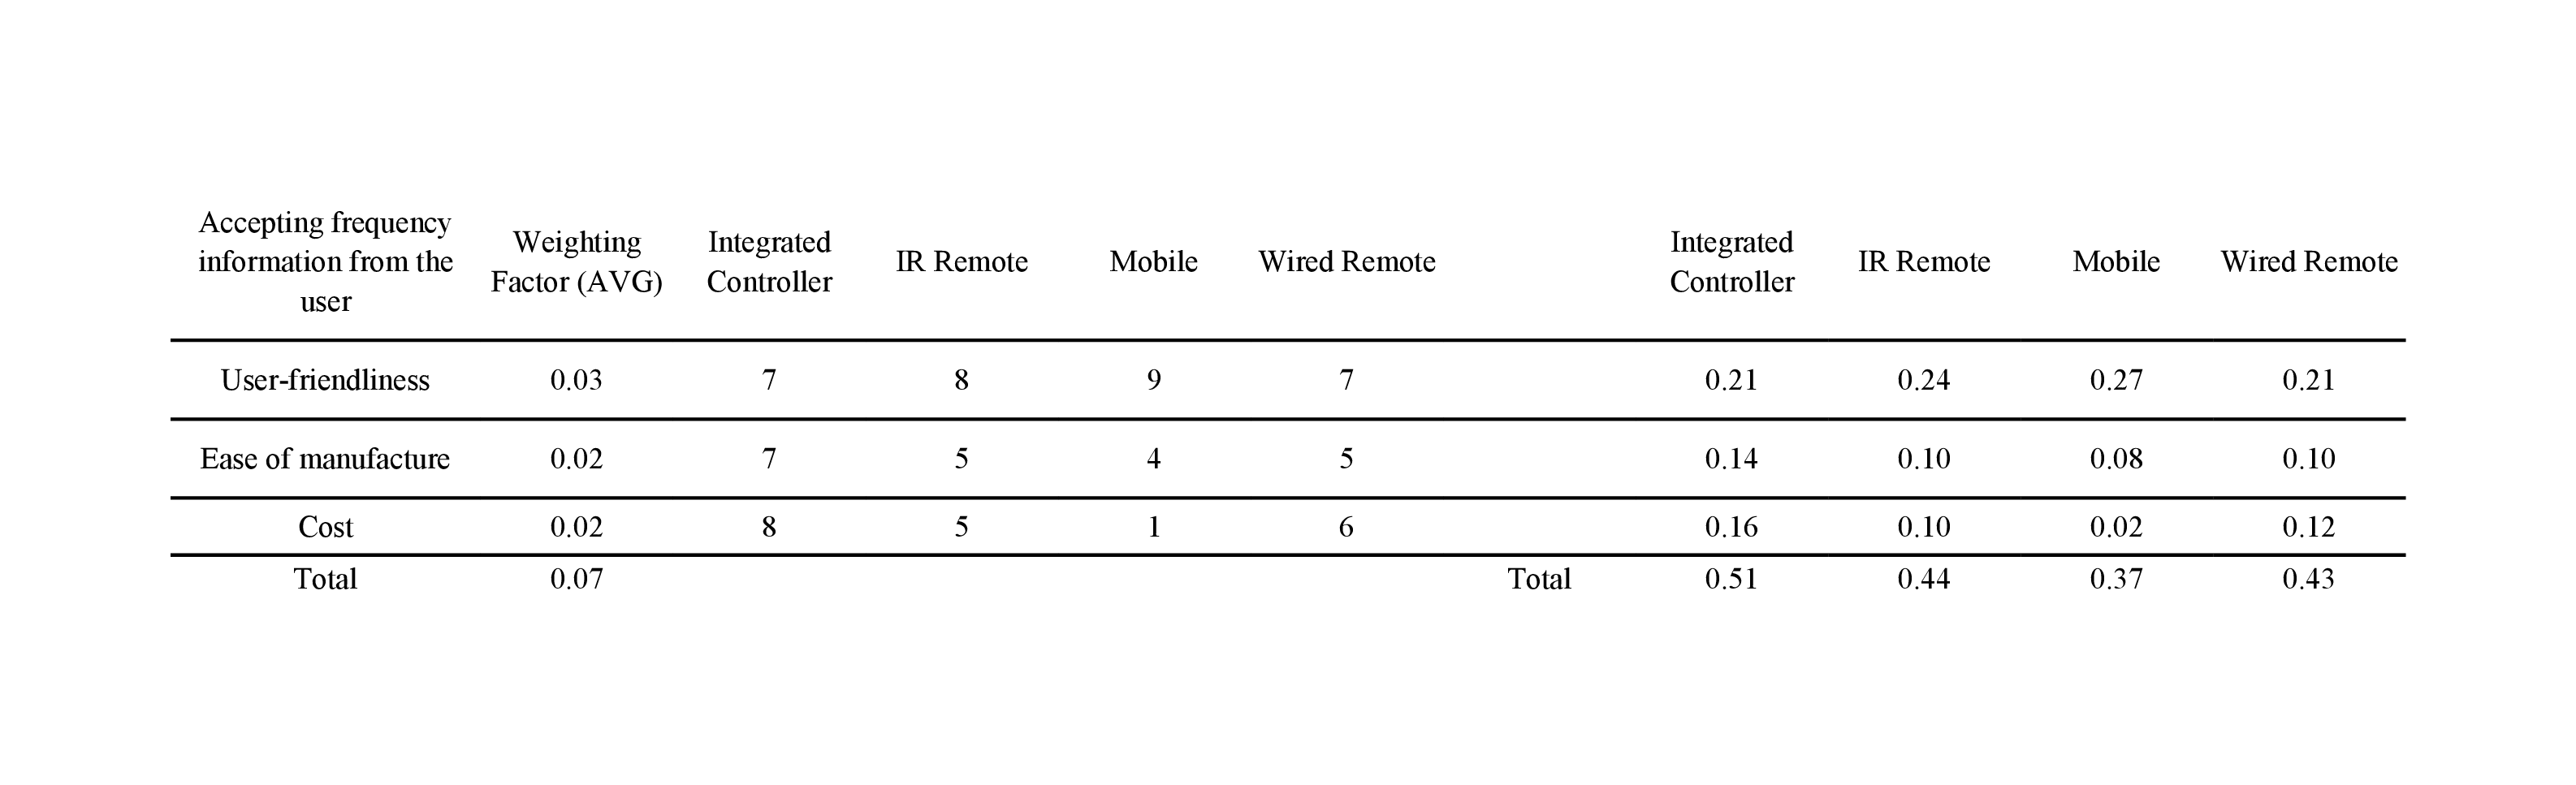
\includegraphics[width=1\textwidth]{Decision matrices/accept frequency.png}
    \caption{Accepting frequency information from the user}
\end{figure}

For accepting numerical information from the user, four alternatives were considered: potentiometer, encoder, touch screen, and button. Based on the decision matrix evaluation, the button was identified as the optimal solution. Its cost-effectiveness made it the best choice for this application.

\begin{figure}[H]
    \centering
    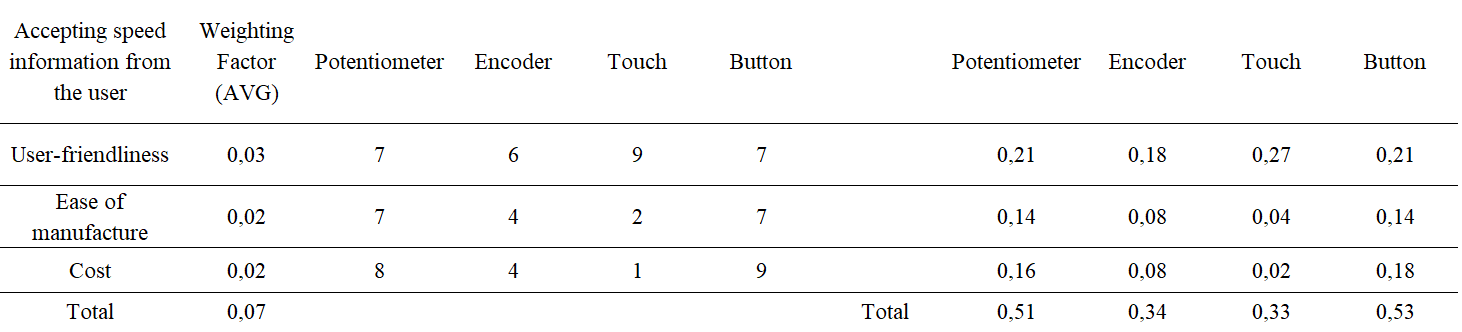
\includegraphics[width=1\textwidth]{Decision matrices/accept numerical.png}
    \caption{Accepting numerical information from the user}
\end{figure}

For accepting trajectory information from the user, the same four alternatives were considered. Similarly, the evaluation of the decision matrix identified the integrated controller as the optimal solution.

\begin{figure}[H]
    \centering
    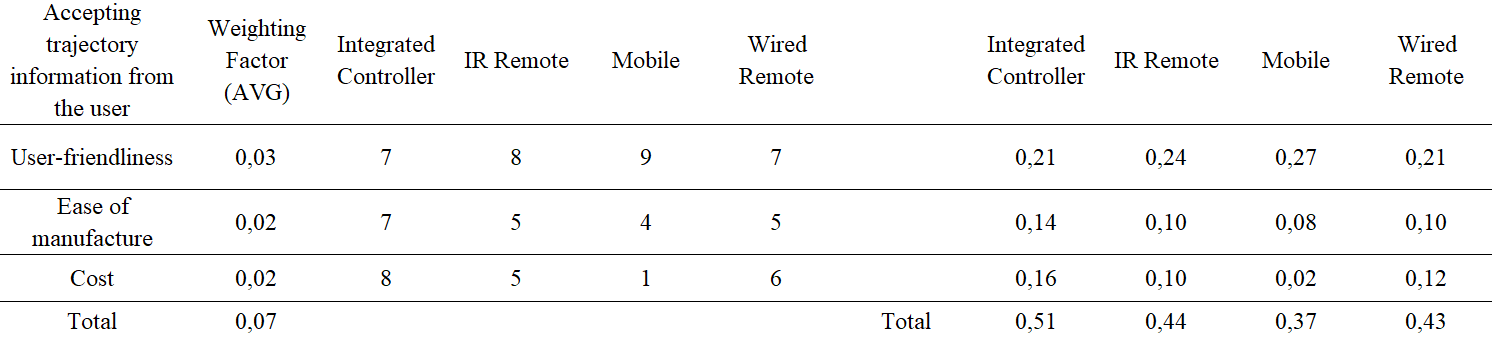
\includegraphics[width=1\textwidth]{Decision matrices/accept traj.png}
    \caption{Accepting trajectory information from the user}
\end{figure}


For allowing the user to position the device, five alternatives were considered: clamp, magnet, suction, rail, and wheel. Based on the decision matrix evaluation, the clamp was identified as the optimal solution. It demonstrated above-average performance across all criteria, making it the best choice for this application.

\begin{figure}[H]
    \centering
    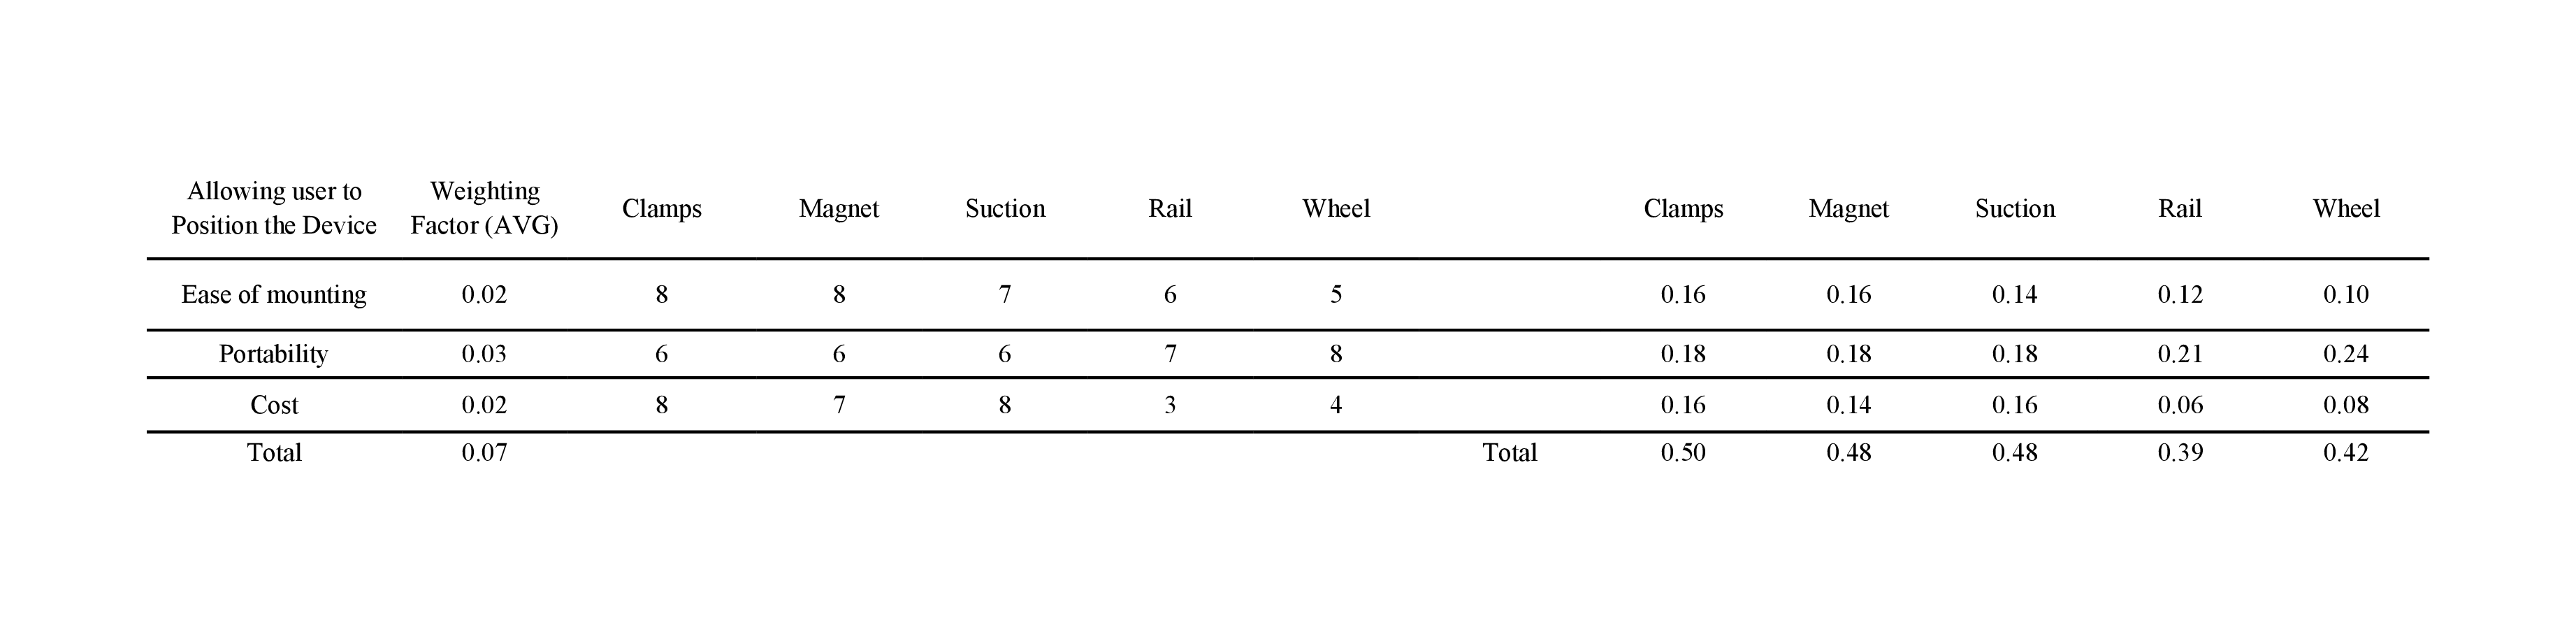
\includegraphics[width=1\textwidth]{Decision matrices/position device.png}
    \caption{Allowing the user to position the device}
\end{figure}

For preventing balls from escaping, three alternatives were considered: net, spherical wall, and wipers with net. Based on the decision matrix evaluation, the net was identified as the optimal solution. Its advantages in terms of portability, cost, and ease of manufacture made it the best choice for this application.

\begin{figure}[H]
    \centering
    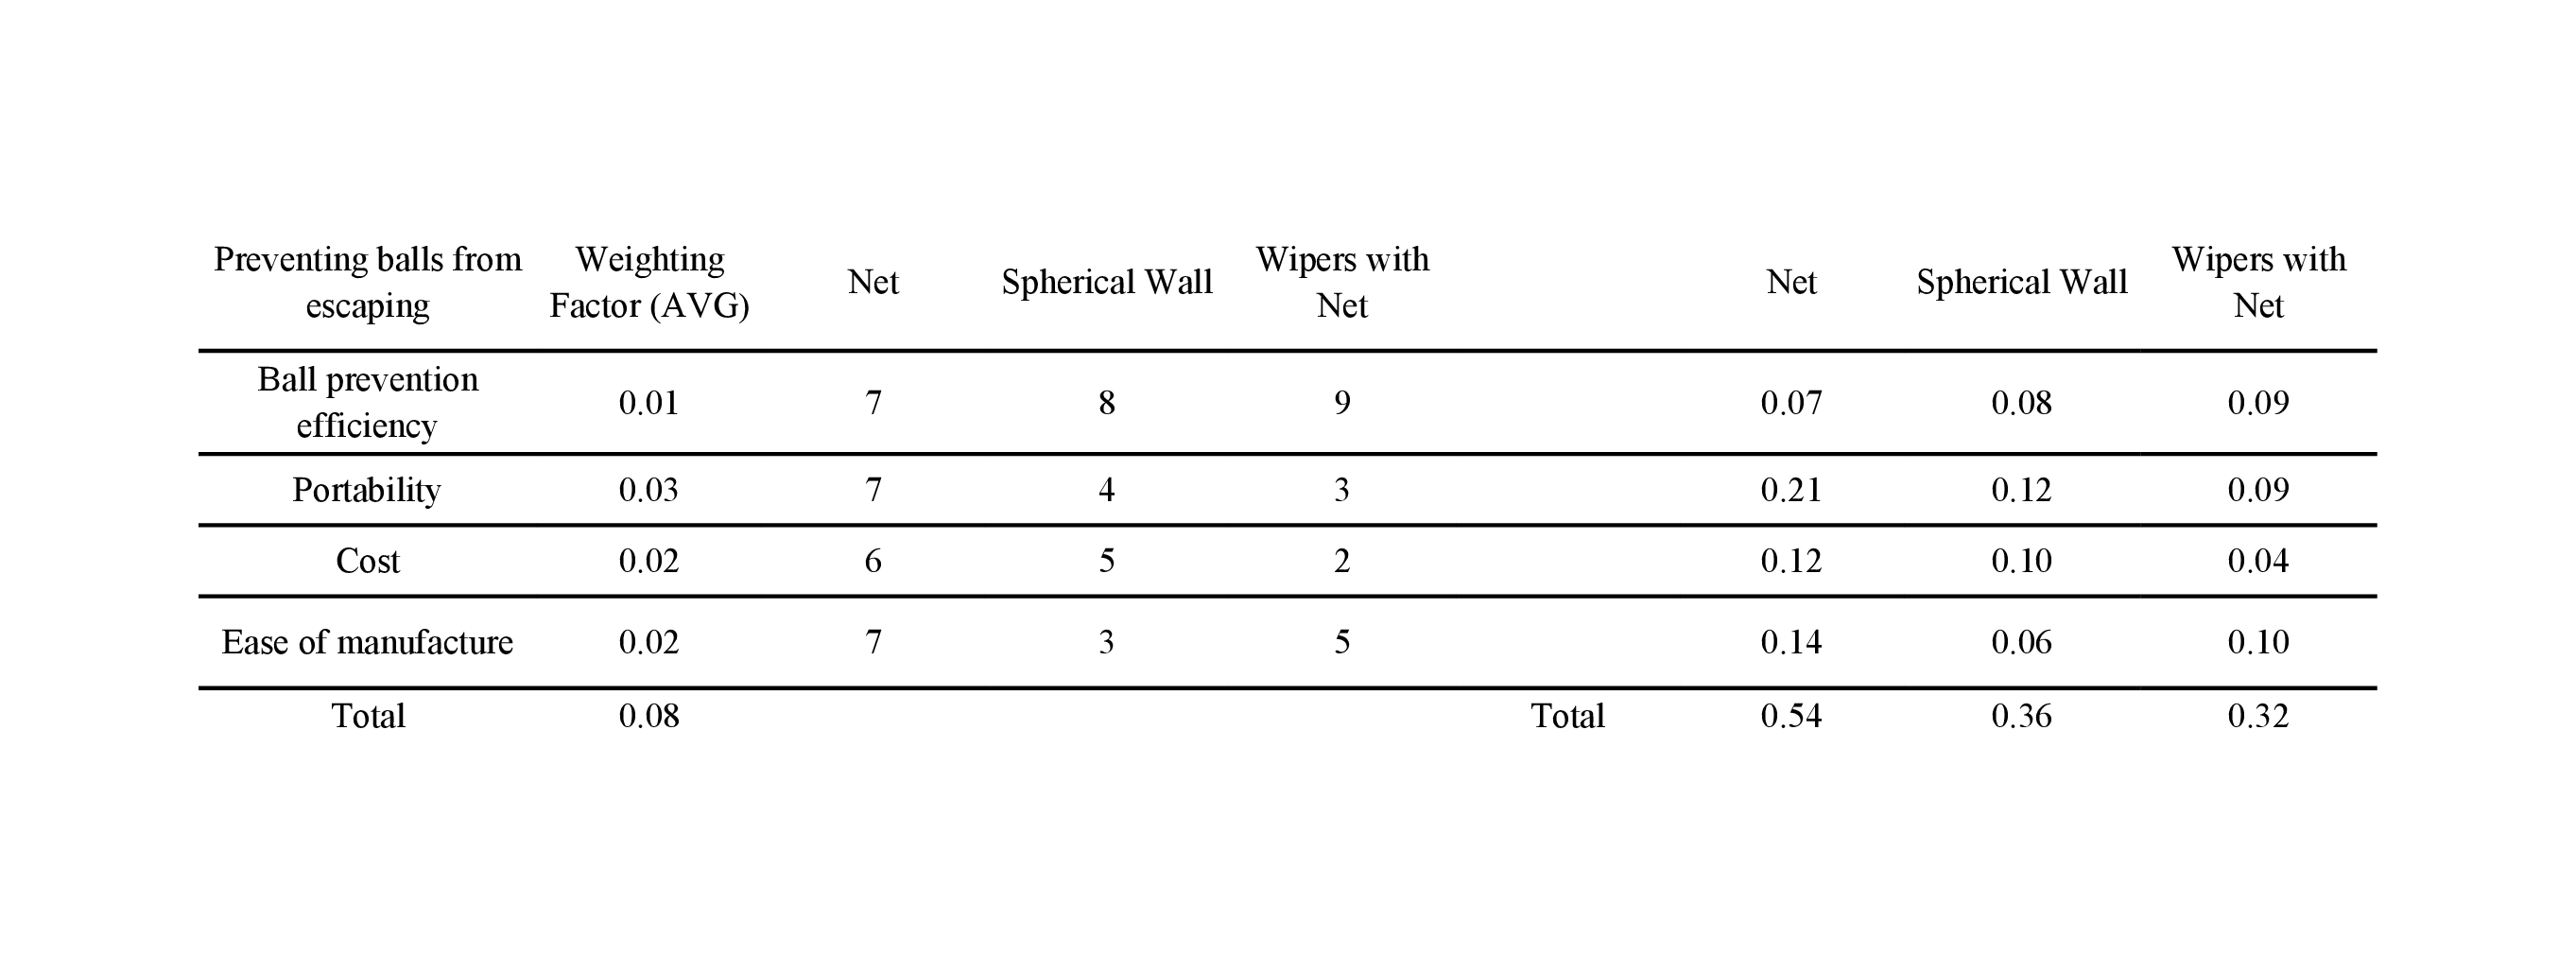
\includegraphics[width=1\textwidth]{Decision matrices/prevent escaping.png}
    \caption{Preventing balls from escaping}
\end{figure}

For storing the balls, four alternatives were considered: box, tunnel, groove, and gravity funnel. Based on the decision matrix evaluation, the groove was identified as the optimal solution. Its advantages in terms of capacity and portability made it the best choice for this application.

\begin{figure}[H]
    \centering
    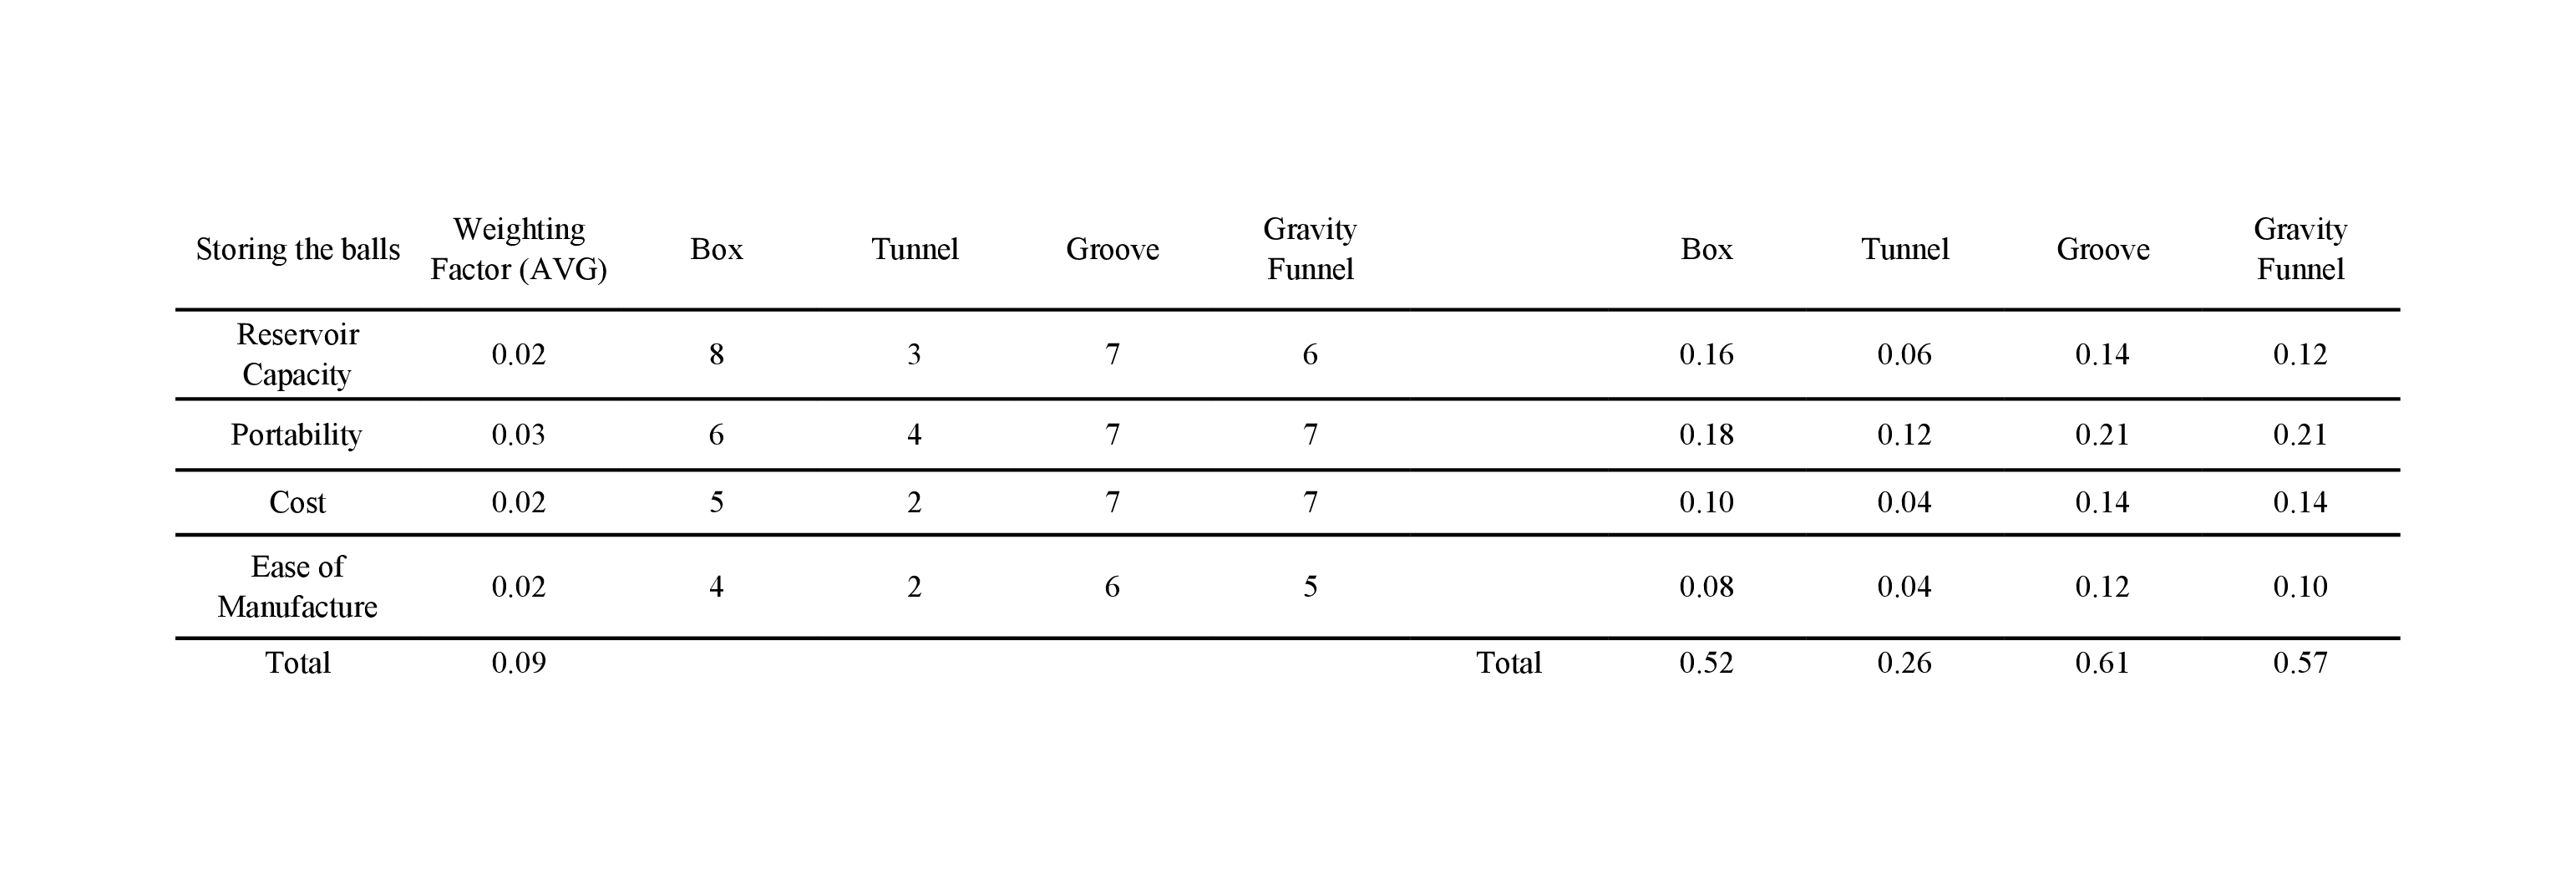
\includegraphics[width=1\textwidth]{Decision matrices/storing.png}
    \caption{Storing the balls}
\end{figure}
For transferring balls from storage, four alternatives were considered: Maltese wheel, spiral lift, translating box, and belt mechanism. Based on the decision matrix evaluation, the Maltese wheel was identified as the optimal solution. It demonstrated the best overall performance across all criteria, making it the most suitable choice for this application.

\begin{figure}[H]
    \centering
    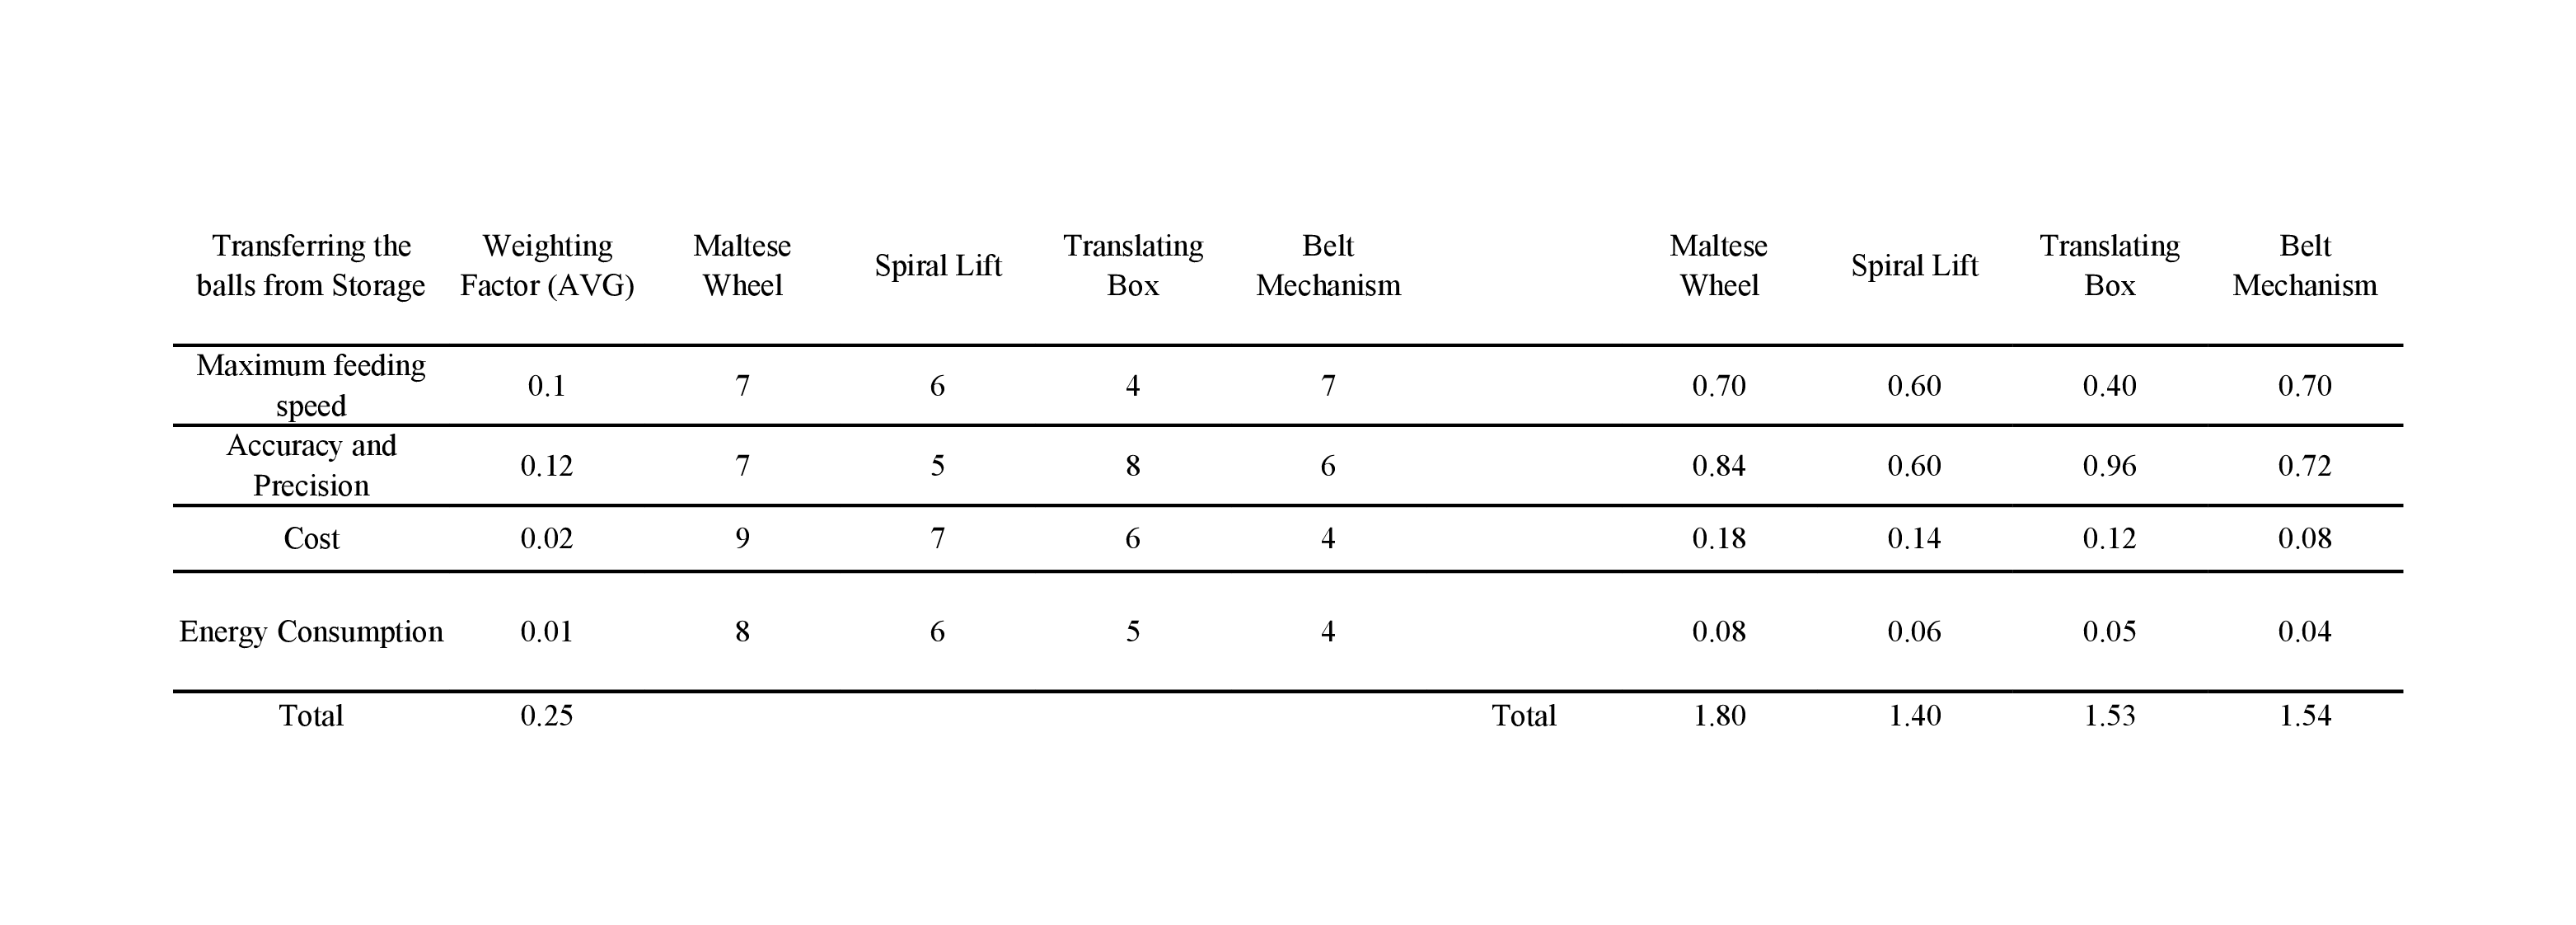
\includegraphics[width=1\textwidth]{Decision matrices/transfer from storage.png}
    \caption{Transferring the balls from  the storage} 
\end{figure}

For controlling the ball feed for storage, three alternatives were considered: stepper, DC, and DC with encoder. Based on the decision matrix evaluation, the stepper motor was identified as the optimal solution. It demonstrated above-average performance across all criteria, making it the most suitable choice for this application.

\begin{figure}[H]
    \centering
    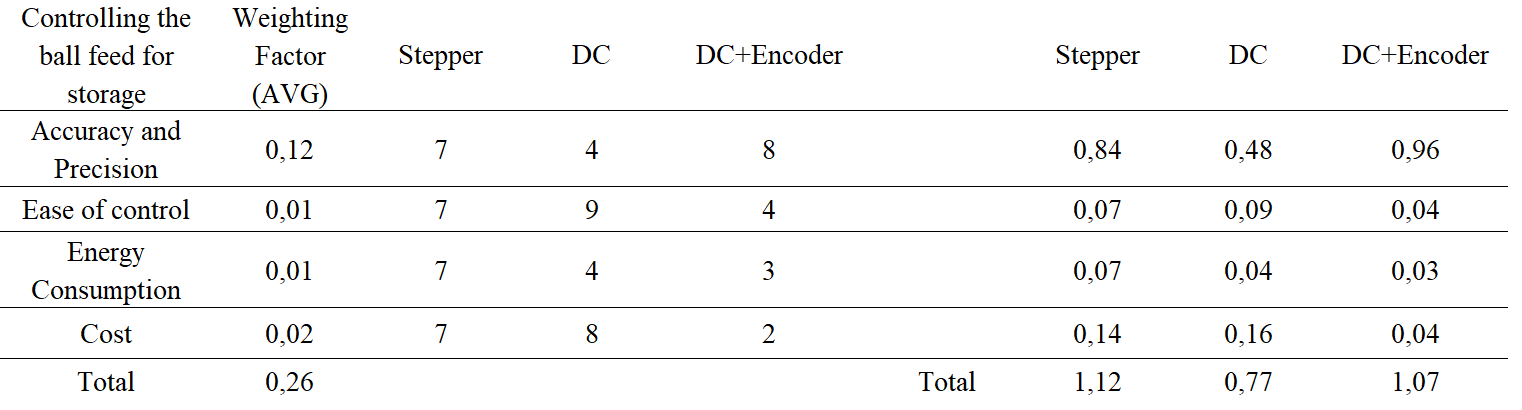
\includegraphics[width=1\textwidth]{Decision matrices/controlling ball feed for storage.png}
    \caption{Controlling the ball feed for storage}
\end{figure}

For transferring balls to launch, four alternatives were considered: Maltese wheel, spiral lift, rotating pusher, and belt mechanism. Based on the evaluation of the decision matrix, the Maltese wheel was identified as the optimal solution. It demonstrated above-average performance across all criteria, making it the most suitable choice for this application.

\begin{figure}[H]
    \centering
    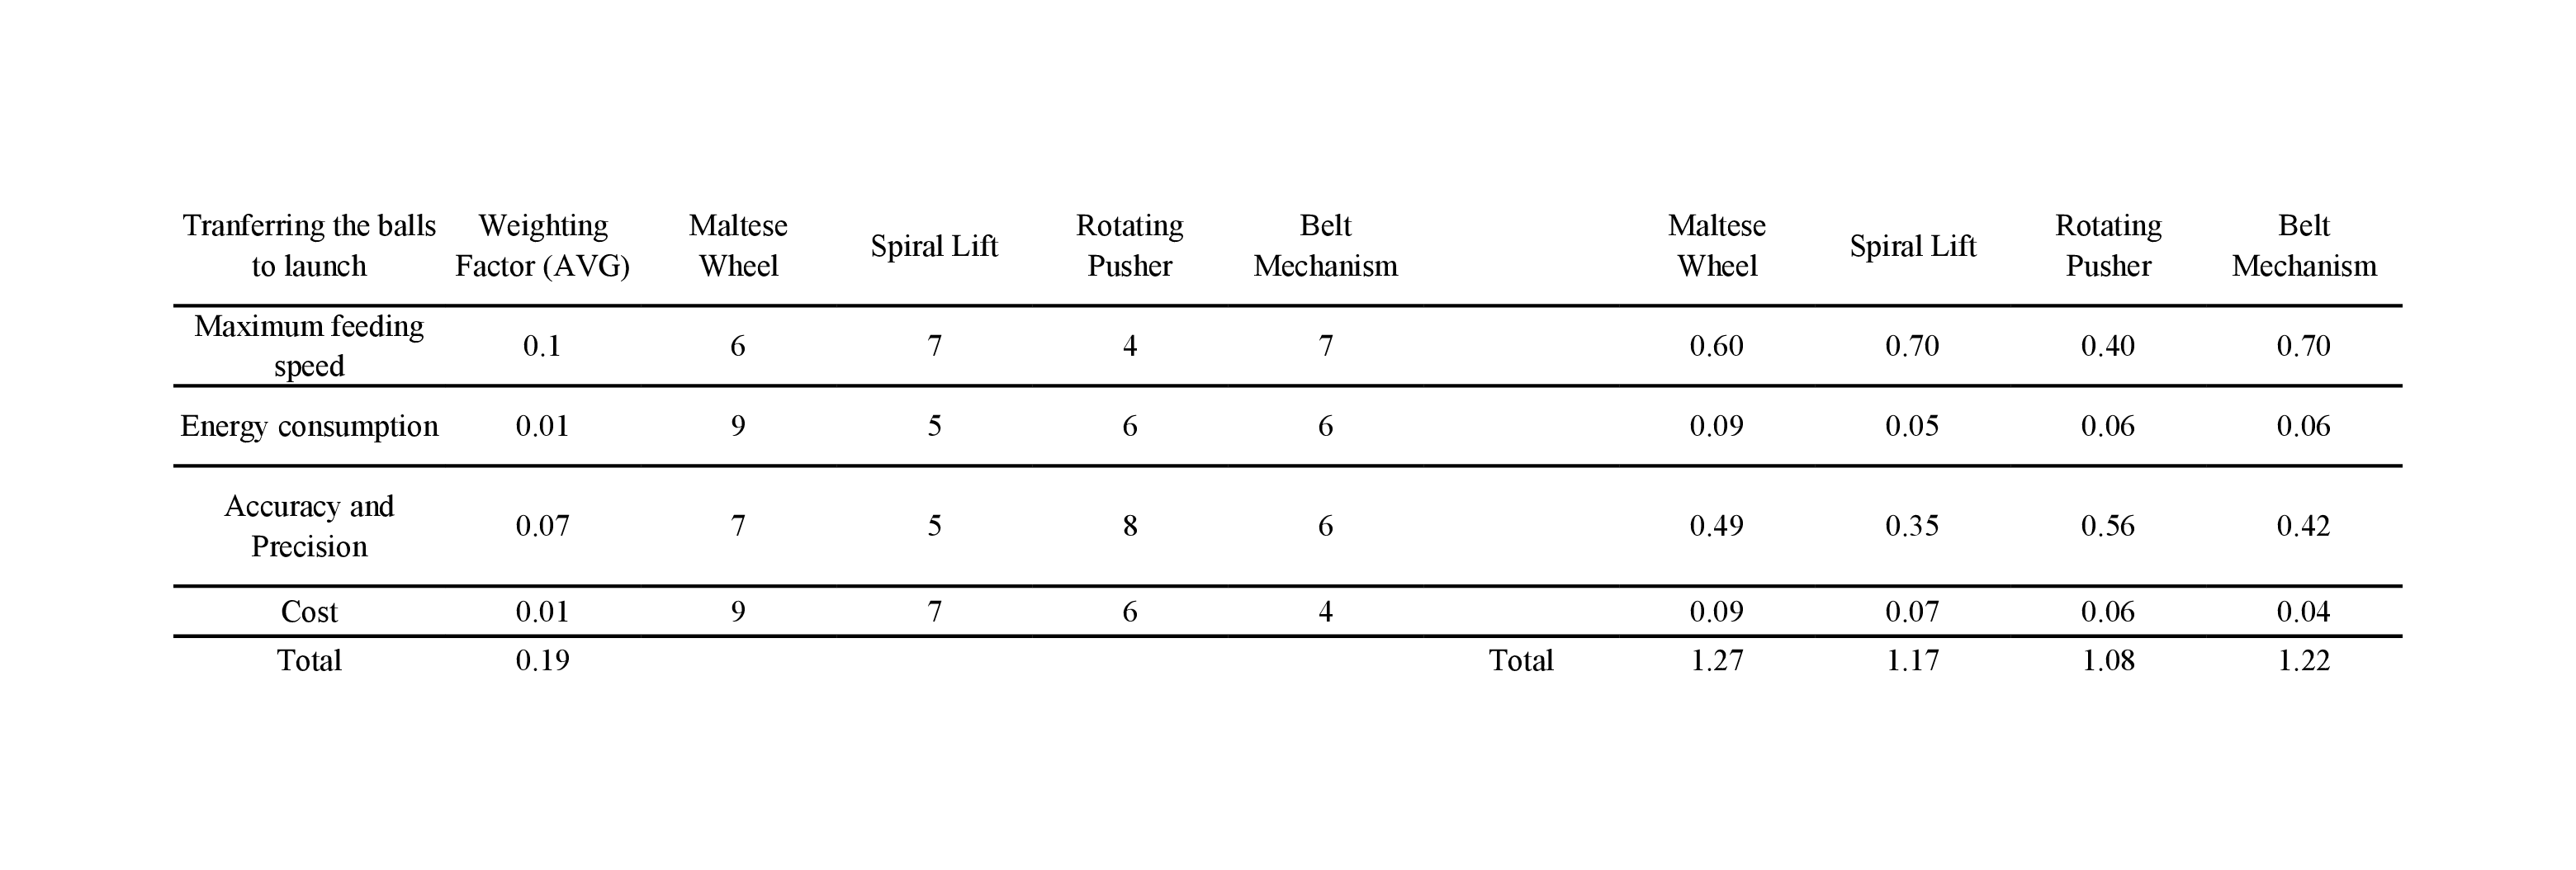
\includegraphics[width=1\textwidth]{Decision matrices/transfer to launch.png}
    \caption{Transferring the balls to launch }
\end{figure}

For controlling the ball feed for launching, three alternatives were considered. As was the case with ball feed control for storage, the stepper motor was identified as the optimal solution. It was selected as the optimal choice due to its overall performance, which satisfied expectations across all criteria.

\begin{figure}[H]
    \centering
    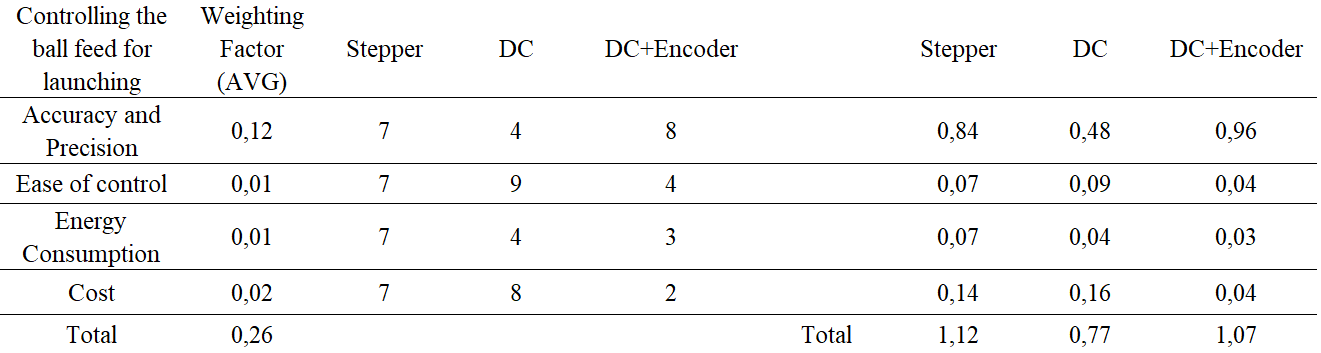
\includegraphics[width=1\textwidth]{Decision matrices/controlling ball feed for launching.png}
    \caption{Controlling the ball feed for launching}
\end{figure}

For the subfunction of giving the balls the desired frequency, six alternatives were considered. While the rotating pusher was identified as the optimal solution based on the decision matrix, particularly excelling in meeting the maximum attainable serving frequency criterion, the overall system design and integration with other subfunctions favored the use of the Maltese wheel. This approach ensures better compatibility and efficiency in the final design.

\begin{figure}[H]
    \centering
    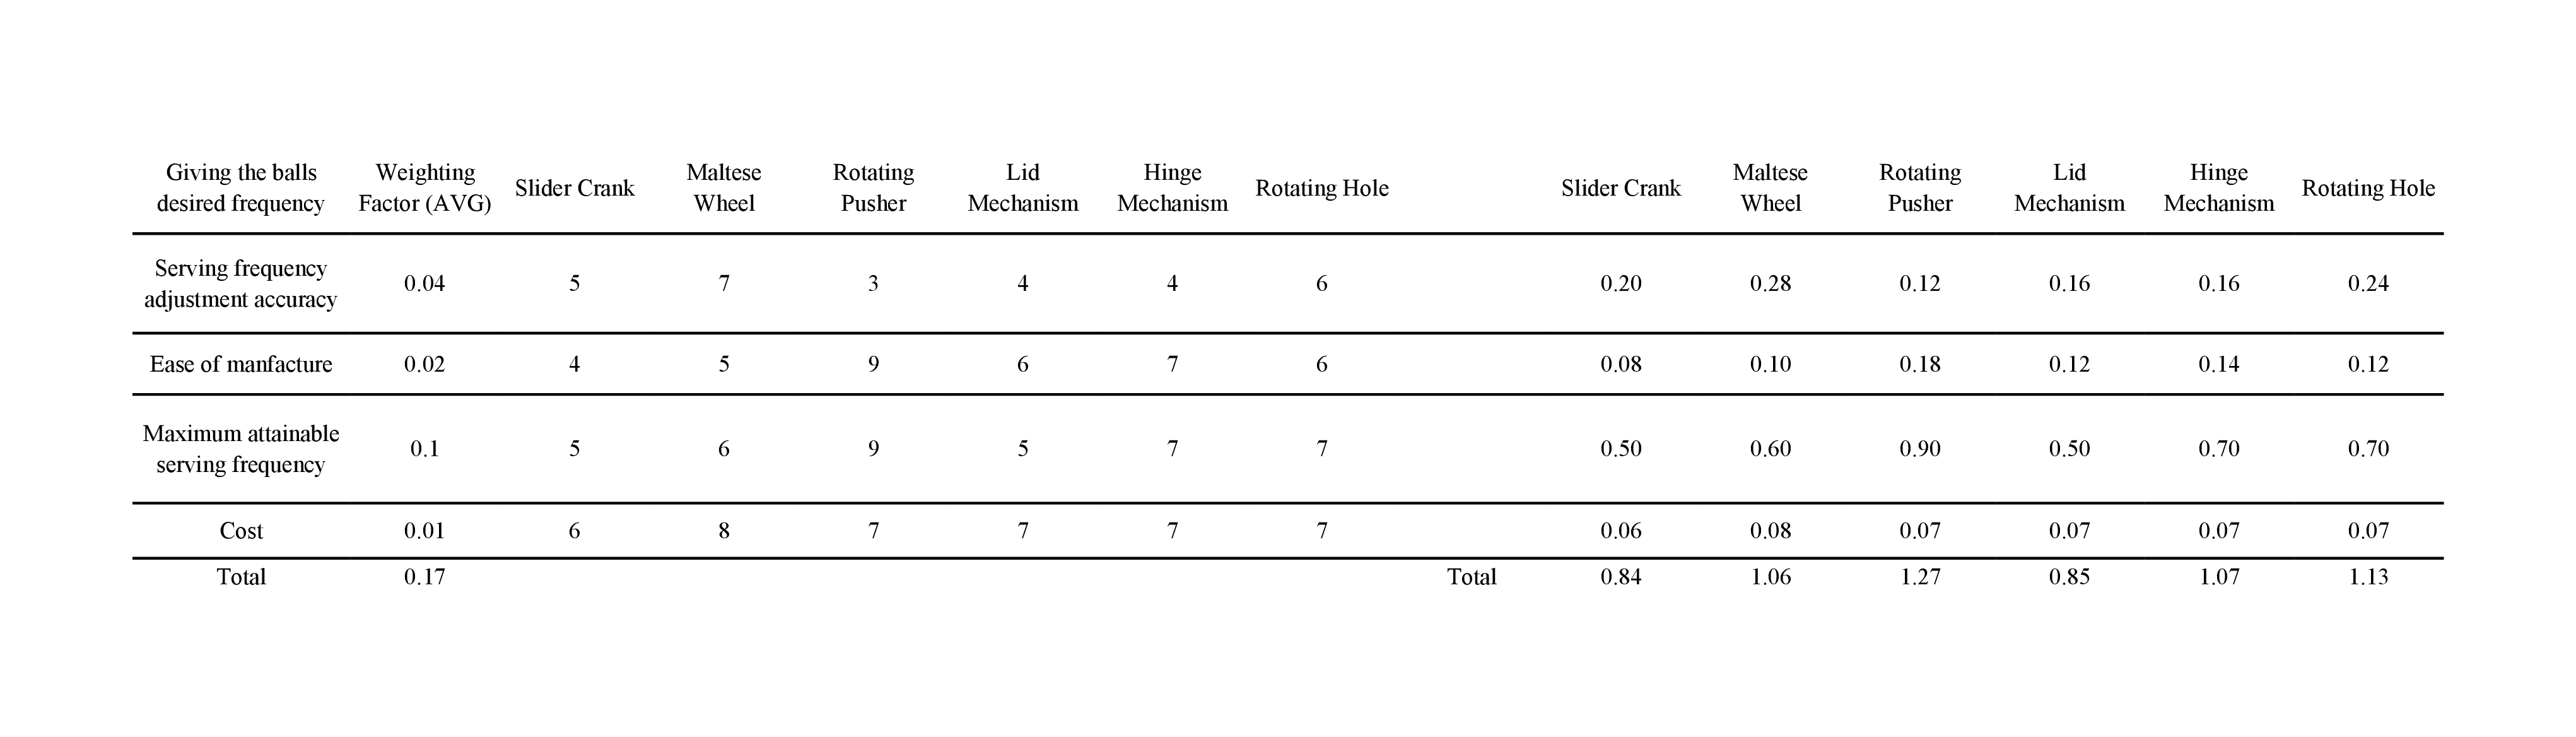
\includegraphics[width=1\textwidth]{Decision matrices/give frequency.png}
    \caption{ Giving the balls desired frequency}
\end{figure}

For the subfunction of controlling the ball frequency, three alternatives were evaluated. According to the decision matrix evaluation, the stepper motor was determined to be the optimal solution due to its better performance in terms of accuracy, precision, and cost-effectiveness, making it the most suitable choice for this application.

\begin{figure}[H]
    \centering
    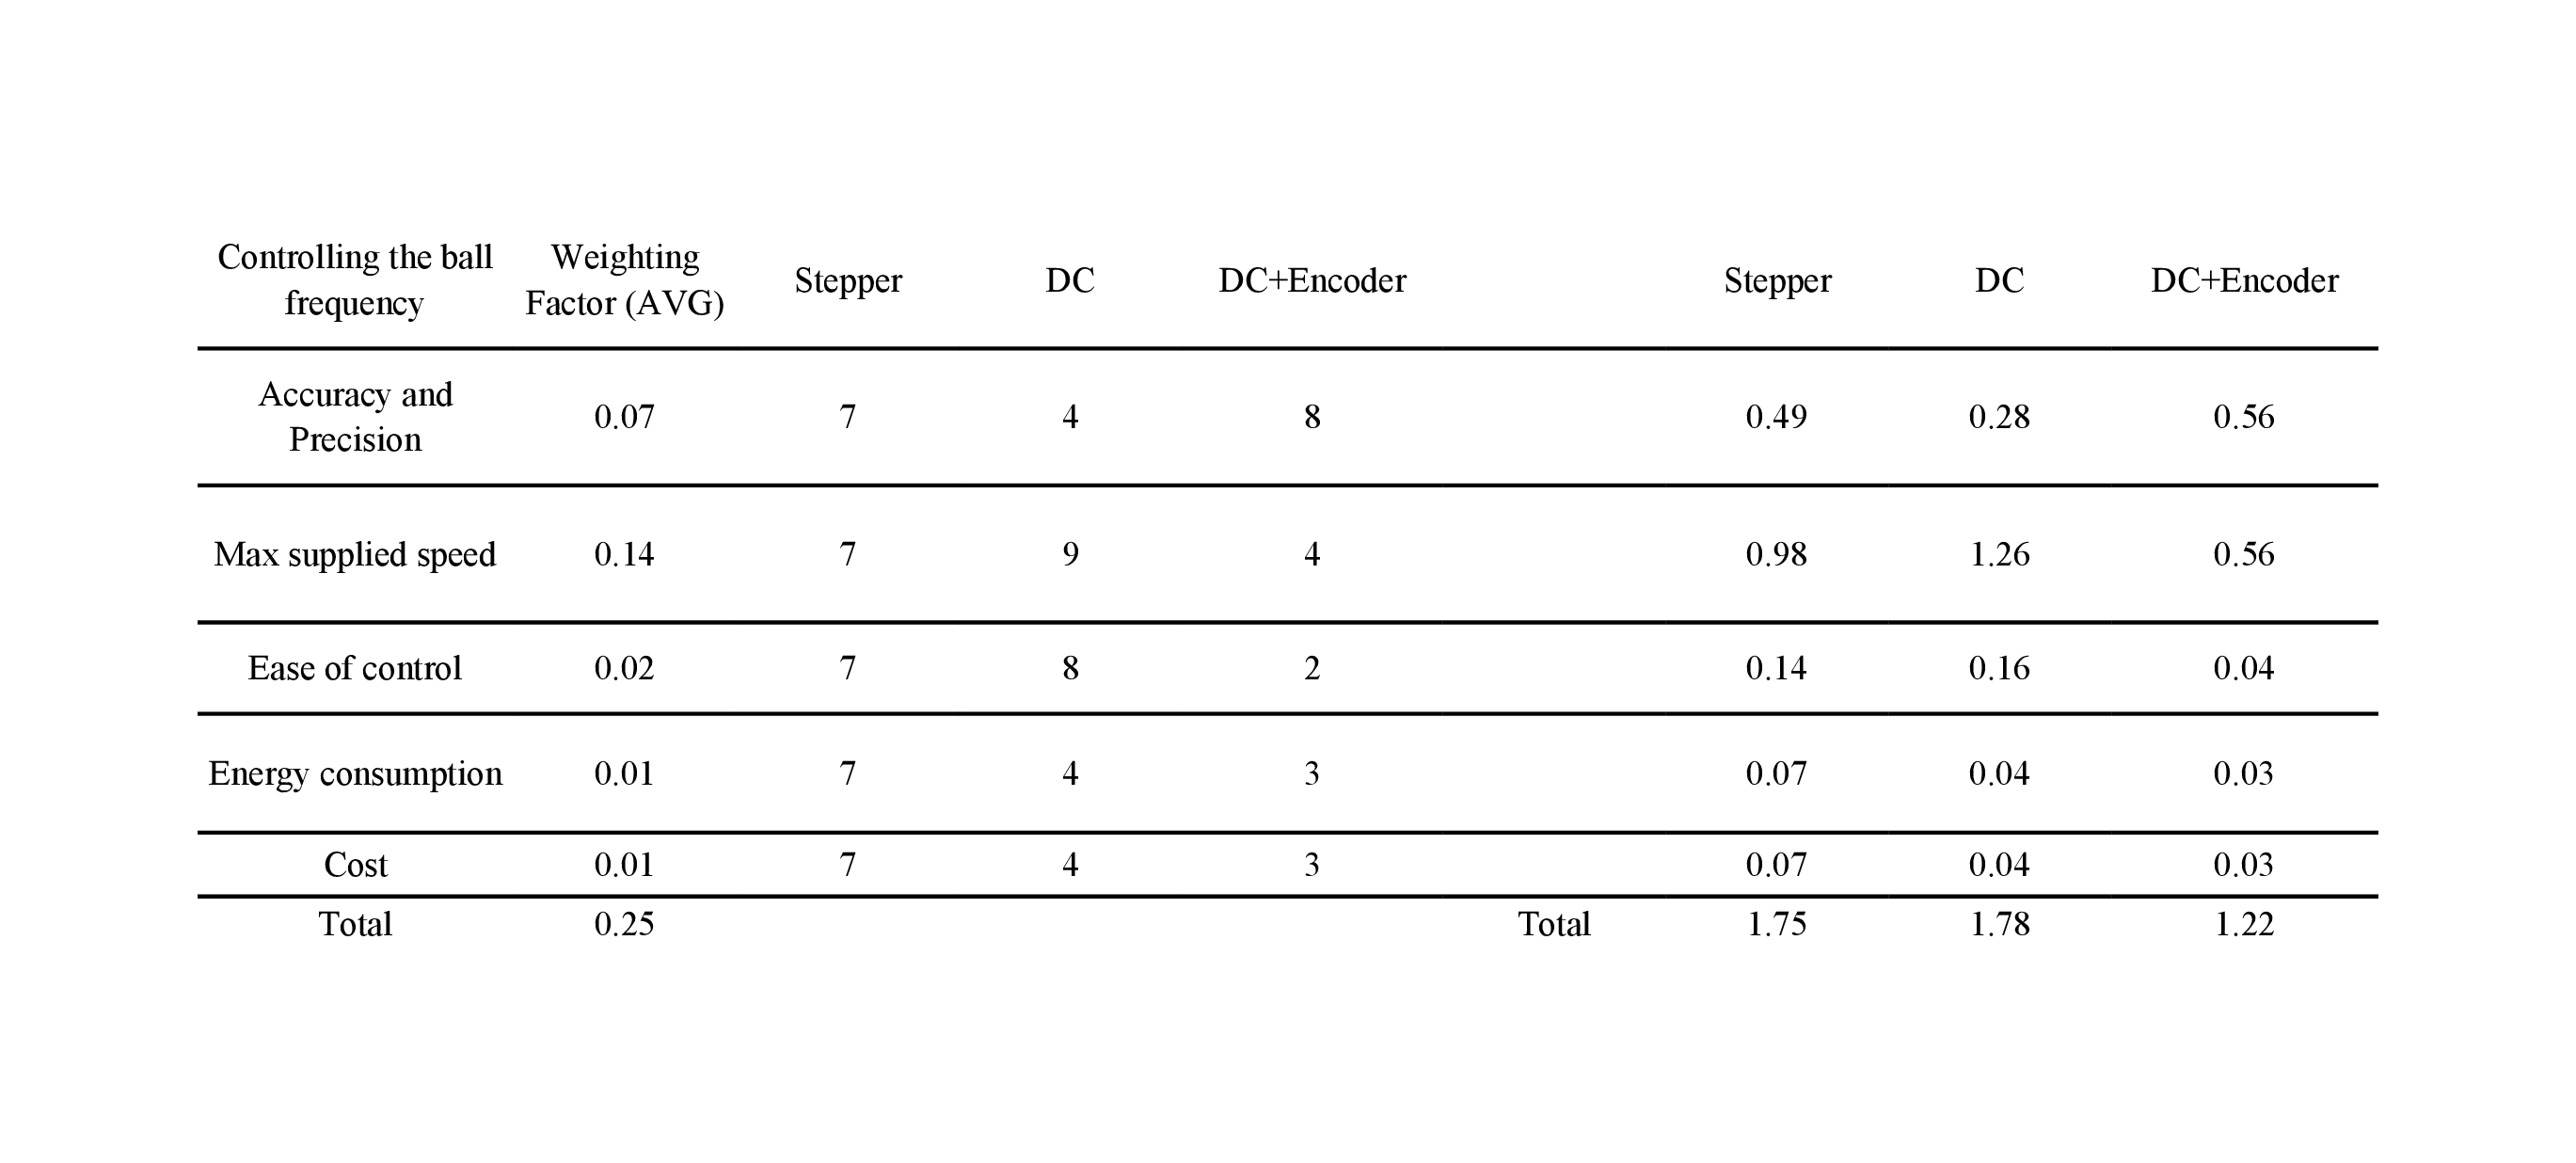
\includegraphics[width=1\textwidth]{Decision matrices/control frequency.png}
    \caption{Controlling the ball frequency}
\end{figure}


\begin{figure}[H]
    \centering
    \rotatebox{90}{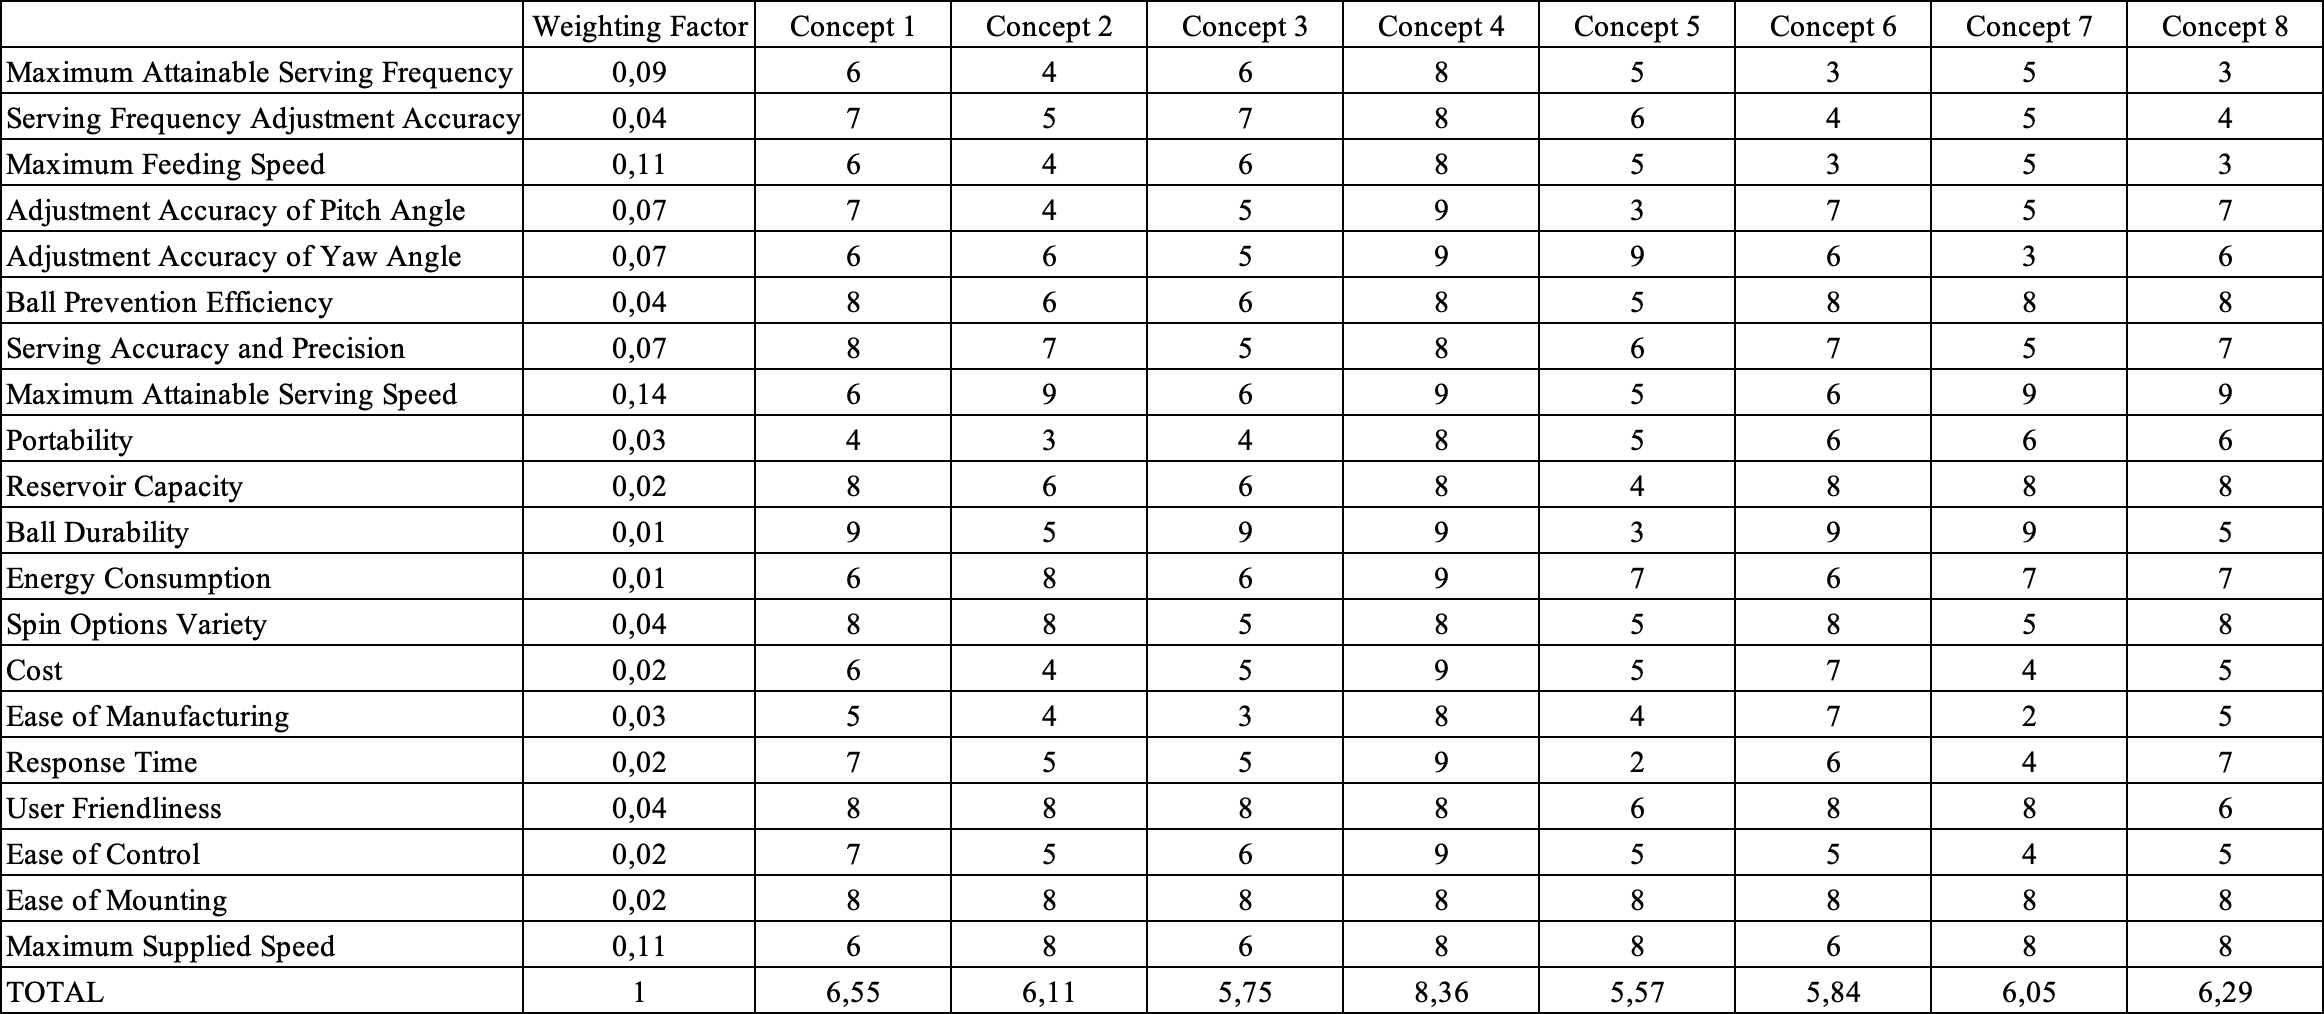
\includegraphics[width=\textheight]{obaa.jpg}}
    \caption{Concept Evaluation Normalized\cite{statista2024}}
    \label{fig:wholesales}
\end{figure}

\section{Best Concept}

\begin{minipage}{0.7\textwidth}

The best concept is chosen as Concept 4. Several factors determine this choice. Balls are stored in a groove structure (Figure ~\ref{fig:groove_mechanism}), ensuring organized storage and smooth feeding into the system. A net mechanism (Figure ~\ref{fig:net}) collects balls post-use and channels them back to the storage area, promoting recyclability and sustainability, enabling the user to have a continuous and favorable training experience. Possible ball leakage is prevented by using a net system to catch the balls and a groove mechanism for storage.

The balls are transferred from the storage to the launcher by a Maltese wheel (Figure ~\ref{fig:maltese}) through the "pushing effect" of consecutive balls, ensuring a smooth and consistent supply to the launcher. This Maltese wheel, operated by a stepper motor, facilitates precise ball direction toward the launch mechanism. The desired ball frequency is achieved by the rotation of the Maltese wheel, which determines the number of balls transferred per unit of time.

After the transfer process, a 3-wheel mechanism (Figure ~\ref{fig:3wheel}) launches the balls with the desired speed and spin. The speed is controlled by the linear speed of the wheels, which are driven by BLDC motors. For instance, if all three wheels rotate at the same speed (assuming equal dimensions), the ball is launched without spin. Conversely, a speed difference between the wheels imparts spin to the ball, such as top-spin, side-spin, or back-spin, depending on the faster wheel(s). Thus, the spin is determined by the relative angular speeds of the wheels.

The trajectory (yaw and pitch angles) of the launched ball is adjusted by gears (Figures ~\ref{fig:gear} and ~\ref{fig:gear2}), controlled by servo motors. The yaw angle is set by rotating the base, and the pitch angle is adjusted by rotating the launching head. Users can input frequency and trajectory settings via an integrated controller (Figure ~\ref{fig:integrated} ) equipped with a potentiometer and buttons (Figure ~\ref{fig:pot}) for numerical adjustments. These components simplify configuration and provide a user-friendly experience.

Finally, the system is secured to the table using clamps (Figure ~\ref{fig:clamp}) to prevent unwanted movements during training sessions.
\end{minipage}%
\hfill
\begin{minipage}[t]{0.25\textwidth}
    \centering
    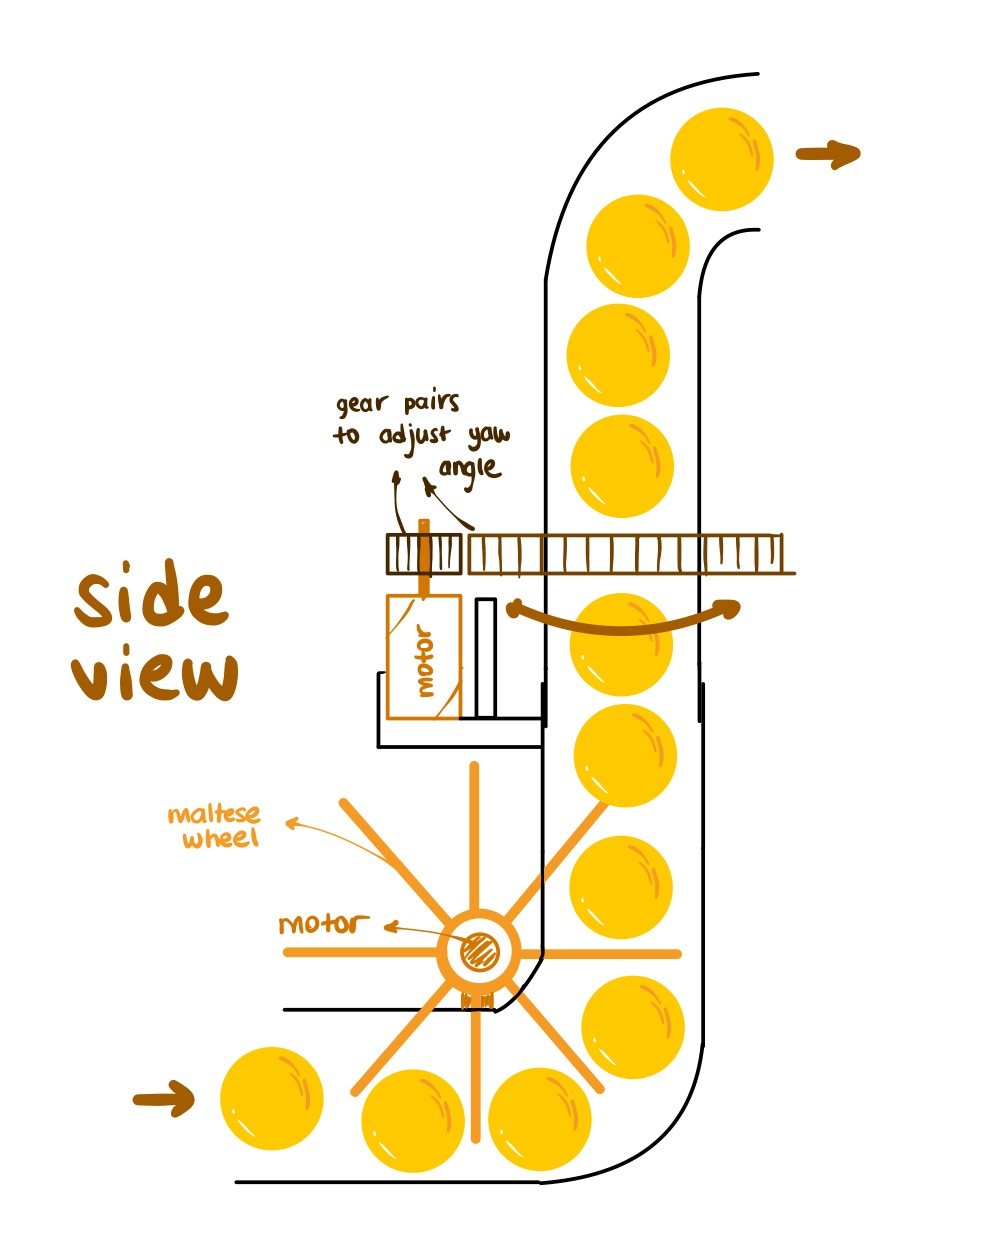
\includegraphics[width=\textwidth]{best_concept/side_feeder.jpeg}
    \captionof{figure}{Feeder side view}
    \vspace{1em}
    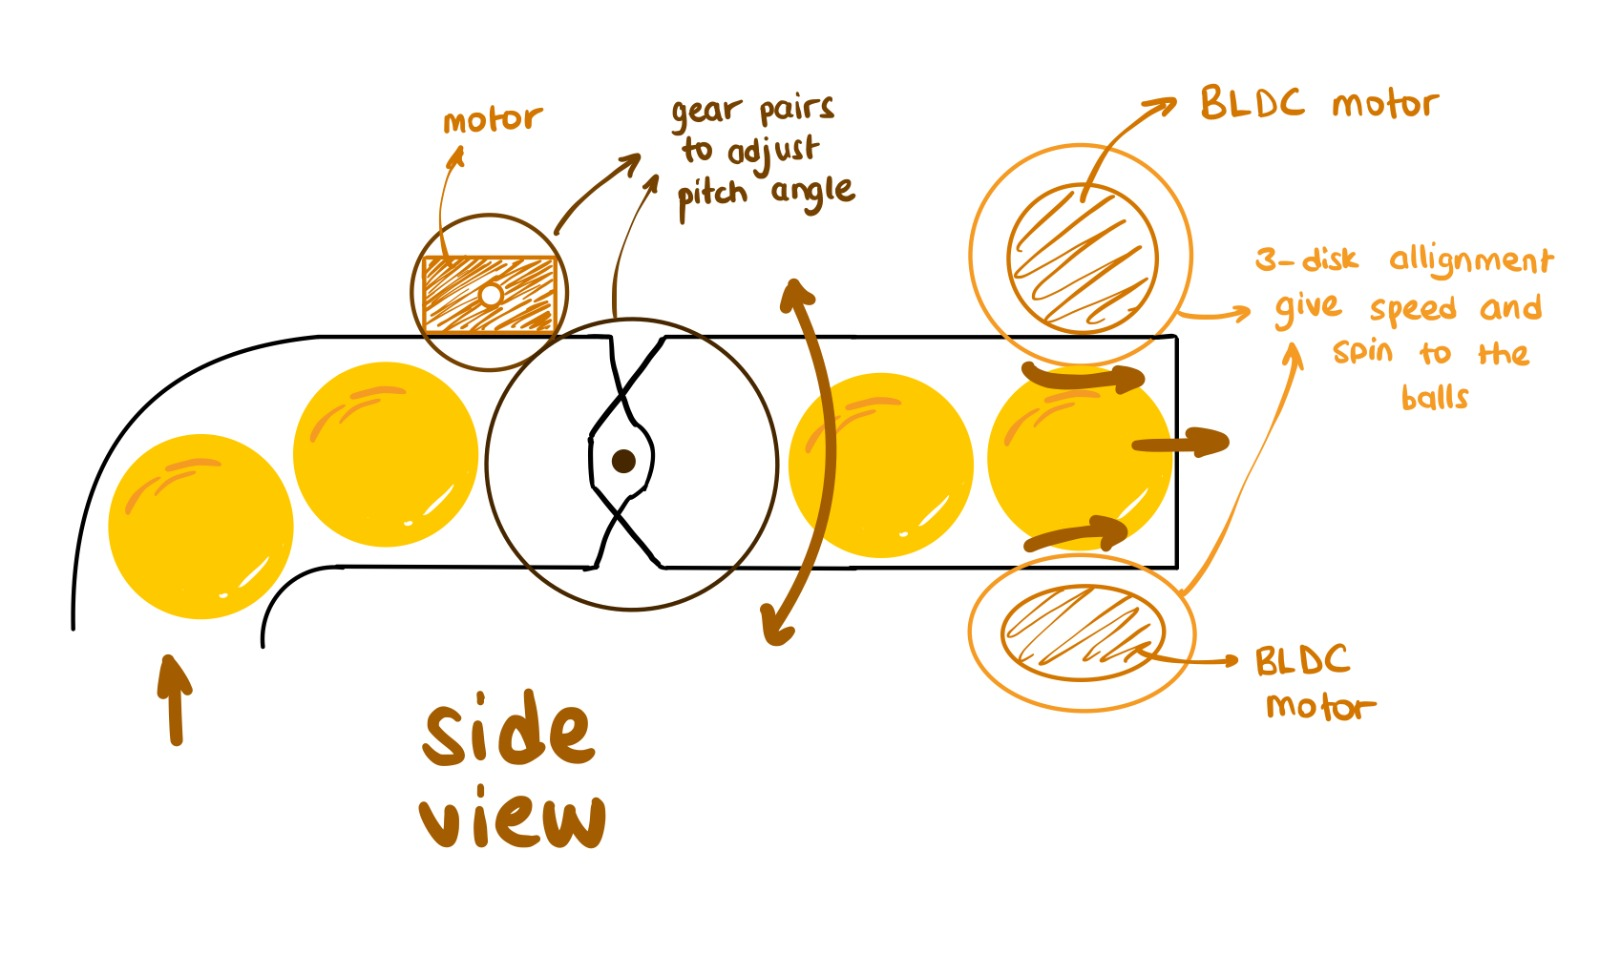
\includegraphics[width=0.9\textwidth]{best_concept/side.jpeg}
    \captionof{figure}{Side view}
    \vspace{1em}
    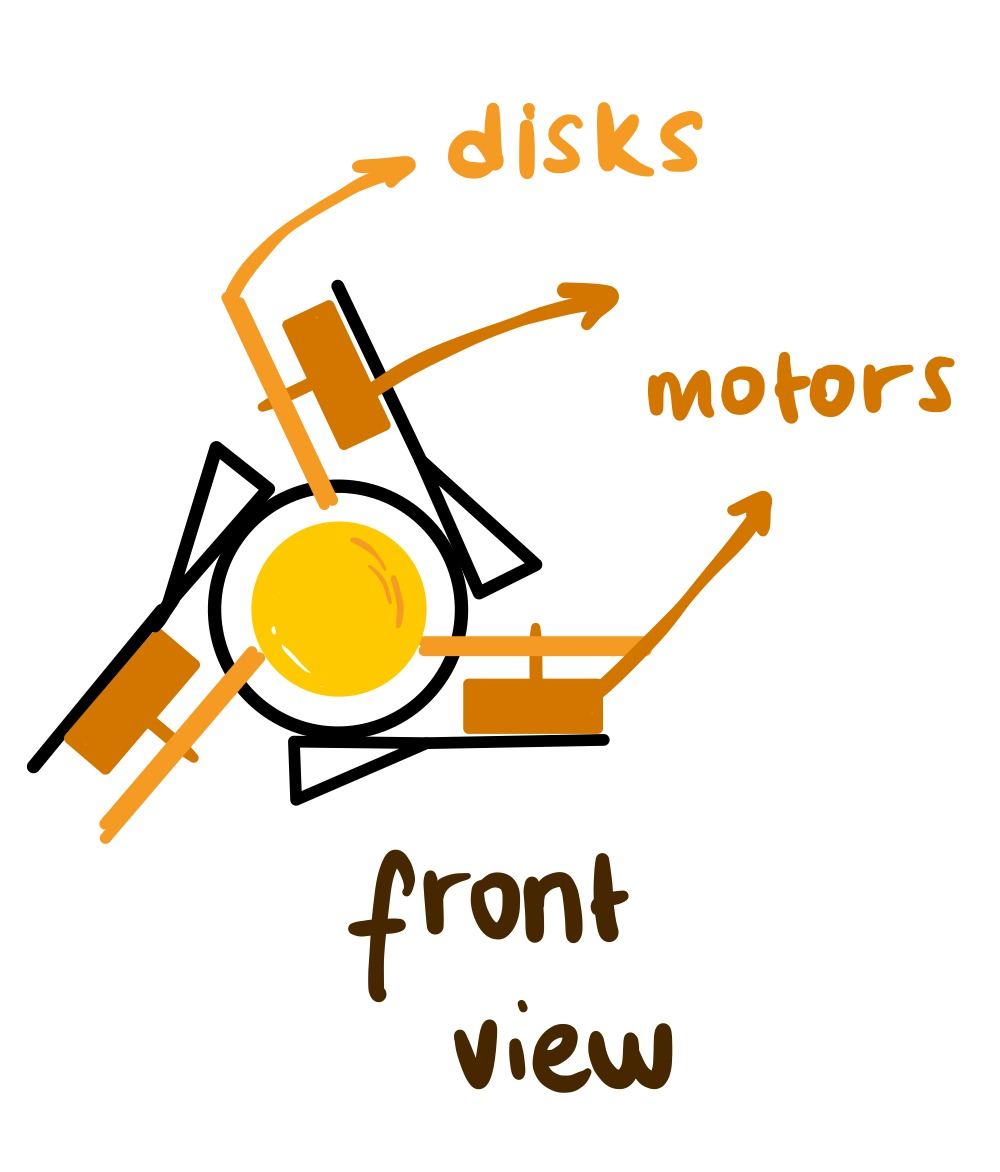
\includegraphics[width=0.5\textwidth]{best_concept/front.jpeg}
    \captionof{figure}{Front View}
\end{minipage}


\begin{figure}[H]
    \centering
    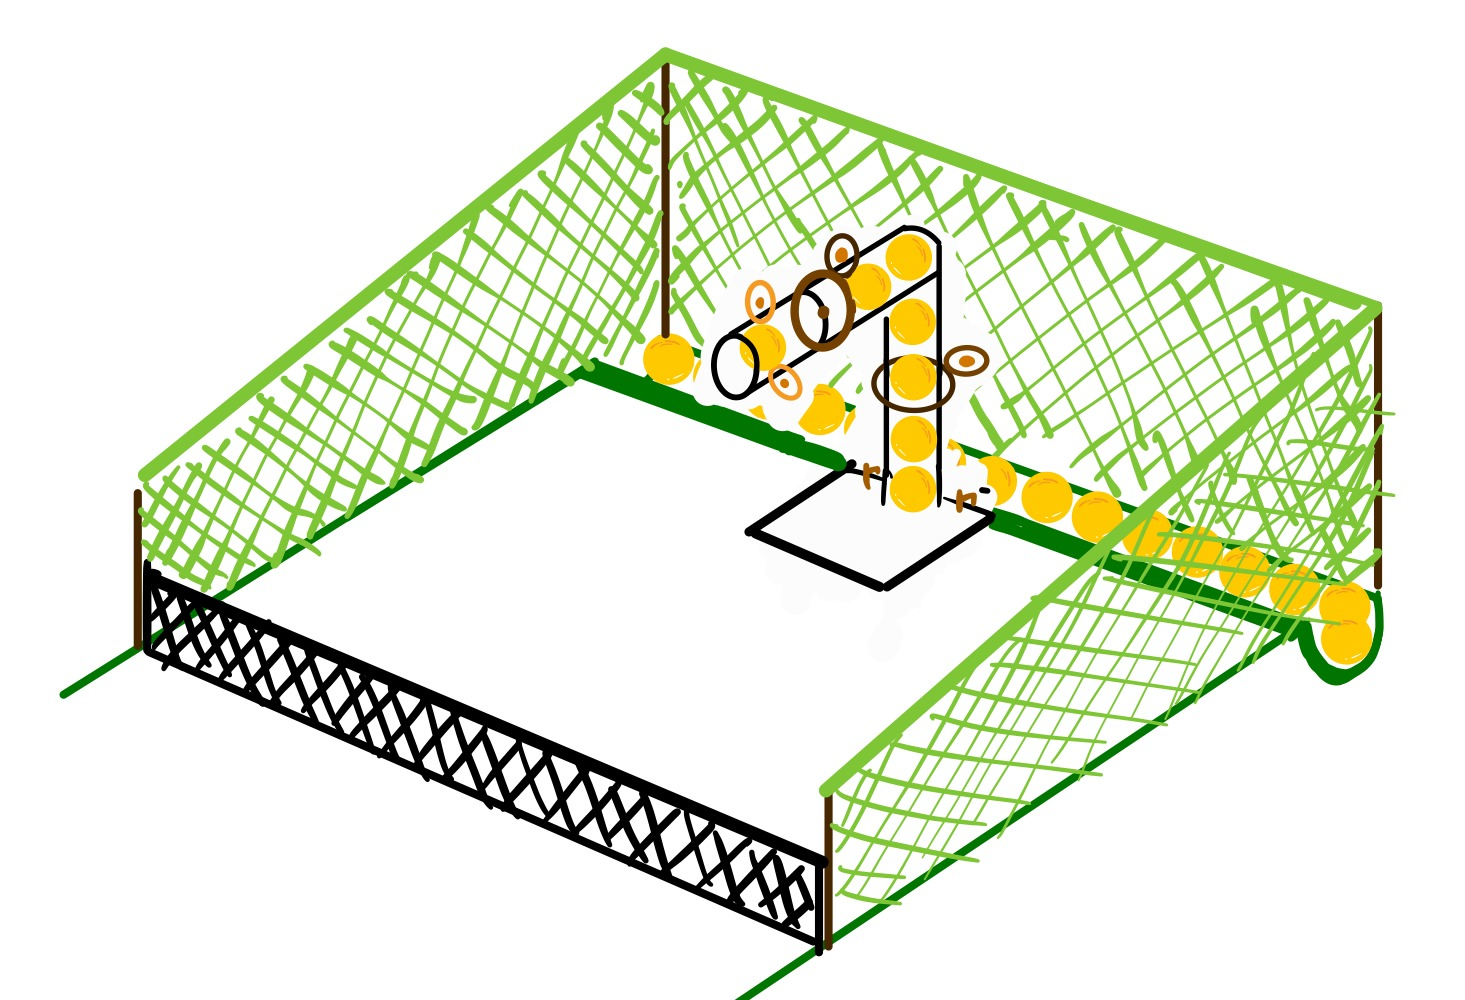
\includegraphics[width=0.5\textwidth]{best_concept/whole.jpeg}
    \caption{Orthogonal view}
    \label{fig:whole_best}
\end{figure}


\section{Summary and Conclusion}

In this report, development of the conceptual design of the project of a Table Tennis Ball Pitcher Machine is presented. The sub-function concepts listed in the Morphological Chart created in the previous steps of the project are evaluated according to the relevant design criteria, and decision matrices are created for each to decide on the most viable options. Then, from these sub-functions, eight different overall concepts are developed by using the combination of different ideas together and observing how the different mechanisms complement each other so as to create the best functional alternatives for the task. What is next is to then evaluate these eight concepts with the overall design criteria to choose the best concept among them. This approach ensures that the concept chosen to proceed with the project brings the most efficient and effective solutions to project requirements, and is the best selection compared to the other alternatives brought up.

\section{Appendix}
\subsection{Function Concepts}

\begin{figure}[H]
\centering
\begin{subfigure}{.3\textwidth}
  \centering
  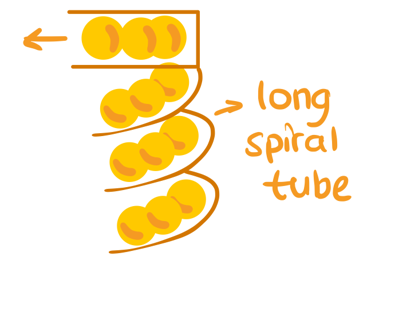
\includegraphics[width=.3\linewidth]{Function photos/Tunnel.png}
  \caption{Tunnel Mechanism}
  \label{fig:tunnel_mechanism}
\end{subfigure}%
\begin{subfigure}{.3\textwidth}
  \centering
  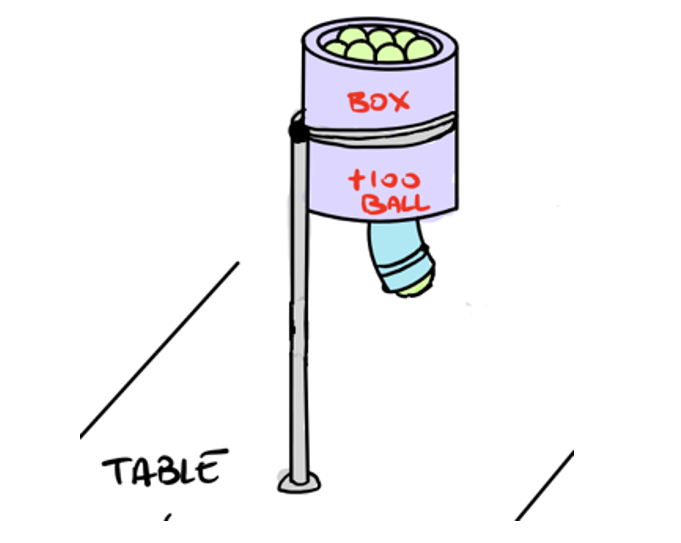
\includegraphics[width=.3\linewidth]{Function photos/box.png}
  \caption{Box}
  \label{fig:box}
\end{subfigure}
\begin{subfigure}{.3\textwidth}
  \centering
  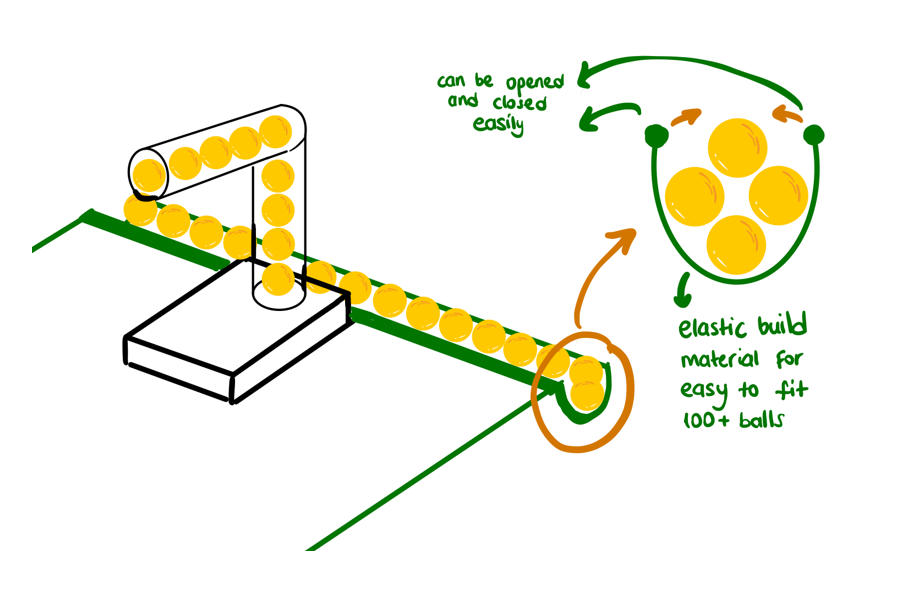
\includegraphics[width=.3\linewidth]{Function photos/groove.png}
  \caption{Groove Mechanism}
  \label{fig:groove_mechanism}
\end{subfigure}%
\caption{Storing Mechanisms}
\label{fig:storing_mechanism}
\end{figure}

\begin{figure}[H]
\centering
\begin{subfigure}{.5\textwidth}
  \centering
  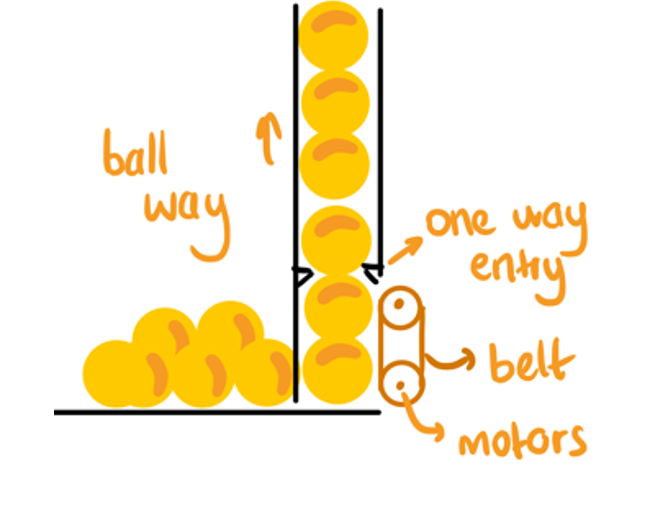
\includegraphics[width=.4\linewidth]{Function photos/Belt.png}
  \caption{Belt}
  \label{fig:belt}
\end{subfigure}%
\begin{subfigure}{.5\textwidth}
  \centering
  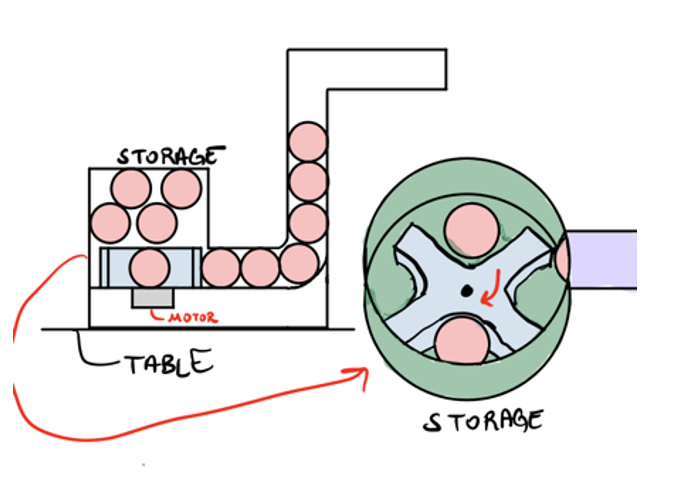
\includegraphics[width=.4\linewidth]{Function photos/maltese 1.png}
  \caption{Maltese wheel}
  \label{fig:maltese}
\end{subfigure}
\begin{subfigure}{.5\textwidth}
  \centering
  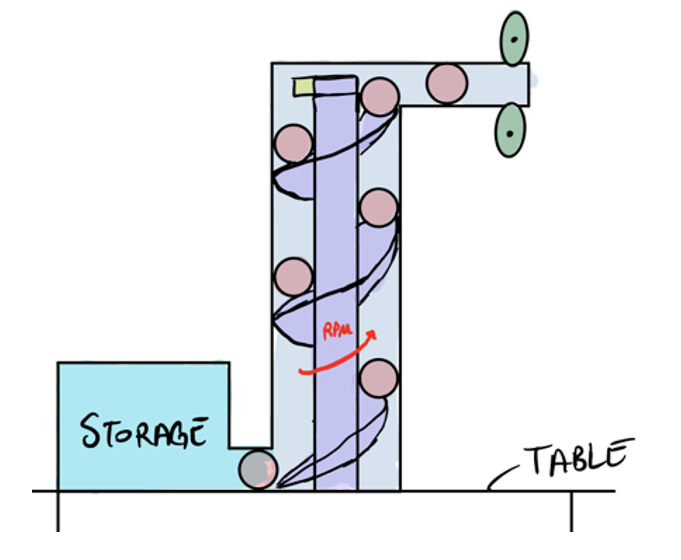
\includegraphics[width=.4\linewidth]{Function photos/spiral.png}
  \caption{Spiral mechanism}
  \label{fig:spiral}
\end{subfigure}%
\begin{subfigure}{.5\textwidth}
  \centering
  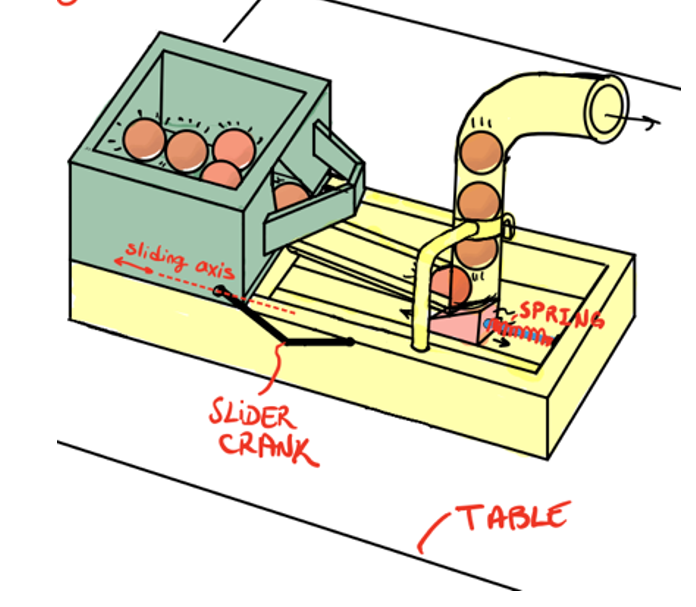
\includegraphics[width=.4\linewidth]{Function photos/Translating Box.png}
  \caption{Translating Box}
  \label{fig:translating_box}
\end{subfigure}%
\caption{Transferring the balls from storage }
\label{fig:transferring_storage}
\end{figure}

\begin{figure}[H]
\centering
\begin{subfigure}{.5\textwidth}
  \centering
  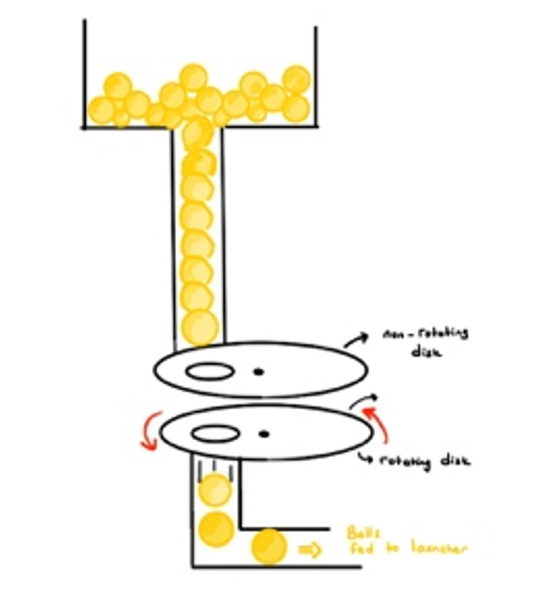
\includegraphics[width=.4\linewidth]{Function photos/rotating hole.png}
  \caption{Rotating Hole}
  \label{fig:rotating_hole}
\end{subfigure}%
\begin{subfigure}{.5\textwidth}
  \centering
  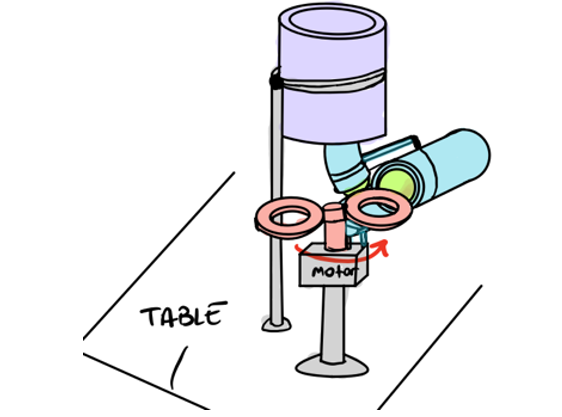
\includegraphics[width=.4\linewidth]{Function photos/Rotating Pusher.png}
  \caption{Rotating Pusher}
  \label{fig:rotating_pusher}
\end{subfigure}
\begin{subfigure}{.5\textwidth}
  \centering
  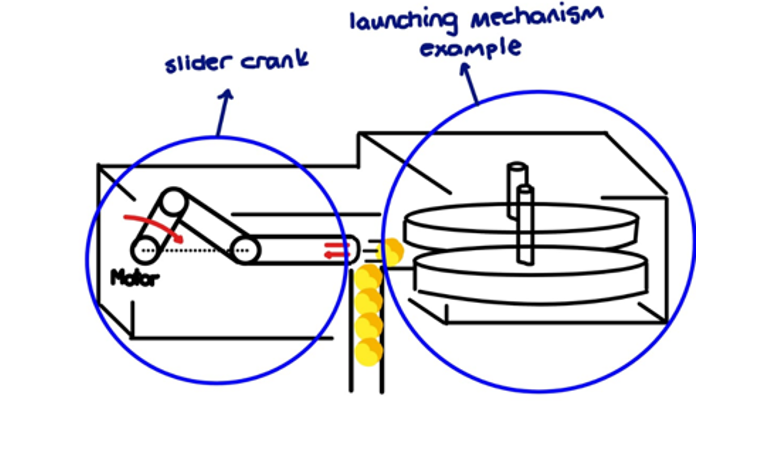
\includegraphics[width=.4\linewidth]{Function photos/Slider Crank.png}
  \caption{Slider Crank}
  \label{fig:slider_crank}
\end{subfigure}%
\begin{subfigure}{.5\textwidth}
  \centering
  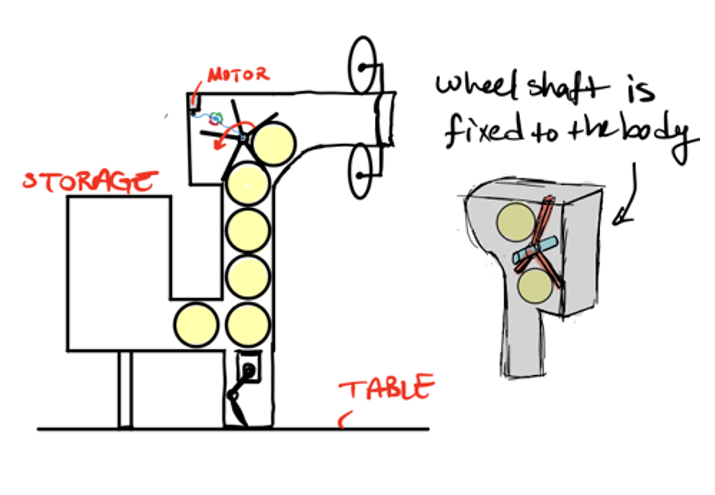
\includegraphics[width=.4\linewidth]{Function photos/maltese 2.png}
  \caption{Maltese wheel}
  \label{fig:maltese_wheel}
\end{subfigure}%

\begin{subfigure}{.5\textwidth}
  \centering
  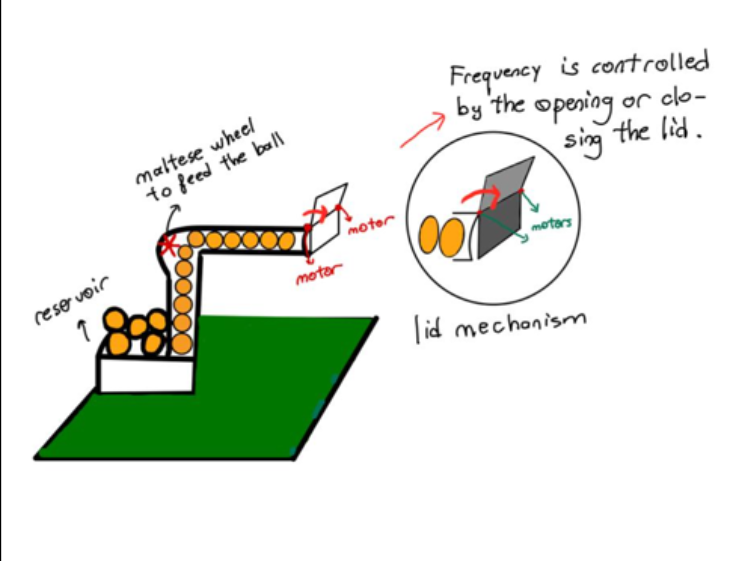
\includegraphics[width=.4\linewidth]{lid.png}
  \caption{Lid Mechanism}
  \label{fig:lid_mechanism}
\end{subfigure}%
\begin{subfigure}{.5\textwidth}
  \centering
  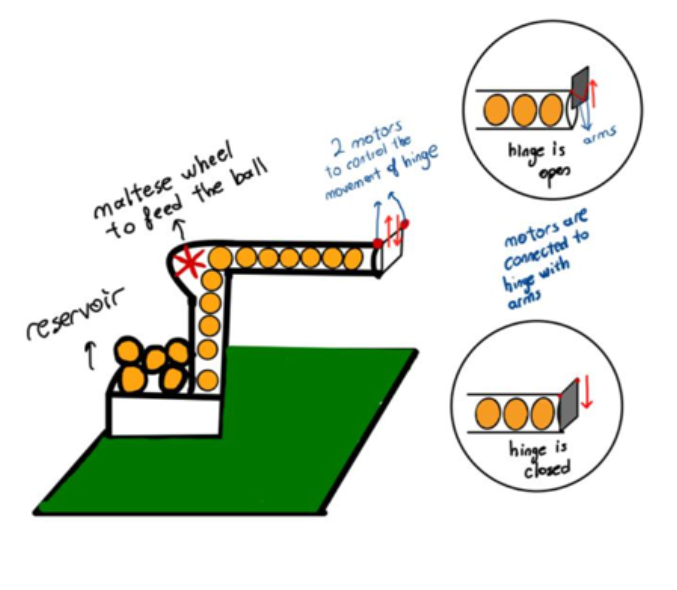
\includegraphics[width=.4\linewidth]{hinge.png}
  \caption{Hinge Mechanism}
  \label{fig:hinge_mechanism}
\end{subfigure}%


\caption{Giving the balls desired frequency}
\label{fig:giving_frequency}
\end{figure}

\begin{figure}[H]
\centering
\begin{minipage}{.5\textwidth}
  \centering
  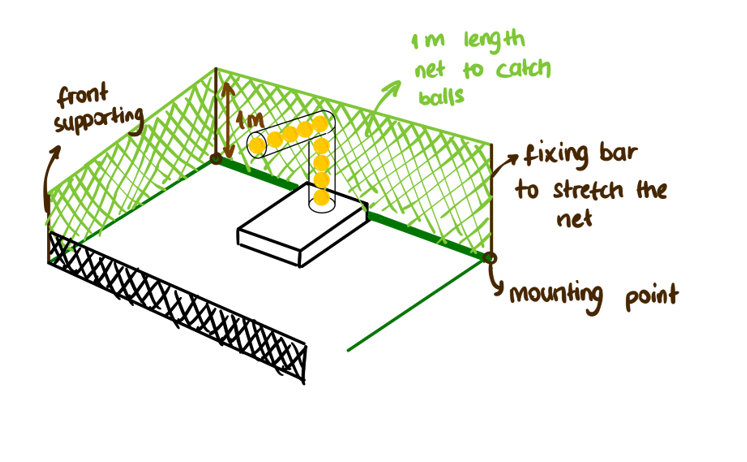
\includegraphics[width=.4\linewidth]{Function photos/net.png}
  \captionof{figure}{Net}
  \label{fig:net}
\end{minipage}%
\begin{minipage}{.5\textwidth}
  \centering
  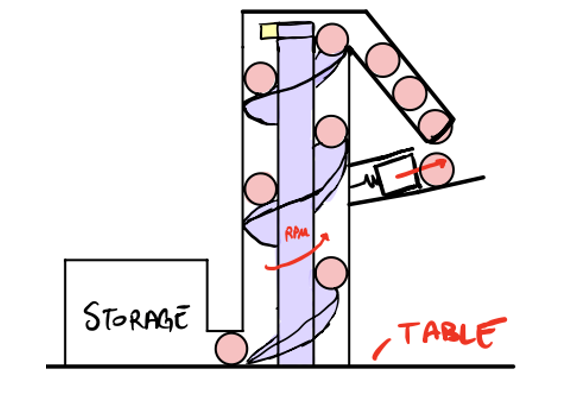
\includegraphics[width=.4\linewidth]{Function photos/gravity.png}
  \captionof{figure}{Gravity Mechanism}
  \label{fig:gravity}
\end{minipage}
\end{figure}



\begin{figure}[H]
\centering
\begin{subfigure}{.5\textwidth}
  \centering
  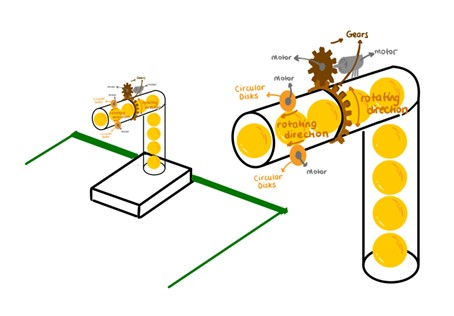
\includegraphics[width=.4\linewidth]{2 wheels and spinning head.jpg}
  \caption{2 wheels and spinning head}
  \label{fig:2wheel}
\end{subfigure}%
\begin{subfigure}{.5\textwidth}
  \centering
  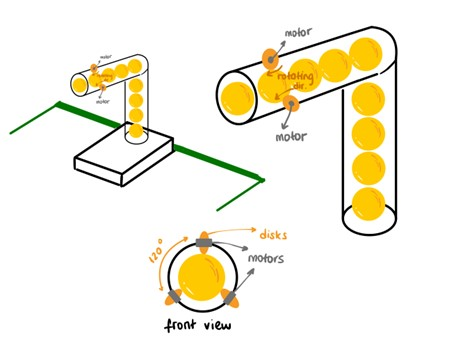
\includegraphics[width=.4\linewidth]{3 wheels.jpg}
  \caption{3 wheels}
  \label{fig:3wheel}
\end{subfigure}
\begin{subfigure}{.5\textwidth}
  \centering
  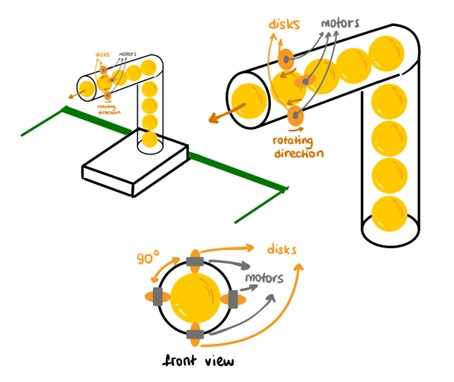
\includegraphics[width=.4\linewidth]{4 wheels.jpg}
  \caption{4 wheels}
  \label{fig:4wheel}
\end{subfigure}%
\begin{subfigure}{.5\textwidth}
  \centering
  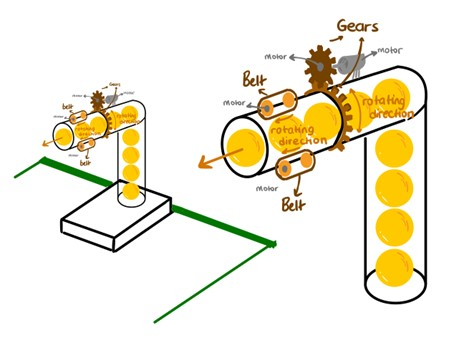
\includegraphics[width=.4\linewidth]{2 tension belt with spinning head.jpg}
  \caption{2 tension belt with spinning head}
  \label{fig:2tension}
\end{subfigure}%

\begin{subfigure}{.5\textwidth}
  \centering
  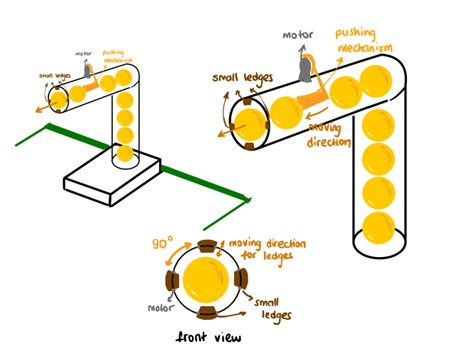
\includegraphics[width=.4\linewidth]{Small legdes with friction pad.jpg}
  \caption{Small ledges with friction pad}
  \label{fig:ledges}
\end{subfigure}%
\begin{subfigure}{.5\textwidth}
  \centering
  
  \label{fig:spins}
\end{subfigure}%


\caption{Giving spin and speed to the balls  }
\label{fig:test}
\end{figure}

\begin{figure}[H]
\centering
\begin{subfigure}{.5\textwidth}
  \centering
  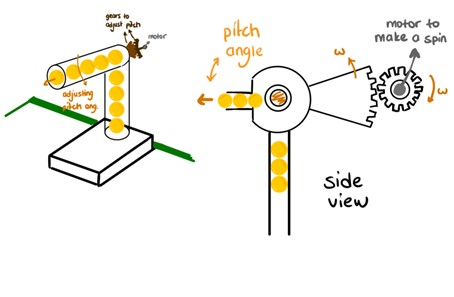
\includegraphics[width=.4\linewidth]{gearpitch.jpg}
  \caption{Gear}
  \label{fig:gear}
\end{subfigure}%
\begin{subfigure}{.5\textwidth}
  \centering
  \includegraphics[width=.4\linewidth]{wormpitch.jpg}
  \caption{Single worm gear}
  \label{fig:worm}
\end{subfigure}
\begin{subfigure}{.5\textwidth}
  \centering
  \includegraphics[width=.4\linewidth]{bevelpitch.jpg}
  \caption{Bevel gear}
  \label{fig:bevel}
\end{subfigure}%
\begin{subfigure}{.5\textwidth}
  \centering
  \includegraphics[width=.4\linewidth]{fourbarpitch.jpg}
  \caption{Four bar mechanism}
  \label{fig:fourbar}
\end{subfigure}%

\begin{subfigure}{.5\textwidth}
  \centering
  \includegraphics[width=.4\linewidth]{ropecontrol.jpg}
  \caption{Rope-controlled head pulley}
  \label{fig:rope}
\end{subfigure}%

\caption{Giving pitch angle to the launching mechanism  }
\label{fig:pitch}
\end{figure}


\begin{figure}[H]
\centering
\begin{subfigure}{.5\textwidth}
  \centering
  \includegraphics[width=.4\linewidth]{gear1yaw.jpg}
  \caption{Gear 1}
  \label{fig:gear1}
\end{subfigure}%
\begin{subfigure}{.5\textwidth}
  \centering
  \includegraphics[width=.4\linewidth]{gear2yaw.jpg}
  \caption{Gear 2}
  \label{fig:gear2}
\end{subfigure}
\begin{subfigure}{.5\textwidth}
  \centering
  \includegraphics[width=.4\linewidth]{wormyaw.jpg}
  \caption{Worm gear}
  \label{fig:worm_yaw}
\end{subfigure}%
\begin{subfigure}{.5\textwidth}
  \centering
  \includegraphics[width=.4\linewidth]{bevelyaw.jpg}
  \caption{Bevel gear}
  \label{fig:bevel_yaw}
\end{subfigure}%

\begin{subfigure}{.5\textwidth}
  \centering
  \includegraphics[width=.4\linewidth]{fourbaryaw.jpg}
  \caption{Four bar mechanism}
  \label{fig:fourbar_yaw}
\end{subfigure}%

\caption{Giving yaw angle to the launching mechanism  }
\label{fig:yaw}
\end{figure}

\begin{figure}[H]
\centering
\begin{subfigure}{.3\textwidth}
  \centering
  \includegraphics[width=.3\linewidth]{integratedcontroller.jpg}
  \caption{Integrated controller}
  \label{fig:integrated}
\end{subfigure}%
\begin{subfigure}{.3\textwidth}
  \centering
  \includegraphics[width=.3\linewidth]{wiredremote.jpg}
  \caption{Wired remote controller}
  \label{fig:wired}
\end{subfigure}

\caption{Accepting spin and frequency information from the user}
\label{fig:accept_spin_freq}
\end{figure}

\begin{figure}[H]
\centering
\begin{subfigure}{.3\textwidth}
  \centering
  \includegraphics[width=.3\linewidth]{potentiometer.jpg}
  \caption{Potentiometer with buttons}
  \label{fig:pot}
\end{subfigure}%
\begin{subfigure}{.3\textwidth}
  \centering
  \includegraphics[width=.3\linewidth]{encoder.jpg}
  \caption{Encoder with buttons}
  \label{fig:encoder}
\end{subfigure}

\caption{Accepting speed information from the user}
\label{fig:accept_speed}
\end{figure}

\begin{figure}[H]
\centering

  \includegraphics[width=.2\linewidth]{clamps.jpg}
  \caption{Clamps}
  \label{fig:clamp}

\end{figure}

\subsection{Morphological Chart \label{app:morpho}}

\begin{center}
    \includegraphics[width=1.4\textwidth, page=1, angle=90]{morphological.pdf}
\end{center}


\begin{center}
    \includegraphics[width=1.4\textwidth, page=2, angle=90]{morphological.pdf} % Adjust width as needed
\end{center}

\begin{center}
    \includegraphics[width=1.4\textwidth, page=3, angle=90]{morphological.pdf} % Adjust width as needed
\end{center}

\begin{center}
    \includegraphics[width=1.4\textwidth, page=4, angle=90]{morphological.pdf} % Adjust width as needed
\end{center}

\begin{center}
    \includegraphics[width=1.4\textwidth, page=5, angle=90]{morphological.pdf} % Adjust width as needed
\end{center}

% Prevent floats from passing this point
\FloatBarrier


% % References section
% \bibliographystyle{IEEEtran} % or any style you prefer
% \bibliography{bibliography}

\end{document}
